% August 2017 (TOC contents linked in blue in pdf file)
%This template was prepared by Dorothea F. Brosius of the
%Institute for Electronics and Applied Physics, University of Maryland, College Park, MD
%The template was last updated in August 2017
%Thesis Main Page used with thesis.sty based on the
%University of Maryland Electronic Thesis and Dissertation (ETD) Style Guide (2016)

%The YourInformation file was created by Freja Nordsiek, 2014.
%Code for linking the TOC titles to the texyt in the pdf file was created by Freja Nordsiek, 2014.

% Select the version that fits how you are making this LaTeX document (its driver).
% The first two are the most likely ones to be needed.

\newcommand{\mydriver}{pdflatex} %Making a PDF directly using pdflatex.

\documentclass[12pt,\mydriver]{style/umd-thesis/thesis}  %12pt is larger than 11pt

\usepackage[normalem]{ulem}
\usepackage[utf8]{inputenc} % allow utf-8 input
\usepackage[T1]{fontenc}    % use 8-bit T1 fonts
\usepackage{epstopdf}
\usepackage{wrapfig}
\usepackage{nicefrac}
\usepackage{amsfonts}
\usepackage{url}
%\usepackage{subeqn}
\usepackage{dsfont}
\usepackage{caption}
\usepackage{subcaption}
\usepackage{comment}
\usepackage{graphicx}
\usepackage{natbib}
\usepackage{bibentry}
\usepackage{xspace}
\usepackage{bm,bbm}
\usepackage{algorithm,algorithmicx,algpseudocode}
\usepackage{amsmath,amssymb}
\usepackage{latexsym}
\usepackage{hhline}
\usepackage{mdwlist}
\usepackage{url}
\usepackage{color,xcolor,colortbl}
\usepackage{tikzsymbols}
\usepackage{tikz}
\usepackage{booktabs}
\usepackage{csquotes}
\usepackage{amsfonts}
%\usepackage{marvosym}
\usepackage{tabularx}
\usepackage{pifont}% http://ctan.org/pkg/pifont
\usepackage{soul}
\usepackage{epigraph}
\usepackage{enumitem}
\usepackage{mdwlist}

\setlength\epigraphwidth{.8\textwidth}
\DeclareMathOperator*{\argmax}{arg\,max}
\usetikzlibrary{tikzmark}
\usepackage{colortbl}

\usepackage{style/umd-thesis/titlesec}
   \titleformat{\chapter}
      {\normalfont\large}{Chapter \thechapter:}{1em}{}
\usepackage{style/umd-thesis/cite}
\usepackage{style/umd-thesis/lscape}
\usepackage{style/umd-thesis/indentfirst}
\usepackage{style/umd-thesis/latexsym}
\usepackage{style/umd-thesis/multirow}
%\usepackage{style/umd-thesis/tabls}
\usepackage{style/umd-thesis/longtable}
\usepackage{style/umd-thesis/supertabular}
\usepackage{style/umd-thesis/slashbox}
\usepackage[colorlinks=true,urlcolor=black,linkcolor=blue,citecolor=blue]{hyperref}
\usepackage{natbib}
\usepackage{bibentry}

\makeatletter
\patchcmd{\SOUL@ulunderline}{\dimen@}{\SOUL@dimen}{}{}
\patchcmd{\SOUL@ulunderline}{\dimen@}{\SOUL@dimen}{}{}
\patchcmd{\SOUL@ulunderline}{\dimen@}{\SOUL@dimen}{}{}
\newdimen\SOUL@dimen
\makeatother


\newif\ifcomment
\commentfalse

% colors
\definecolor{mycolor}{HTML}{9EE6FF}

% Shortcuts
\newcommand{\dan}[0]{\abr{dan}}
\newcommand{\lstm}[0]{\abr{lstm}}
\newcommand{\gru}[0]{\abr{gru}}
\newcommand{\qa}[0]{\abr{qa}}
\newcommand{\mt}[0]{\abr{mt}}
\newcommand{\qb}[0]{\abr{qb}}
\newcommand{\ngram}[0]{$n$-gram}
\newcommand{\nlp}[0]{\abr{nlp}}
\newcommand{\iaa}[0]{\abr{iaa}}
\newcommand{\nq}[0]{\abr{nq}}
\newcommand{\squad}{\textsc{sq}{\small u}\textsc{ad}}
\newcommand{\quac}{\textsc{q}{\small u}\textsc{ac}}
\newcommand{\coqa}{\textsc{c}{\small o}\textsc{qa}}
\newcommand{\conll}{\textsc{c}{\small o}\textsc{nll}}
\newcommand{\cove}{\textsc{c}{\small o}\textsc{v}{\small e}}
\newcommand{\elmo}{\textsc{elm}{\small o}}
\newcommand{\fone}{$F_1$}
\newcommand{\tfidf}{\abr{tf-idf}}
\newcommand{\rnn}{\abr{rnn}}
\newcommand{\qanta}{\abr{qanta}}
\newcommand{\trec}{\abr{trec}}
\newcommand{\bleu}{\abr{bleu}}
\newcommand{\entity}[1] {\uline{#1}}

%Diplomacy
\newcommand{\autofig}[1]{denis_proposal/sections/diplomacy/auto_fig/#1}
\newcommand{\figfile}[1]{denis_proposal/figures/#1}
%\newcommand{\figfile}[1]{denis_proposal/sections/diplomacy/figures/#1}
\newcommand{\alie}{\textsc{actual lie}}
\newcommand{\slie}{\textsc{suspected lie}}
\newcommand{\player}[1]{\underline{#1}}
\newcommand{\totalnumber}{17,289}
\newcommand{\wordlist}{Harbingers}


%MultiDoGo
\definecolor{LightCyan}{rgb}{0.88,1,1}
\definecolor{Gray}{gray}{0.95}
\newcolumntype{a}{>{\columncolor{Gray}}c}
\newcommand\BibTeX{B\textsc{ib}\TeX}
\newcommand{\multiwoz}{\texttt{MultiWOZ}\xspace}
\newcommand{\multidogo}{\texttt{MultiDoGO}\xspace}

%InterSpeech
\newcommand{\asr}{\textsc{asr}}
\newcommand{\unk}{<\textit{unk}>}

\newcommand{\name} {\abr{canard}}


%ContraCAT
\newcommand{\coref}{\textsc{cr}}
\newcommand{\nmt}{\textsc{nmt}}
\newcommand{\cat}{\textit{cat}}
\newcommand{\stepone}{Markable Detection}
\newcommand{\steptwo}{Coreference Resolution}
\newcommand{\stepthree}{Language Translation}
\newcommand{\contracat}{Contra\textsc{cat}}

% Functions
\newcommand{\norm}[1]{| #1 |}
\newcommand{\abs}[1]{\lvert #1 \rvert}
\newcommand{\feat}[1]{{\small \texttt{#1}}}
\newcommand{\act}[1]{{\small \texttt{#1}}}
\newcommand{\gem}[1]{\mbox{\textsc{gem}}}
\newcommand{\abr}[1]{\textsc{#1}}
\newcommand{\camelabr}[2]{{\small #1}{\textsc{#2}}}
\newcommand{\abrcamel}[2]{{\textsc #1}{\small{#2}}}
\newcommand{\grammar}[1]{{\color{red} #1}}
\newcommand{\explain}[2]{\underbrace{#2}_{\mbox{\footnotesize{#1}}}}
\newcommand{\dir}[1]{\mbox{Dir}(#1)}
\newcommand{\bet}[1]{\mbox{Beta}(#1)}
\newcommand{\py}[1]{\mbox{\textsc{py}}(#1)}
\newcommand{\td}[2]{\mbox{\textsc{TreeDist}}_{#1} \left( #2 \right)}
\newcommand{\yield}[1]{\mbox{\textsc{Yield}} \left( #1 \right)}
\newcommand{\mult}[1]{\mbox{Mult}( #1)}
\newcommand{\wn}{\textsc{WordNet}}
\newcommand{\twentynews}{\textsc{20news}}
\newcommand{\g}{\, | \,}
\newcommand{\Gam}[1]{\Gamma \left( \textstyle #1 \right)}
\newcommand{\LG}[1]{\log \Gamma \left( \textstyle #1 \right)}
\newcommand{\Pois}[1]{\mbox{Poisson}(#1)}
\newcommand{\pcfg}[3]{#1_{#2 \rightarrow #3}}
\newcommand{\grule}[2]{#1 \rightarrow #2}
\newcommand{\kl}[2]{D_{\mbox{\textsc{KL}}} \left( #1 \,||\, #2 \right)}
\newcommand{\iemph}[1]{\textit{#1}}

\newcommand{\digambig}[1]{\Psi \left( #1 \right) }
\newcommand{\digam}[1]{\Psi \left( \textstyle #1 \right) }
\newcommand{\ddigam}[1]{\Psi' \left( \textstyle #1 \right) }
\newcommand{\tbsp}{\rule{0pt}{18pt}} %used to get a vertical distance after \hline
\renewcommand{\baselinestretch}{2}

\setlength{\textwidth}{5.9in}
\setlength{\textheight}{9in}
\setlength{\topmargin}{-.50in}
%\setlength{\topmargin}{0in}    %use this setting if the printer makes the the top margin 1/2 inch instead of 1 inch
\setlength{\oddsidemargin}{.55in}
\setlength{\parindent}{.4in}
\pagestyle{empty}

% Comments
\newcommand{\hidetext}[1]{}
\newcommand{\ignore}[1]{}

\newcommand{\todo}[1]{\textcolor{red}{{\bf TODO: #1}}}

\ifcomment
  \newcommand{\pinaforecomment}[3]{\colorbox{#1}{\parbox{.8\linewidth}{#2: #3}}}
\else
  \newcommand{\pinaforecomment}[3]{}
\fi
\newcommand{\jbgcomment}[1]{\pinaforecomment{red}{JBG}{#1}}
\newcommand{\dpcomment}[1]{\pinaforecomment{blue}{Denis}{#1}}

\newcommand*{\TakeFourierOrnament}[1]{{%
      \fontencoding{U}\fontfamily{futs}\selectfont\char#1}}
\newcommand*{\danger}{\TakeFourierOrnament{66}}
\newcommand\cmark {\textcolor{green}{\ding{52}~}}
\newcommand\cmarktight {\textcolor{green}{\ding{52}}}
\newcommand\xmark {\textcolor{red}{\ding{55}~}}
\newcommand\xmarktight {\textcolor{red}{\ding{55}}}
\newcommand\dmark {\textcolor{yellow}{\danger}}
\newcommand{\challenge}{adversarially authored}

\graphicspath{{denis_proposal/figures/}{denis_proposal/commit_auto_fig/}{denis_proposal/auto_fig/}}


\begin{document}
\nobibliography*
\pagestyle{empty}
%Abstract Page

\hbox{\ }

\renewcommand{\baselinestretch}{1}
\small \normalsize

\begin{center}
    \large{{ABSTRACT}}
    
    \vspace{3em}
    
\end{center}
\hspace{-.15in}
\begin{tabular}{ll}
    Title of proposal: & {\large  Gathering Language Data Using Experts}     \\
    \                                                                      \\
                       & {\large  Denis Peskov, 2020}                   \\
    %&                           {\large Doctor of Philosophy, 2004} \\
    \                                                                      \\
    Dissertation directed by:
                       & {\large  Professor Jordan Boyd-Graber}            \\
                       & {\large  Department of Computer Science}          \\
                       & {\large  College of Information Studies}          \\
                       & {\large  Language Science Center}                 \\
                       & {\large  Institute for Advanced Computer Studies} \\
\end{tabular}

\vspace{3em}

\renewcommand{\baselinestretch}{2}
\large \normalsize


Natural Language Processing needs substantial data to make robust predictions. 
%
Automatic methods, unspecialized crowds, and domain experts can be used to collect this prerequisite data.
%
We curate large-scale conversational and question answering \abr{nlp} datasets using these various methods. 


A low-cost, high-output approach to data creation is \textit{automation}.  
%
We explore this approach by creating and analyzing a large-scale audio question answering dataset through text-to-speech technology.  
%
%However, in Quizbowl questions are read at an unusually fast pace and involve highly technical and multi-cultural words causing a disparity between automation and reality.  
%
We conclude that the cost-savings and scalability of automation come at the cost of data quality and naturalness.  

Human input can provide this degree of naturalness, but is limited in scale. 
%
Hence, large-scale data collection is frequently done through \textit{crowd-sourcing}.
%
A question-rewriting task, in which a long information-gathering conversation is used as source material for many stand-alone questions, shows the limitation of using this methodology for \textit{generating} data.
%; however, these have limitations as noted in two question answering projects: question-rewriting and audio question answering.     
%
%Generating data through crowd-sourcing poses a serious quality control challenge, since 
Standard inter-annotator agreement metrics, while useful for \textit{annotation}, cannot easily evaluate \textit{generated} data, causing a serious quality control issue.  
%
This problem is observed while formalizing a question-rewriting task; certain users provide low-quality rewrites---removing words from the question, copy and pasting the answer into the question---if left unsupervised.  
%
We automatically prevent unsatisfactory submissions through an interface, but the quality control process still requires manually reviewing over 5,000 questions.  

Certain users provide more reliable annotations and generations than others, which can be used to improve the quality control process.  
%
%We mitigate the quality control issues identified in crowd-sourcing and automation through exploring
\textit{Hybrid} solutions pair potentially unreliable and unverified users in the crowd with experts.  
%
As an example, Amazon customer service agents are used for curation and annotation of goal-oriented 81,000 conversations across six domains.  
%
By grounding the conversation with a reliable conversationalist---the Amazon agent---we create untemplated conversations and reliably identify low-quality conversations.    
%
The sentences generated from crowd workers are less natural and diverse than those from experts.   

Therefore, we posit that exclusively using domain \textit{experts} for data generation can create novel and reliable \abr{nlp} datasets. 
%
In a study on the game of Diplomacy, which investigates the language of trust and deception, Diplomacy community members generate a corpus of 17,000 messages that are self-annotated while playing a game. 
%
The language is varied in length, tone, vocabulary, punctuation, and even emojis.
%
Additionally, we create a real-time self-annotation system that annotates deception in a manner not possible through  crowd-sourced or automatic methods.  
%Annotation based on a user's perception can change ex-post-facto; a duped user may in retrospect conclude that they had expected a lie when reality suggests otherwise.   
 %
%Hence, real-time annotation by the original user is integral to this task.  
 %
We propose future work that leverages experts to create a new machine translation task: \textit{cultural adaptation}.  
 %
%Identifying relevant communities for a specific NLP task, and providing a service to them can set new standards for NLP corpora.  
 
 %(must be first, required, non-numbered)
%Titlepage

\thispagestyle{empty}
\hbox{\ }
\vspace{1in}
\renewcommand{\baselinestretch}{1}
\small\normalsize
\begin{center}

    \large{{Gathering Natural Language Processing Data Using Experts}}   \\
    \ \\
    \ \\
    \large{by} \\
    \ \\
    \large{Denis Peskov}%Your full name as it appears in University records.
    \ \\
    \ \\
    \ \\
    \ \\
    \normalsize
    Dissertation proposal submitted to the Faculty of the Graduate School of the \\
    University of Maryland, College Park in partial fulfillment \\
    of the requirements for the degree of \\
    Doctor of Philosophy \\
    2020
\end{center}

\vspace{7.5em}

\noindent Advisory Committee: \\
Professor Jordan Boyd-Graber, Chair \\
Professor Michelle Mazurek \\
Professor Philip Resnik \\
 %(must follow Abstract, required, non-numbered)
%Copyright

\thispagestyle{empty}
\hbox{\ }

\vfill
\renewcommand{\baselinestretch}{1}
\small\normalsize

\vspace{-.65in}

\begin{center}
    \large{\copyright \hbox{ }Copyright by\\
        Denis Peskov  %Type your name as it appears in University records
        \\
        2020}
\end{center}

\vfill
 %(highly recommended, non-numbered)

%Pages from this point start at lower- Roman number ii)
\pagestyle{plain} \pagenumbering{roman} \setcounter{page}{2}
%\addcontentsline{toc}{chapter}{Preface}
%\include{weiwei_proposal/sections/Preface}  %(if present, start at lower-case Roman number ii)
%\addcontentsline{toc}{chapter}{Foreword}
%\include{weiwei_proposal/sections/Foreword} %(if present, lower-case Roman)
%\addcontentsline{toc}{chapter}{Dedication}
%\include{weiwei_proposal/sections/Dedication} %(if present, lower-case Roman)
%\addcontentsline{toc}{chapter}{Acknowledgements}
%\include{weiwei_proposal/sections/Acknowledgements} %(if present, lower-case Roman)

\renewcommand{\baselinestretch}{1}
\small\normalsize
\tableofcontents %(required, lower-case Roman)
\newpage
\listoftables %(if present, lower-case Roman)
\newpage
\listoffigures %(if present, lower-case Roman)
\newpage
% LIST OF ABBREVIATIONS
%\addcontentsline{toc}{chapter}{List of Abbreviations}
%\include{weiwei_proposal/sections/Abbreviations-supertabular}

\newpage
\setlength{\parskip}{0em}
\renewcommand{\baselinestretch}{1} % Line stretch, 1 for proposal, 2 for thesis
\small\normalsize

%Pages from this point start at Arabic numeral 1
\setcounter{page}{1}
\pagenumbering{arabic}
% intro
\chapter{The Case for Upfront Investment in Data}
\label{sec:intro}

Computation can solve tasks across multiple areas of scientific inquiry: natural language processing, computer vision, biology, etc.  
%
Solving tasks for all these domains---translating a sentence between languages, distinguishing a cat and a dog, classifying a mutation---has two abstract and intertwined dependencies: model-building and data collection.\footnote{~\citet{mitchell1997introduction} defines a machine learning model as,``A computer program is said to learn from experience E with respect to some class of tasks T and performance measure P if its performance at tasks in T, as measured by P, improves with experience E''.  E depends on data collection.}
%
The relationship is intertwined since today's models are optimized to draw statistical conclusions from significant amounts of data through machine learning.  
%
But, even the most cutting edge modeling techniques are heavily dependent on having \textit{realistic} and \textit{accurate} data for solving a task.
%
Large datasets are primarily gathered from existing online repositories or created through low-cost crowd-sourcing~\citep{deng2009imagenet,rajpurkar-16,budzianowski2018multiwoz}.
%
We argue that a new paradigm of high-quality, expert-reliant data collection can lead to long-term improvements in Natural Language Processing (\nlp{}).


\section{Where do Data come from?}

In the overview, we discuss the two tasks necessary for data collection and explain the importance of data quality for computer science as a field.  

Data creation can be broadly categorized into two categories: \textit{generation} and \textit{annotation}.  
%
We define \textit{generation} as the creation of a data item that is not previously available (e.g., sequencing a genome, creating a new image, gathering a new sentence from a user, or automatically creating a sentence)~\citep{atkins1992corpus,goodfellow2014generative,zhu2018texygen}.
%
We define \textit{annotation} as the application of a label to an existing data item (e.g., classifying a part of the genome, labeling an image as a cat, or describing the sentiment of a sentence)~\citep{deng2009imagenet,Finin2010AnnotatingNE,kozomara2014mirbase}.
%
In many fields, data must be both \textit{generated} to be representative of the task and then accurately \textit{annotated} to be effective.

The demand of neural models for quantity has caused models to be trained on large, noisy data~\citep{brown2020language}.  
%
The building blocks of other research areas---gene sequences in biology and individual pixels in computer vision---are not readily human interpretable by default.  
%
In more human-intuitive fields like natural language processing, data have reached the scale where its veracity---the certainty and completeness of the data---cannot be assumed~\citep{qiu2016survey}.
%
As a result, reformatting and preprocessing the data is necessary for training models~\citep{Hinton2006ReducingTD}.
%

\citet{atkins1992corpus} posit that,``there is in fact little danger of obfuscation for the major parameters that characterize a corpus: its size (in numbers of running words), and gross characterizations of its content.''
%
However, the objectivity of size is questionable; a corpus consisting of the same word repeated a million times clearly differs from one with a million unique words.  
%
They crucially comment that the evaluation of corpora has not been standardized.  
%
This focus on size above quality has shaped data creation during the past decade.  
%
But, the sheer quantity of data can mask biases and artifacts, as they are no longer obvious to the naked human eye~\citep{Pruim2015ICAAROMAAR, Gururangan2018AnnotationAI}.  
%
Since current approaches to machine learning often obscure how decisions are made by a model, the quality of the data is likely neither carefully evaluated by human nor machine.  

The current paradigm of crowd-sourcing---``obtaining needed services, ideas, or content by soliciting contributions from a large group of people and especially from the online community rather than from traditional employees or suppliers''~\citep{mw:crowd}---for dataset creation has been the main impetus of unreliability in data.
%
Specifically, natural language processing has generally depended on low-cost crowds following the popularity of ImageNet~\citep{deng2009imagenet}.  
%
However, the entirely crowd-sourced annotations still have notable problems after a decade of updates~\citep{yang2020towards} and should serve as a cautionary tale. 
%
A re-prioritization to working with users that have a reputational incentive to generate realistic and reliable data is a solution to this problem. 

We argue that investing in reliable data upfront, using experts, can address quality control issues and lead to further model accuracy.   
%
This improvement in the quality and diversity of data  is a prudent long-term investment as high-quality datasets can have shelf-lives of decades~\citep{marcus1993building, Miller95wordnet} while model architectures are frequently supplanted. %~\citep{vapnik2013nature, kim2014convolutional}.  
%
Additionally, experts can enable tasks in computer science not otherwise possible; generalists cannot annotate medical images and generalists that do not speak a given language cannot generate believable sentences.  


%and can benefit from a re-prioritization to investing in reliable data upfront from a paradigm of ex-post-facto quality control.

\section{Natural Language Processing}

We focus on specifically Natural Language Processing (\nlp{}) since computer science is too broad of a field to cover.  
%
We introduce the \nlp{} tasks covered in our work, challenges faced in \nlp{} due to data quality, and the various methods of data collection which impact this quality.  

A large focus of \nlp{} is on building models that exploit patterns in language data to solve a variety of tasks: question answering, conversational agents, machine translation, information extraction, etc.  
%
However, in the current paradigm of machine learning, models answer questions or make translations based on existing training data.
%
This makes \textit{robust} and \textit{natural} data a prerequisite for any meaningful model.  

The increasing dependence on neural models has exacerbated the focus on dataset size. 
%
Chapter~\ref{ch:background} describes the history of data collection in \nlp{} and explains why this dependence has grown over time.  
%
At the extreme end, GPT-3 is trained on 499 \textit{billion} tokens, which is the closest anybody has come to training a model based on the entire Internet~\citep{brown2020language}.  
%
However, not everything on the Internet is relevant or accurate.  
%
Training data containing low-quality data unsurprisingly leads to models learning controversial or false conclusions, with high levels of confidence~\citep{wolf2017we, wallace2019universal}. 
%

Additionally, many tasks in \nlp{} depend on accurate annotation.  
%
As a thought experiment, if all verbs are labeled as nouns and all nouns are labeled as verbs in the training data, a perfectly designed language model would be confidently wrong in its predictions.  
%
Crowd-sourcing with generalists~\citep{buhrmester2016amazon} assumes that enough unspecialized workers will answer a question correctly.  
%
This is a valid assumption for unambiguous, multiple-choice annotation with a large amount pool of annotators.  
%
However, many tasks require language \textit{generation}, which cannot be easily verified through \iaa{}.  
%
As a result, the \nlp{} corpora for a given task may not be reflective of the \textit{actual} task.
%
This motivates high-quality \textit{generation} and \textit{annotation} for \nlp{}.
 
We propose an expert-driven paradigm for collecting \nlp{} corpora.  
%
First, we show limitations of using unspecialized and automated methods of data collection in Chapter~\ref{ch:unspecialized}.
%
Second, we discuss hybrid approaches---using verified experts paired with external, low-cost data sources~\citep{vukovic2010towards}---in Chapter~\ref{ch:hybrid}.
%
Third, we describe an expert-designed experiment on evaluating coreference translation between German-English in Chapter~\ref{ch:contracat}.  This type of work is impossible without collaboration between native speakers in both languages and indirectly evaluates the quality of training data.    
%
Fourth, we describe an experiment on deception involving the board game of Diplomacy and experts from the community in Chapter~\ref{ch:expert}; this project represents a task that could not be meaningful without the use of experienced board game players willing to dedicate a continuous month.  
%
%We propose an additional project in Chapter~\ref{ch:proposal} that can only be verified with an expert-defined gold standard.  



\section{Proposal}

Our past work establishes that the quality of datasets can vary significantly based on who creates the data: experts or generalists.  
%
Chapter~\ref{ch:proposal} proposes to extend the use of experts to another subfield of \nlp{}: machine translation, which will benefit from increased scrutiny of data quality.    
%
This subfield now relies on a crowd-sourcing paradigm for both generation and annotation~\citep{cer2017semeval, tydiqa}.
%
We propose cultural adaptation, a new complicated task that requires cultural experts for evaluation.  
%
% discusses the proposed work needed to assess the quality difference between low-cost and high-cost data collection approaches and introduces a proposed method that applies human-verified data to machine translation in an automatic fashion.  

\begin{comment}
First, we propose a new dataset that evaluates a machine translation model's ability to \textit{understand} coreference.  
%
\citet{ribeiro2020beyond}'s CheckList  challenges the assumption that quantitative accuracy is enough for model evaluation.  
%
Our work will extend this approach for machine translation and will serve as a way to compare models build on varying of data types; low-quality models will likely not have the reasoning necessary to predict synonyms and natural language variations that those created with experts would.  
%
The seemingly straightforward translation of 
the English pronoun \textit{it} into German requires knowledge at the syntactic, discourse and world knowledge levels for proper pronoun coreference resolution (\coref{}).
% A German pronoun 
The German third person pronoun can have three genders, determined by its antecedent: masculine (\emph{er}), feminine (\emph{sie}) and neuter (\emph{es}).
%
Despite promising results for pronoun translation
\citep{bawden-etal-2018-evaluating,mueller2018,lopes2020document}, the question remains: Are neural models truly \textit{learning} this task, or are they exploiting simple heuristics to make a coreference prediction?
%
We will collaboratively build the dataset to answer this in question with American and German native speakers.  
Removed from proposal 
\end{comment}

%Second, we propose a new \nlp{} task that is only possible to verify with experts: cultural adaptation.  
%new method that approximates expert-level quality at scale for machine translation.  
%
%Is there a way to have the cost of crowd-sourcing but the quality of experts?
%
A challenge for modern data-hungry natural language processing
(\abr{nlp}) techniques is to replicate the impressive results for
standard English tasks and datasets to other languages.
%
Literally translating text into the target language is the most obvious solution.  
%
This can be the best option for tasks such as sentiment
analysis~\citep{araujo-16}, but for other tasks such as question
answering, literal translations might miss cultural nuance
if you directly translate questions from English to German to provide
additional training data.
%
While this might allow question answering systems to answer questions about
baseball and \textit{Tom Hanks} in German, it does not fulfill the promise of a
smart assistant answering a culturally-situated question about \textit{Oktoberfest}.
%
One can find applicable Named Entity modulations by referencing WikiData, a human-interpretable and human-verified representation of Wikipedia.
%
We will want to investigate if this method generates better candidates than an embedding-based approach.
%
We focus on the task of cultural adaptation of entities: given an
entity in English, what is the figuratively similar entity in a target language.
%
For example, the German \textit{Anthony Fauci} is
\textit{Christian Drosten}.
%
An accurate evaluation of this approach requires using Germans and Americans with appropriate cultural backgrounds.
%
This project will show that expert judgment can evaluate a new task in machine translation.


%\subsection{Crowd-Sourcing and Automation}
%\label{sec:crowd}
%
%We define crowd-sourcing and automatic data generation techniques, explain their history, and comment on the repercussions of the wide-spread use of this data pool in \nlp{} today. 
%
%
%Using a nonprofessional user pool is the default manner for collecting large datasets for \nlp{} as it can be done quickly and cheaply.    
%
%Tangential approaches that maximize quantity of data is the 
%scraping of websites and forums, especially Wikipedia, and the creation of synthetic data.  
%%
%Synthetic data is created according to fixed rules or templates. 
%%
%\textit{Augmentation} is a frequent phrasing of this way of creating data~\citep{kafle2017data}.
%%
%This method can create datasets of virtually any scale, but it does not guarantee any authenticity in the data.   
%
%The use of crowd-sourcing for \nlp{} data is a recent phenomenon.  
%%
%ImageNet began the paradigm of large-scale, low-cost data collection when it annotated WordNet images through the use of crowd-sourced workers on Mechanical Turk in 2009~\citep{deng2009imagenet}.  
%%
%This transferred over to natural language processing~\citep{callison2015crowdsourcing}.  
%Large question answering datasets involving Wikipedia and search engines---\squad{}, SearchQA---use crowd-sourcing to generate questions~\citep{rajpurkar-16, dunn-17}.
%
%We note issues in this technique through the lens of two projects: automatic generation of audio data and crowd-sourced generation of questions.  
%%
%In the former, text-to-speech is used to create a dataset of 500,000 audio files.  
%%
%In the latter, Mechanical Turk uses unskilled labor to rewrite sequential questions into a standalone format.  
%
%Chapter~\ref{ch:unspecialized} provides a thorough history of \nlp{} datasets generated or annotated without the use of any specialized users. 
%
%\subsection{Hybrid Data Sources}
%\label{sec:hybrid}
%
%Unlike crowd-sourcing, hybrid approaches aim to oversee unspecialized labor or automatic methods with expert knowledge.
%%
%This combination lowers cost and allows for data scaling, while maintaining a certain level of quality control.  
%%
%We define hybrid user pools and introduce several of the key works in the field.  
%%
%Last, we discuss a project that pairs crowd-sourced workers from Mechanical Turk with expert customer service agents employed by a corporation in Chapter~\ref{ch:semi}. 
%%We introduce our work that pairs customer service professionals with crowd-sourced workers simulating customers.  
%
%For \textit{generation}, crowd-sourced workers can be combined with trained agents to perform a given \nlp{} task.  
%%
%One such example is for creating Wizard-of-Oz personal assistant dialogues~\citep{byrne2019taskmaster}.
%
%For \textit{annotation}, crowd-sourced workers can be supervised by trained experts.
%%
%Clustering errors made by crowd-sourced workers on Named Entity Recognition can identify systemic issues, which theoretically in turn can be escalated to a skilled arbitrator~\citep{nguyen2019explainable}.
%%
%FEVER uses super-annotators on one percent of the data as a comparison point for all other annotations~\citep{thorne2018fever}.
%%
%
%In our work, we pair crowd-sourced workers from Mechanical Turk with actual customer service agents employed by a corporation.
%%
%This set-up is meant to imitate a real customer-service interaction. 
%%
%Customers are impatient and have no incentive to be grammatical, creative, or polite.
%%
%In contrast, customer service agents are beholden to their employers and must handle a plethora of unique customer requests.  
%%
%Having an expert in the conversation allows us to introduce creativity into the conversation, and to have a reliable source of conversation quality.  
%
%\subsection{Expert-Driven Generation and Annotation}
%\label{sec:expert}
%
%
%We define ``experts'', provide a brief summary of relevant datasets, and introduce a dataset \textit{generated} and \textit{annotated} by domain experts.
%
%We formally define ``expert'' as ``a person with a high level of knowledge or skill relating to a particular subject or activity''{Cambridge Dictionary}.  
%%
%In the context of \nlp{} this requires that the person have some sort of incentive to \textit{accurately}, as opposed to quickly, complete their task.  
%%
%These experts can be trained or they can be found in specialized communities of interest.  
%
%Datasets that has stood the test of time generally come from expert, non-noisy sources.  
%%
%Popular datasets come from organizations that have an incentive to control or report their data.
%%
%The Titanic had an accurate list of passengers. 
%%
%The United Nations maintains detailed datasets about global populations.  
%%
%New York City releases the Taxi and Limousine Commission data.
%%
%The World Trade Organization releases a comprehensive collection of legal disputes.  
%
%
%We discuss a project that works with the Diplomacy, a popular board-game, community to generate and annotate a natural conversational dataset for the task of deception in Chapter~\ref{ch:expert}.
% intro
\chapter{Natural Language Processing Depends on Data}
\label{ch:background}

In this chapter, we discuss the history of \nlp{}, the \nlp{} tasks relevant for our work, and the three types of data collection discussed in this proposal.

The history of \nlp{} outlined in Section~\ref{sec:bghistory} explains the current dependence on data.  
%
Developments in the fields of statistics and linguistics led to the use of raw training data for building of language models.
%
But each \nlp{} task requires its own bespoke training data, such as parallel training data for machine translation.    
%
%Our work does not exist in a vacuum, and certain background material on \nlp{} must be introduced.  
%
Specifically, we discuss relevant past work for question answering, dialogue, and machine translation in Section~\ref{sec:bgtasks} as background for our research.
%
Certain tasks for these subfields are unable to be solved with naturally-found data and require dataset creation.  

Different types of users can \textit{generate} and \textit{annotate} the data needed for these language models.  
%
Unspecialized users can be asked to solve tasks through \textit{crowd-sourcing} and automated methods can be used to generate data at scale (Section~\ref{sec:crowd}).  
%
Hybrid approaches combine cheap and large-scale methods with experts that verify the results (Section~\ref{sec:hybrid}).
%
Lastly, data can be gathered and annotated exclusively using experts (Section~\ref{sec:expert}).  
%
We provide the necessary background and past work relevant to these three data pools in Section~\ref{sec:bgdata}.
%
We explain the models and metrics that are used in solving these tasks in Section~\ref{sec:bgmodels}.  


\section{How Language Models Begot Training Data}
\label{sec:bghistory}

Our understanding of language has been quantified through formalizing tasks that provide evidence for a theory.  
%
These include the Shannon game~\citep{shannon1949mathematical} and the Turing Test~\citep{turing1950computing}.
%
\nlp{} continues to explore language through the introduction of new tasks, such as question answering, machine translation, and dialog.
%
Each of these tasks is ``solved'' through the construction of a system.  
%
However, building this system and then evaluating it depends on data.  

A statistical approach to language---a departure from the linguistics paradigm---brought forth Natural Language Processing.\footnote{The development of the computer and the nearly immediate connection to human language is the other major half.  	 Alan Turing proposed the Turing Test to evaluate if a machine can converse in a manner indistinguishable from a human~\citep{turing1950computing}.  	
%	
The test  explores if the variance among humans is large enough for a clever computer to fool a human judge.  
%
Obviously one cannot have a conversation with a machine in the first place without \nlp{}!}
%
Performing language tasks with simplified rules and limited vocabulary was the paradigm for linguistics~\citep{wittgenstein1953philosophical, berko1958child}.  
%
Linguistics developed a statistical slant in the 20\textsuperscript{th} century with the insights of J.R. Firth, who declared that, ``you shall know a word by the company it keeps''~\citep{firth1957synopsis}.
%
This insight serves as the foundation of embedding-based representations of language in modern-day \nlp{}.  

\begin{comment}
RIP attempt at linguistics discussion
\citet{chomsky1986knowledge}'s Universal Grammar serves as a stepping stone between linguistics and information theory.  
%
The existence of an innate predisposition to language in children, rather than a dependence on learning everything, precipitates the application of statistics to language.  
%
If grammar can be universal, why could statistics not be applied to all languages in a universal manner?
%
\end{comment}
%These developments led to the emergence of language models built with data, rather than rules in \nlp{}.  


\begin{comment}
The major milestones are the development of Zipf's Law, information theory, artificial intelligence, and universal grammar, which are discussed in chronological order.     


First, \citet{zipf1935psycho} introduced Zipf's Law, which notes that there is a strong relationship between the rank of a word and its frequency:
the first-order word occurs notably more often than the second-order word, the second-order word occurs more often than the third-order word, and so on.   
%  
This statistical distribution of language is necessary for machine learning to work and this insight applies not only to words, but to phrases~\citep{williams2015zipf}, language learning~\citep{powers1998applications}, and many non-\nlp{} phenomena such as website usage~\citep{jiang2013understanding}.  

Following this insight, \citet{shannon1949mathematical} proposed information theory, which reduces linguistic information to a numerical representation.  
%
\end{comment}


\begin{comment}
Fundamentally, information theory is a method to distinguish \textit{signal} from \textit{noise}.  
%
The theory introduces entropy and perplexity in language as measures of the unexpectedness of a word in a given sentence.  
%
``Computer'' is more likely to be followed by ``science'' than ``aardvark''.  
%
This metric crucially provided a way to think about \textit{language models}, which predict a future word (or character).

In parallel, Artificial Intelligence proposed that machines can learn to distinguish the signal from the noise, akin to humans. 
%	
Alan Turing proposed the Turing Test to evaluate if a machine can converse in a manner indistinguishable from a human~\citep{turing1950computing}.  
%
The test  explores if the variance among humans is large enough for a clever computer to fool a human judge.  
%
Obviously one cannot have a conversation with a machine in the first place without \nlp{}!
%
Crucially, at this period of time computer science was still largely a theoretical and not an applied field.  

Linguistics had also developed a statistical insight in the 20\textsuperscript{th} century, mainly with the insights of Firth and Chomsky.
%
J.R. Firth declared that, ``you shall know a word by the company it keeps''~\citep{firth1957synopsis}.
%
This insight serves as the foundation of embedding-based representations of language in modern-day \nlp{}.  
%
\citet{chomsky1986knowledge}'s Universal Grammar serves as a stepping stone between linguistics and information theory.  
%
The existence of an innate predisposition to language in children, rather than a dependence on learning everything, precipitates the application of statistics to language.  
%
If grammar can be universal, why could statistics not be applied to all languages in a universal manner?
%
These developments across different fields led to the emergence of language models built with data, rather than rules in \nlp{}.  
\end{comment}

The language model has created the dependence on training data, with which this proposal is concerned.  
%
Statistical language modeling evolved over the 20th century from the Markov chain~\citep{markov1906extension,shannon1948mathematical,rosenfeld2000two} and has slowly taken over linguistic journals as the dominant approach for solving language tasks.  \dpcomment{need to add brown 1960 and barker 1970.  can't find those.}
%
The co-occurrence of words in the form of a n-gram model became the paradigm.
\begin{equation}
p(w_i|h_i)=p(w_i \g w_{i-n+1}, \dots, w_{i-i})
\label{eq:ngram}
\end{equation}
where $w_i$ is the $i$th word in a sentence and $h_i$ is the history of words that came before.  
%
Furthermore, this method can be applied to \textit{any} symbols, and not just language, which has made \nlp{} methods useful for fields like biology.  

This type of language model is entirely dependent on training data due to its lack of any constructed rules or linguistic knowledge. 
%
A language model trained on inaccurate and nonsensical language data will confidently predict nonsense, as it has no understanding of rules, grammar, or language.
%
A machine has no intrinsic understanding of what is signal and what is noise, and it is up to the intrepid scientist to specify how a snippet of language should be correctly understood by the machine.
%
The probability of ``computer science'' occurring more often than ``computer aardvark'' in a language model is subject entirely to the training data rather than any ontological or linguistic truth.  
%
This is a key insight of information theory~\citep{shannon1949mathematical}, which reduces linguistic information to a numerical representation.  
%
Information theory is a logical successor to Zipf's Law~\citep{zipf1935psycho}, which  identifies that there is a strong relationship between the rank of a word and its frequency: the first-order word occurs notably more often than the second-order word, the second-order word occurs more often than the third-order word, and so on.   
%  
This statistical distribution of language is necessary for machine learning to work and this insight applies not only to words, but to phrases~\citep{williams2015zipf}, language learning~\citep{powers1998applications}, and many non-\nlp{} phenomena such as website usage~\citep{jiang2013understanding}.  


The most obvious option for training this language model is to use easily-found, naturally-occurring data.  
%
The development of the Internet in particular led to an explosion of available textual data for language models.  
%
The amount of data created from 2010 to 2017 has increased 13-fold.\footnote{https://www.statista.com/statistics/871513/worldwide-data-created/}
%
The latest raw text models are trained on \textit{de facto} the entire Internet~\citep{brown2020language}.  
%
There appears to be a limit to how much a language model can learn from statistics without understanding language, but that limit has not yet been ascertained.    

Language models can be created for different \nlp{} tasks, but each requires a different type of training data.  
%
For example, machine translation requires parallel text, which increases the standard for training data quality.  

\section{Tasks}
\label{sec:bgtasks}
We focus on three \nlp{} tasks in our research: Machine Translation, Question Answering, and Dialogs.

\subsection{Machine Translation}
\label{sec:mt}

Machine translation was one of the earliest uses of \nlp{}.  
%
One needs text from multiple languages for this task, which led to the collection of parallel texts across languages.  
%
We discuss several key datasets in the area.

Machine translation as a \nlp{} task only dates back half a century.
%
Yet it has already undergone dramatic changes in methodology.  
%
The Georgetown Machine Translation experiments translated dozens of sentences from Russian into English in 1954~\citep{hutchins2004georgetown}.
%
The system used a rules-based approach that encoded grammar and lexical endings to convert the input sentence to the target language.
%
This proof of concept began a decade of research into the topic, until a realistic assessment of results concluded that machine translation could not be solved in several years, as initially presumed.

The rise of statistical machine translation began with the recognition that parallel French-English text from the Canadian parliament could be used to train more flexible models than previously possible~\citep{berger1994candide}.
%
Thinking of languages as a noisy channel model---English is a garbled version of French---allowed researchers to align parallel corporate and \textit{learn} how language can be automatically translated.  The equation is:
\begin{equation}
\hat{e}=\argmax_e p(e\g{}f)
\end{equation}
where $e$ is the English sentence and $f$ is the French sentence.
%
Hence, $p(e\g{}f)$ calculates the highest corresponding English sentence for the French one.  
%
The intuition of this builds on the insight of Equation~\ref{eq:ngram}, since an existing word predicts an unseen word.  

Since this development, parallel corpora have been sought after in every conceivable domain.  
%
The Bible, books, medical records, and the Internet predate \nlp{}.   
%
The Bible~\citep{resnik1999bible} is a prime example of a existing corpus that can provide parallel data for ``2000 tongues''.\footnote{In this case, only for a dozen tongues.} 
%
Literature and movie captions~\citep{varga2007parallel}, librettos~\citep{durr2005cantatas}, medical information~\citep{deleger2009translating},  and the Internet~\citep{resnik2003web, smith2013dirt} can all be sources of parallel data.
%
The independent growth of these corpora will provide language models with \textit{found} data, which can be used for training supervision.       

Data generation has become necessary for this subfield given the large amount of data required, and all the possible languages to cover.
%
The Workshop on Machine Translation facilitates model-building for machine translation~\citep{koehn2006manual}, which would be impossible without standardized datasets for the community collaboration.  
%
Statistical Machine Translation has been supplanted by neural machine translation (\abr{nmt})~\citep{wu2016google}.  
%
Chapter~\ref{ch:contracat} evaluates limitations of \abr{nmt} for coreference resolution~\citep{soon2001machine}, the task of disambiguating  the appropriate pronoun for each named entity.  
%
Our proposal introduces a new machine translation task, cultural adaptation, that requires collecting translations from cultural experts for gold standard evaluation.  

Recent research has used machine translation for downstream tasks such  as coreference resolution and question answering.  
%
Pronouns must be resolved in multiple languages~\citep{muller2018large}.
%
\abr{mlqa} and \abr{xq}u\abr{ad} automatically generate paired questions through machine translation~\citep{lewis2019mlqa, 2019xquad}.
%
TyDi~\citep{tydiqa} gives crowd-sourced users prompts from Wikipedia articles to create questions in a wide range of languages.  
%
The following section discusses question answering independently of machine translation.  

\begin{table}
	\centering{}
	\begin{tabular}{l l l}
		\textbf{Dataset} &	\textbf{\# of Sentences} & \textbf{Data Source}\\
		\hline
		ContraPro & 12,000 & Found \\
		Canadian Parliament & 1,300,000 & Found \\
		EuroParl & 11,000,000 &  Found \\
		TyDi & 204,000 & Crowd \\
		MLAQ & 12,000 & Hybrid \\
		XQuAD & 1,190 & Expert \\
	\end{tabular}
	\caption{A tabular summary of machine translation datasets.}
	\label{tab:mt}
\end{table}

\subsection{Question Answering}
\label{sec:qa}

Another task heavily dependent on training data is Question Answering (\abr{qa}).  
%
In the current machine learning paradigm, \abr{qa} can only answer a question with a previously seen answer.  
%
Therefore, the coverage of questions and answers is important as
models trained on trivia questions cannot answer inquiries about medical symptoms, and vice versa.
%
We discuss the relevant history of question answering and review the most relevant datasets.  

\begin{table}
	\centering{}
	\begin{tabular}{l}
		\textbf{Questions} \\
		\hline
		What is the English meaning of caliente? \\
		What is the meaning of caliente (in English)? \\
		What is the English translation for the word ``caliente''? \\
	\end{tabular}
	\caption{Three questions from \trec{} 2000 data that are believably varied.  The test questions were carefully crafted by experts.}
	\label{tab:trec}
\end{table}
%Early work on Question Answering involved  queries related to baseball and the moon.  \dots{}
The Text Retrieval Conference established Question Answering as an annual, formalized task~\citep{voorhees1999trec}.  
%
The questions were carefully curated every year and modifications to the question answering task were made. 
%
Table~\ref{tab:trec} shows examples of questions that are intended to fool systems reliant on literal information extraction.  


\begin{table}
	\centering{}
	\begin{tabular}{l l}
		\textbf{Questions} &	\textbf{Answers}\\
		\hline
		``Which laws faced significant opposition?'' & later laws \\
		``What was the name of the 1937 treaty?'' & Bald Eagle Protection Act \\
	\end{tabular}
	\caption{The paper examples from \squad{}.  In contrast with Table~\ref{tab:trec}, these questions are done through crowd-sourcing and Wikipedia and are not carefully planned. }
	\label{tab:squad}
\end{table}

The neural era ushered in larger more diverse Question Answering datasets, with \squad{} \citep{rajpurkar-16, rajpurkar-18} being the most popular leaderboard for models.  
%
The amount of questions went from being measured in the \textit{hundreds }to being measured in the \textit{hundreds of thousands}.  
%
Example questions are provided in Table~\ref{tab:squad}.
%
Large influential question answering datasets include \squad{} 1.0~\citep{rajpurkar-16}, \squad{} 2.0~\citep{rajpurkar-18}, MS Marco~\citep{bajaj2016ms}, TriviaQA~\citep{joshi2017triviaqa} \quac{}~\citep{choi2018quac}, Quizbowl~\citep{rodriguez2019quizbowl}, and Natural Questions~\citep{kwiatkowski2019natural}. 
%
We summarize the size of these datasets and their user pools in Table~\ref{tab:qa}.

Computers can read a question and select the answer from a passage of text.  
%
This format of question answering is called machine reading comprehension~\citep[\abr{mrc}]{rajpurkar-16}, and has been a popular choice for dataset design.
%
However, \abr{qa} models struggle to generalize when
questions do not look like the standalone questions systems in training
data: e.g., new genres, languages, or closely-related tasks~\citep{yogatama2019learning}.
%
Unlike \abr{mrc}, \textit{conversational question answering} requires models to link questions together
to resolve the conversational dependencies between them: each question
needs to be understood in the conversation context.
%
For example, the question \textit{``What was he like in that episode?''}
cannot be understood without knowing what \textit{``he''} and
\textit{``that episode''} refer to, which can be resolved using the
conversation context.
%
CoQA creates conversational question answering around different domains--Wikipedia, children's stories, News Articles, Reddit,literature,  and science articles--by pairing Mechanical Turk crowd-sourced workers together~\citep{reddy2019coqa}.

%Creating questions in languages other than English is another current research direction as touched upon in Section~\ref{sec:mt}.  
%
%\abr{mlqa}~\citep{lewis2019mlqa}, \abr{xq}u\abr{ad}\citep{2019xquad}, and TyDi~\citep{tydiqa} are recent examples.  

\begin{table}
	\centering{}
	\begin{tabular}{l l l}
		\textbf{Dataset} &	\textbf{\# of Questions} & \textbf{Data Source}\\
		\hline
		CoQA  & 8,000 & Crowd \\
		\squad{} 1.0 & 100k &  Crowd \\
		\squad{} 2.0 & 50k &  Crowd \\
		\quac{} & 100k & Crowd \\
		TriviaQA & 95k & Hybrid \\
		Quizbowl & 100k & Hybrid \\
		Natural Questions &  300k & Hybrid \\
		MS Marco & 1000k &  Found \\
		\abr{trec-8} & 200 & Expert \\
		Trick Me & 651 & Expert \\
	\end{tabular}
	\caption{A tabular summary of dialog datasets.  The datasets described as hybrid all scrape or use naturally-occurring language and then supplement it with crowd-sourced annotation.}
	\label{tab:qa}
\end{table}

Recent work has began to acknowledge that crowd-sourced users may not be an optimal source for data or participants.
%
\citet{wallace2019trick} work with the Quizbowl community to rewrite questions be adversarial.  
%
\citet{clark2020tydi} emphasize that natural speakers of a language must be used to write authentic questions in languages outside of English, although the source of theses speakers is still crowd-sourced unverified users as they do not have other scalable access to speakers of typologically diverse languages.
%
\citet{boyd2020question} calls into question the paradigm of using crowd-sourced workers as the measure for human baselines, rather than evaluating through a play test.  



\subsection{Dialogs}
\label{sec:dialog}

%Like question answering, conversational datasets have been gathered for different purposes and with different techniques.
%
%We provide a brief history of conversational datasets and summarize the relevant datasets.  

Existing \textit{found} conversational data has been repurposed as \nlp{} datasets.  Ubuntu threads provide millions of conversations of technical support~\citep{lowe2015ubuntu}.  Reddit, a collection of threaded comments about diverse subjects, and OpenSubtitles, collections of movie and television subtitles, provide millions of sentences as training data~\citep{henderson2019datasets}.

However, \textit{found} datasets cannot cover all domains and languages.  
%
Therefore, \textit{generating} conversational datasets becomes a \nlp{} need.
%
The Dialog State Tracking Challenge~\citep{henderson-etal-2014-second} formalizes the dialog task on an annual basis and creates several relatively-small, crowd-sourced datasets focusing on different conversational tasks.    
%
MultiWOZ proposes a framework for simulated conversations, which is necessary for domains containing sensitive data that cannot be released~\citep{budzianowski2018multiwoz}.


\begin{table}
	\centering{}
	\begin{tabular}{l l l}
		\textbf{Dataset} &	\textbf{\# of Questions} & \textbf{Data Source}\\
		\hline
		DSTC2 & 1,612 & Found \\
		Ubuntu Dialog & 930,000 & Found \\
		Reddit & 256,000,000 & Found \\
		OpenSubtitles & 316,000,000 & Found \\
		DSTC2 & 1,612 & Crowd \\
		CoQA  & 8,000 & Crowd \\
		MultiWOZ & 8,438 & Crowd \\	
		
	\end{tabular}
	\caption{A tabular summary of key dialog datasets.}
	\label{tab:qa}
\end{table}




\section{Data Collection Type}
\label{sec:bgdata}

Data for machine learning can come from one of four sources: automation, crowd-sourcing, a hybrid mix of the crowd with experts, and exclusively experts.  
%
We discuss the seminal work for each of these data pools.

\subsection{Finding}
\label{sec:found}

Reusing existing text through scraping websites or forums and re-purposing historical documents can create datasets with little effort.  
%
We define the this type of data as \textit{found}.  

The Internet contains information varying in quality.  
%
Amazon reviews~\citep{mcauley2015image}, Twitter~\citep{banda2020twitter}, and Wikipedia~\citep{vrandevcic2014wikidata} provide language from unverified users on the Internet.  
%
These datasets are large, but contain noise due to having a low barrier to entry for contributors.  

Higher quality datasets often come from organizations that have an incentive to control or report their data.
%
Enron emails are original emails collected into a dataset~\citep{klimt2004enron}.
%
EuroParl is collected from professionally translated official parliamentary proceedings~\citep{koehn2005europarl}.
%
Literature comes from a verified author~\citep{iyyer2016feuding}, as does journalism~\citep{lewis2004rcv1}.
%
%The Titanic had an accurate list of passengers. 
%
The United Nations maintains detailed datasets about global populations.  
%
%New York City releases the Taxi and Limousine Commission data.
%
The World Trade Organization releases a comprehensive collection of legal disputes.  
%

The original source of this type data can be experts (e.g., World Trade Organization lawyers and translators) or they can be unverified online users (e.g., Reddit users).
%
Since this data was not intentionally intended for \nlp{}, \textit{annotation} is often required.  
%
Additionally, found data can be created by experts or unverified generalists, depending on the task and the desired quality.  

\subsection{Automation}

Not all data necessary for \nlp{} exists already.  
%
Therefore, data \textit{generation} becomes necessary.
%
Synthetic data can be created according to fixed rules or templates, which we refer to as automation. 
%
Augmentation is a frequent phrasing of this way of creating data~\citep{kafle2017data}.
%
This method can create datasets of any scale, but it does not guarantee their authenticity.
%
%Not yet mentioned An alternative budget approach to unspecialized crowd-sourcing are automated data generation techniques.  

Templates can be used to create datasets unlimited in scale, but dubious in realism.
%
~\citet{filatova2006automatic} generate questions using specific verbs for various domains: airplane crashes, earthquakes, presidential elections, terrorist attacks.
%
In their own words, their automatically created templates are  ``not  easily  readable  by  human annotators'' and the evaluation requires a lengthy discussion.
%
Examples of questions generated though templates include the following nonsensical questions about specific earthquakes:
\begin{itemize*}
	\item \textit{Is it near a fault line?}
	\item \textit{Is it near volcanoes?}
\end{itemize*}

Chapter~\ref{ch:unspecialized} describes our project in which text-to-speech creates a dataset of 500,000 audio files.  
%
While large, our dataset is limited to a single female voice and read in a notably different cadence than that of realistic Quizbowl experts.  
%
Additionally, our automation method depends on the existence expert-written questions in the first place.  
%
However, to create a dataset of the same size with human experts would require thousands of hours.
%
\citet{Mozafari2014ScalingUC} propose using active learning to minimize the human effort needed to gather large-scale datasets; one gathers annotations for a subset of the data and then extrapolates those labels to similar unlabeled data.  
%
This serves as a segue into the next type of data creation method: crowd-sourcing.  


\subsection{Crowd-Sourcing}
\label{sec:crowd}

We define crowd-sourcing and automatic data generation techniques, explain their history, and comment on the repercussions of the wide-spread use of this data pool in \nlp{} today. 
%
Crowd-sourcing is ``the practice of obtaining needed services, ideas, or content by soliciting contributions from a large group of people and especially from the online community rather than from traditional employees or suppliers''~\citep{mw:crowd}.
%
Crowd-sourcing, in the applied sense, relies on unspecialized users and is the most popular way to create new datasets in \nlp{} today.  
%
%We discuss its history and then the benefits and the limitations of this talent pool.  


The reliance on crowd-sourcing low-cost labor is a phenomenon just over a decade old. 
%
~\citet{deng2009imagenet} build ImageNet using Mechanical Turk---a crowdsourcing marketplace that makes it easier for individuals and businesses to outsource their processes and jobs to a distributed workforce who can complete these tasks virtually~\citep{mturk}--- crowd-sourcing for annotating WordNet with images, which ushered in this paradigm.  
%
Visual classification tasks are maximally simple in nature since annotators are asked to decide if an image contains a Burmese cat.  
%
Figure~\ref{fig:crowdmurk} shows their interface.
%
Despite this, disagreement is a major problem and a minimum of 10 users are used to guarantee a level of confidence.  
%
Even with constant updates, the dataset still has limitations a decade later from the initial scaling methodology used to create it~\citep{yang2020towards}. 

\begin{figure*}[t]
	\centering
	\includegraphics[width=\linewidth]{\figfile{ImageNet_MTurk.png}}
	\caption{~\citet{deng2009imagenet} pioneers Mechanical Turk use for Computer Science.  Simple \textit{annotation} tasks can be completed reliably with crowd-sourcing since selecting if an image belongs to a WordNet category (e.g., car, bicycle, delta) is a relatively objective and straightforward task.  However, many \nlp{} tasks are not so clear-cut.}
	\label{fig:crowdmurk}
\end{figure*}

Crowd-sourcing spread to other disciplines other than machine vision as a source for research data.  
%
\citet{buhrmester2016amazon} claim that Amazon Mechanical Turk gathers ``high-quality data inexpensively and rapidly'' for psychology.  
%
The average psychology experiment is conducted using university students that require hourly compensation and usually come from a concentrated geographic area and socio-economic background.  
%
However, the evidence for this claim stems from having participants fill out a survey and is primarily evaluated on the time required, rather than the quality of the final result. 
%
In their survey, users report that their motivation for using Mechanical Turk is higher on a Likert scale for enjoyment than for payment.  
%
Given that nearly every \nlp{} task requires that users complete a large amount of previous tasks (1000+) and with a nearly perfect accuracy (90\%+), this claim seems unlikely to hold for the average producer of \nlp{} data.  
%
As a note of caution, \citet{mason2012conducting} claim that spammers are likely to target surveys on Mechanical Turk.  

Crowd Flower, renamed as Figure Eight, is a platform similar to Mechanical Turk, but with a focus on quality control.  
%
While Mechanical Turk keeps track of Human Intelligence Tasks (\abr{hit})---the name for each individual task---accuracy rates, this metric depends on task providers to manually evaluate the data and provide feedback about the worker.  
%
This level of oversight is unlikely to occur for thousands of tasks.  
%
Crowd Flower's innovation is to include a test set with each task which monitors that users' responses correspond to gold labels.  
%
As early adopters of crowd-sourcing, \citet{Finin2010AnnotatingNE} use Crowd Flower for annotating named entities in Twitter.  
%
However, most annotations are completed by a few prolific workers, which opens up the dataset to potential biases.  
%
Furthermore, creating a crowd-sourced dataset with Crowd Flower is possible for \textit{annotation} but not for \textit{generation}.


From computer vision annotation, crowd-sourcing transferred over to natural language processing~\citep{callison2015crowdsourcing}.  
%
~\citet{snow2008cheap} posit that (on average) four non-expert workers can emulate an expert for five \abr{nlp} tasks: affect recognition, word similarity, textual entailment, temporal event recognition, and word sense disambiguation.  
%
Using a nonprofessional user pool is the default manner for collecting large datasets for \nlp{} as it can generated and annotated quickly and cheaply.    
%
As on example, large question answering datasets involving Wikipedia and search engines---\squad{}, SearchQA---use crowd-sourcing to generate questions~\citep{rajpurkar-16, dunn-17}.
%The use of crowd-sourcing for \nlp{} data is a recent phenomenon.  
%
%ImageNet began the paradigm of large-scale, low-cost data collection when it annotated WordNet images through the use of crowd-sourced workers on Mechanical Turk in 2009~\citep{deng2009imagenet}.  
%

\begin{figure*}[t]
\centering
\includegraphics[width=.7\linewidth]{\figfile{crowd_example.png}}
\caption{Crowd-sourcing can also be used to generate large-scale \nlp{} data.  However, \textit{generation} creates a quality issue not present in \textit{annotation}.  In this particular example,  ~\citet{choi2018quac} highlight that the teacher does not provide quality responses.  However, the student's conversation is quite unnatural and has grammatical issues.}
\label{fig:crowdquac}
\end{figure*}



%Chapter~\ref{ch:unspecialized} provides a thorough history of \nlp{} datasets generated or annotated without the use of any specialized users. 


The two main benefits to this data source are the cost and the rapid rate of data collection.  
%
The cost is unquestionably lower for an employer or researcher to use the crowd rather than internal employees.
%  
Crowd workers are paid a fraction of what full-time employees would receive for the same task and do not receive any benefits~\citep{whiting2019fair}.\footnote{This clearly is not a pro from the worker's perspective.}  
%
Largely due to the variations in cost-of-living around the world and flexibility of the work, the pay is appealing to some workers.  
%
The demographics of the platform more accurately model the United States than the average college student, at least for psychology experiments~\citep{buhrmester2016amazon}.  
%
As a result, Amazon Mechanical Turk has over a hundred-thousand workers, thousands of which are available at any moment~\citep{difallah2018demographics}.  
%
Modular tasks can be completed in hours in crowd-sourcing, as thousands of temporary workers complete tasks faster than a handful of employees.  

The con to crowd-sourcing is that quality control becomes the  central challenge for crowd-sourcing \nlp{} data.
%
\citet{zaidan2011crowdsourcing} show that data gathered from crowd-sourcing for machine translation nets a \bleu{} score nearly half the size of professional translators, and only one point higher than an automatic machine translation approach.  
%
Other studies have shown that users tend to voluntarily provide inaccurate data~\citep{suri2011honesty} and misrepresent their background~\citep{chandler2017lie, wessling2017mturk}.
%
Last, there is an upper-bound to the complexity of crowd-sourced tasks.  
%
Crowd workers have been shown to become less reliable and efficient for tasks that are not straightforward~\citep{finnerty2013keep}.
%
Figure~\ref{fig:crowdquac} shows that more complicated \nlp{} task instructions are not followed in good faith.  
%
For classification tasks, average accuracy needs to exceed 50\% for reliable annotators to overcome their noisy peers~\citep{kumar2011learning}.
%
Given that certain tasks are highly sparse, this is not a threshold that is always achievable.  
%
As a tangential consideration, legal regulation may ultimately limit the effectiveness of this technique, since it is completely unregulated by current employment practices~\citep{wolfson2011look}.  
%

Chapter~\ref{ch:unspecialized} reveals quality issues in this technique through a project that crowd-sources question.  
%
We use Mechanical Turk's crowd to rewrite sequential questions into a standalone format.  
%
However, extensive manual review is necessary to remove the low-quality contributions from the data pool.
%
Hybrid methods can provide quality control for crowd-sourcing.  

\subsection{Hybrid}
\label{sec:hybrid}

\begin{figure*}[t]
	\centering
	\includegraphics[width=\linewidth]{\figfile{hybrid_example.png}}
	\caption{Hybrid approaches try to control the quality of language \textit{generated} by the crowd.  MultiWoz~\citep{budzianowski2018multiwoz}, creates a rigid template for the user conversation, avoiding the worst quality issues at the expense of user creativity.}
	\label{fig:hybrid}
\end{figure*}


\textit{Hybrid} approaches aim to enhance crowd-sourcing by overseeing unspecialized labor or automatic methods with expert knowledge.
%
This combination lowers cost and allows for data scaling, while maintaining a certain level of quality control.  
%
We define hybrid user pools and discuss past projects.
%
%Last, we discuss a project that pairs crowd-sourced workers from Mechanical Turk with expert customer service agents employed by a corporation in Chapter~\ref{ch:semi}. 

We define hybrid data collection sources as any that combine a cost-saving pool, such as crowd-sourcing or automation, with expert supervision.  
%
This is a natural extension of crowd-sourcing and does not require as detailed of a historical overview: once quality issues were noted, attempts were made to remedy them.  
%
For \textit{generation}, crowd-sourced workers can be combined with trained agents to create data for a given \nlp{} task.  
%
For \textit{annotation}, crowd-sourced workers can be supervised by trained experts.
%

As an illustrative example, \citet{zaidan2011crowdsourcing} propose an oracle-based approach to identify the high quality crowd-sourced workers and rely on their judgments.  
%
The paper claims that crowd-sourcing can lead to a notable reduction in cost without a complete loss in quality.  
%
Their approach crucially depends on having expert (professional) translations as a reference point.  

Numerous other approaches have proven successful for a myriad of tasks.
%
\citet{kochhar2010anatomy} use a hierarchical system for database, specifically Freebase, slot filling.  First, an item is populated by automatic methods, then issues are escalated to volunteer users, and any remaining issues are escalated to trained experts. 
%
\citet{ade2012expert} design a system for essay-grading that allows for teacher oversight and compare their results to area experts.  
%
\citet{hong2018standardizing} optimize the productivity of medical field experts by providing additional reference resources and standardizing databases.  
%
\abr{fever}~\citep{thorne2018fever} relies on super-annotators on one percent of the data as a comparison point for all other annotations for \textsc{fever}.
%
Errors made by crowd-sourced workers on Named Entity Recognition can be clustered and identified, which in turn can be escalated to a skilled arbitrator to improve task guidance~\citep{nguyen2019explainable}.
%
Having an expert-written template that crowd workers must follow eliminates the worst-quality submissions~\citep{budzianowski2018multiwoz}.  This example is provided in Figure~\ref{fig:hybrid}.
%
Combining trained and untrained workers can be used for generating Wizard-of-Oz personal assistant dialogs~\citep{byrne2019taskmaster}.


Furthermore, there are two crowd-sourcing platforms whose business model relies on this hybrid approach.  
%
Crowd Flower, mentioned in Section~\ref{sec:crowd}, attempts to booster the reliability the crowd by requiring the task master to create gold-standard test questions, which are interspersed among the data being collected~\citep{vakharia2015beyond}. 
%
While not necessarily using experts, this provides an automatic quality filter that down-weights the reliability of annotations made by the least accurate--as determined by the gold-standard test set---annotators.  
%
Crucially, this approach can only work for \textit{annotation}, as generation quality cannot be quickly assessed.
%
ODesk is a crowd-sourcing platform that provides a hybrid approach, as it relies on crowd-sourcing from the Internet, but vets the participants to have a matching skill-set for the task~\citep{vakharia2015beyond}.

\begin{comment}
removed since about chapter
In our work, we pair crowd-sourced workers from Mechanical Turk with actual customer service agents employed by a corporation.
%
This set-up is meant to imitate a real customer-service interaction. 
%
Customers are impatient and have no incentive to be grammatical, creative, or polite.
%
In contrast, customer service agents are beholden to their employers and must handle a plethora of unique customer requests.  
%
Having an expert in the conversation allows us to introduce creativity into the conversation, and to have a reliable source of conversation quality.  
\end{comment}



\subsection{Expert}
\label{sec:expert}

\begin{table}[t]
	\small
	\centering
	\begin{tabular*}{\linewidth}{p{9.5cm}p{2cm}p{2.25cm}}
		{\bf Message} & {\bf Sender's intention} & {\bf Receiver's perception} \\
		\hline
		\noalign{\vskip 2mm} 
		\parbox{9.5 cm}{If I were lying to you, I'd smile and
			say ``that sounds great.''  I'm honest with you
			because I sincerely thought of us as partners.}
		& Lie & Truth \\
		\noalign{\vskip 2mm} 
		\rowcolor{gray!25}
		\parbox{9.5 cm}{You agreed to warn me of unexpected
			moves, then didn't \dots You've revealed things to
			England without my permission, and then made up a
			story about it after the fact!}  & Truth & Truth \\
		\noalign{\vskip 2mm}
		\parbox{9.5 cm}{\dots I have a reputation in this hobby
			for being sincere.  Not being duplicitous.  It has
			always served me well. \dots If you don't want to
			work with me, then I can understand that \dots} &
		Lie & Truth \\
		\noalign{\vskip 2mm} 
		\rowcolor{gray!25}
		\multicolumn{3}{c}{\textit{(Germany attacks Italy)}} \\ 
		\noalign{\vskip 2mm} 
		\parbox{9.5 cm}{Well this game just got less fun} & Truth& Truth \\
		\noalign{\vskip 2mm} 
		\rowcolor{gray!25}
		\parbox{9.5 cm}{For you, maybe} & Truth & Truth \\
	\end{tabular*}
	\caption{In contrast to the previous conversations involving crowd workers, conversations involving experts \textit{generate} creative, and even humorous, language.  Additionally, the \textit{annotation} of truthfulness is not possible with crowd-sourcing, since it requires the \textit{generator's} real-time knowledge.  This conversation snippet is from the Diplomacy project discussed in Chapter~\ref{ch:expert}.}
	\label{tab:dialogexample}
\end{table}

We define ``experts'', provide a brief summary of relevant datasets, and introduce a dataset \textit{generated} and \textit{annotated} by domain experts.

The Cambridge Dictionary defined ``expert'' as ``a person with a high level of knowledge or skill relating to a particular subject or activity''.  
%
Defining expertise is a tricky and subjective goal; for example, ``high level'' is highly subjective in the above definition.   
%
\citet{Bourne2014ExpertiseDD} conclude that psychology is the appropriate framework for evaluating expertise, which ``results from practice and experience, built on a foundation of talent, or innate ability''.  
%
For \nlp{}, we require that the person has both the incentive and skill to \textit{accurately}, as opposed to quickly, complete their task.  
%
A degree of accountability, rather than full anonymity, is important as it prevents intentional fraud~\citep{teitcher2015detecting}.  
%
Therefore, we require that experts be identifiable, in at least some capacity during the data collection process.  
%
Such experts can be trained or they can be found in specialized communities of interest.  
%
The amount of expert-only datasets for \nlp{} are limited due to the high cost associated with hiring experts and quality assurance.  
%
Alternatively, skilled citizen scientists may generate high-quality language in the pursuit of a hobby such as journalism, writing, or debate.  
%
Given the increasing investment and interest in the field, this route for data collection will be the best long-term investment.  
%
We discuss existing sources of this kind of data, methods for generating language data, and methods for annotating language data.  

Language recorded \textit{naturally} for other purposes has led to datasets that have withstood the test of time.  
%
The United Nations, New York City, and the World Trade Organization are all organizations that release reliable large-scale data, as discussed in Section~\ref{sec:found}.  
%
These organizations hire professionals such as translators and lawyers to generate language.  

However, existing, or \textit{found}, data sources do not cover all \nlp{} tasks and domains.
%
Therefore, \textit{generation} by experts is necessary.  
%
The best example of this in \nlp{} is WordNet, which was built in the 1980s.
 %
 The ontology was carefully crafted using a small batch of Princeton psychology graduate students---arguably some of the best experts in the English language and unarguably participants with a strong incentive to provide meaningful data---over an extended period of time~\citep{Miller95wordnet}.

\textit{Annotations} are possible to collect from non-experts, but often at the expense of their accuracy.
%
Programmers can self-annotate their code for easier future accessibility~\citep{shira2010expert}.
%
Hate speech annotation is more accurate with expert annotators than amateur ones~\citep{Waseem2016AreYA}.
%
In the medical field, the lack of expert annotation poses a barrier to large-scale \nlp{} clinical solutions~\citep{chapman2011overcoming}.
%
Unsurprisingly, doctor annotation is more accurate than online generalist annotation for medical diagnoses~\citep{cheng2015there}.  


%Datasets that has stood the test of time generally come from expert, non-noisy sources.  
%

Multiple studies comparing the quality of crowd-sourced work and expert work have been done.  
%
\citet{Mollick2016WisdomOM} compare expert to crowd judgment for the funding of theater productions.  
%
They conclude that most decisions are aligned between the two pools, but that crowds are more swayed by superficial presentation than underlying quality.   
%
\citet{leroy2012combining} compare annotations of text difficulty between a medical librarian and a non-expert user and do not see a large difference on a small sample size.  

Chapter~\ref{ch:expert} presents a project that works with the Diplomacy, a popular board-game, community to \textit{generate} and \textit{annotate} a natural conversational dataset for the task of deception.
%
The language in this dataset is realistic and impossible to generate with unspecialized crowd users.  
%
An example conversation is provided in Table~\ref{tab:dialogexample}.

\section{Models \& Metrics}
\label{sec:bgmodels}

Data does not exist in a vacuum and tasks cannot be solved without a formalization. 
%
Therefore, we summarize popular models used with the data to solve machine translation, question answering, and dialog.  
%
Additionally, we discuss the metrics used to evaluate these models.  
%
This emphasis on model, and not data, evaluation is a key limitation in \nlp{}.


\subsection{Logistic Regression}
\label{sec:lr}
%Decision Trees are rule-based approaches

According to \citet{ng2002discriminative}, the logistic regression is a basic \textit{discriminative} model, meaning that it can classify items into one of several classes.  
%
It relies on using features $x$ to predict class $y$ by learning a vector of weights, $\vec{w}$, and a bias term, $b$ according to:

\begin{equation}
z=\vec{w}\cdot{}\vec{x}+b
\end{equation}
The variable $z$ is then passed through a sigmoid function to transform the values to a probability:
\begin{equation}
y = \sigma(z) = \frac{1}{(1+e^{-z})}
\end{equation}

There are two phases to logistic regression: training and test.  
%
During training, stochastic gradient descent and cross-entropy loss learn the optimal weights of $\vec{w}$ and $b$.
%
Cross-entropy loss calculates the difference between the predicted $\hat{y}$ and the true $y$.  
%
The gradient descent algorithm~\citep{bottou2010large, ruder2016overview} finds the minimum loss.  

At test time, for each example the highest probability label is predicted in $y$.  
%A regression learns the relationship between independent and dependent variables.
Multinomial logistic regression allows for the prediction of more than two classes.  

Other important parts of logistic regression, and machine learning more broadly, are batching---calculating gradient across multiple examples at once to have a better estimate in which direction to adjust weights---and regularization~\citep{tibshirani1996regression}---penalizing large weights in the function to generalize results from the training data to unseen data.

The logistic regression model is interpretable since the weight of each feature is transparent in the final prediction.  
%
Certain features have higher weights than other ones.  
%
A feature weight of close to zero would indicate that the feature is not essential for the model; conversely the highest weighted feature is important in the task.  
%
This has made the logistic regression a popular baseline model for machine learning.
%
Its interpretability with the current state-of-the-art model: neural networks.  



%A logistic regression can be used for nonlinear classification.

%K-Means Clustering is an unsupervised technique that lumps data together, unsurprisingly, into clusters.

%Support Vector Machines are more complicated and take longer to train.



\subsection{Neural Models}

%
%AlexNet applied to the ImageNet classification dataset shows a sizable improvement over past machine learning methods~\citep{krizhevsky2012imagenet}.

Neural networks are a more powerful classifier than logistic regressions and can be shown to learn any function due to a hidden layer.  
%
Additionally, they often avoid dependence on carefully crafted features and learn their own representations for the task~\citep{jurafsky2000speech}. 
%
Further research into \textit{deep learning} created deeper and computationally more expensive neural networks, specifically for machine vision.  
%
From there, the application of neural networks branched out into other domains, including \nlp{}.

Neural networks are an old idea that gained widespread adoption the last decade.  
%
The idea of a perceptron was proposed as early as the 1940s~\citep{mcculloch1943logical, rosenblatt1958perceptron}.  
%
\dpcomment{AH:, the training algorithm behind a neural network, was proposed in 1986~\citep{rumelhart1986learning}}.
%
However, it was not until the 21st century that computing infrastructure allowed neural networks to be effectively applied.  

All neural networks depend on a \textit{loss function} and \textit{backpropagation} 
%
The \textit{loss function} tells the neural network how quantitatively wrong a prediction is.  
%
Popular loss functions include Cross Entropy Loss---often used for logistic regression and classification tasks--- and Mean Squared Error~\citep{meansquarederror}.  
%
\textit{Backpropagation } percolates weight adjustment with the chain rule throughout the entire network.
%
This is based on the derivative of the error, which is calculated through the \textit{loss function}.    
%
Additionally, rather than relying on n-gram language models (Section~\ref{sec:bghistory}), neural language models reference prior context as \textit{embeddings} that represent the word(s). 
%
This means that the neural network can understand that ``cat'' and ``dog'' are similar, and can be treated similarly, whereas a n-gram model assumes independence.  
%
word2vec~\citep{mikolov2013distributed2} and GloVe~\citep{pennington2014glove} embeddings are commonly used pre-trained embeddings.  
%
This powerful innovation allows has led to the current state-of-the-art dependence on Transformers.

\begin{figure*}[]
	\centering
	\includegraphics[width=\linewidth]{\figfile{CNN_Architecture.pdf}}
	\caption{~\citet{krizhevsky2012imagenet}'s \abr{cnn} architecture.}
	\label{fig:cnn}
\end{figure*}


Model architectures have evolved over time in \nlp{}.
%
Convolutional Neural Networks (\abr{cnn})~\citep{krizhevsky2012imagenet} applied to ImageNet kicked off the applications of deep neural networks.  
%
Figure~\ref{fig:cnn} shows the architecture of that model.  
%
A \abr{cnn} has several convolution layers that alter the input, as well as pooling layers that condense the input.  
%
This architecture is relevant for machine vision in particular since clusters of pixels, rather than an individual one are important for understanding the content of an image.  
% 

We focus on architectures more applicable to \nlp{}: Deep Averaging Networks~(Section~\ref{sec:dan}) and Recurrent Neural Networks~(Section~\ref{sec:seq2seq}).


\subsection{Deep Averaging Network}
\label{sec:dan}
The Deep Averaging Network, or \textsc{dan}, classifier proposes a simple architecture with comparable results to more complicated neural models. 
%
Unlike Logistic Regression, the \dan{} adapts to linguistic versatility by using embeddings in lieu of specific word features.
%
It has three sections: a ``neural-bag-of-word'' (\textsc{nbow}) encoder, which
composes all the words in the document into a single vector by
averaging the word vectors; a series of hidden transformations, which
give the network depth and allow it to amplify small distinctions
between composed documents; and a softmax predictor that outputs a class.

The encoded representation~$\textbf{r}$ is the averaged embeddings of
input words.
%
 The word vectors exist in an embedding matrix~$\textbf{E}$, from which we can look up a specific word~$w$ with $\textbf{E}[w]$. The length of the document is~$N$. To compute
the composed representation~$r$, the \textsc{dan} averages all of the
word embeddings:
\begin{equation}
\textbf{r} = \frac{\sum_{i}^{N}\textbf{E}[w\textsubscript{i}]}{N}
\end{equation}

The network weights~$\textbf{W}$, consist of a weight-bias pair for each layer of
transformations~$(\textbf{W\textsuperscript{(h\textsubscript{i})}, b\textsuperscript{(h\textsubscript{i})}})$ for each layer $i$ in the list of
layers~$L$. To compute the hidden representations for each layer, the
\textsc{dan}  linearly transforms the input and then applies a nonlinearity:
$
\textbf{h\textsubscript{0}} = \sigma (\textbf{W\textsuperscript{(h\textsubscript{0})}}\textbf{r}+\textbf{b\textsuperscript{(h\textsubscript{0})}})
$.
Successive hidden representations~$h\textsubscript{i}$ are:
$
\textbf{h\textsubscript{i}} = \sigma (\textbf{W\textsuperscript{(h\textsubscript{i})}}\textbf{h\textsubscript{i-1}}+\textbf{b\textsuperscript{(h\textsubscript{i})}})
$.
The final layer in the \textsc{dan} is a softmax output:
$
\textbf{o} = \mathrm{softmax}(\textbf{W\textsuperscript{(o)}}\textbf{h\textsubscript{L}} + \textbf{b\textsuperscript{(o)}})
$.
%
This model is used and modified in Chapter~\ref{ch:unspecialized}.


\subsection{Sequence Models}
\label{sec:seq2seq}

Unlike the \dan{}, Recurrent Neural Networks (\rnn{})~\citep{elman1990finding} take into account the sequence of the input, which is important given the ordered nature of language.  
%
The long short-term memory (\lstm{}) \citep{gers1999learning} modifies the \rnn{} by allowing it to discard past information.  

According to \citet{goldberg2017neural}, \textit{Sequence to Sequence} refers to a model that ingests a sequence of text and then generates a sequence of text, rather than a single classification, as an output.  
%
The architecture necessary for this is called Encoder-Decoder, as the text input is first encoded---meaning a sequence of text has been transformed into a numerical representation---and then decoded---this representation is then transformed back into text.  
%
Machine translation (Section~\ref{sec:mt}) is a clear example where this applies.  If a sentence in German needs to be transformed into English, then the German sentence is first encoded into a numerical representation and then decoded into an English sentence.  
%
\textit{Attention}~\citep{bahdanau2014neural} looks at different parts of the encoded sequence at each stage in the decoding process.  
%
Visualizing attention provides  a mild level of interpetability as the model looks at a specific part of the input.  
%
We use these models in Chapters~\ref{ch:hybrid} and \ref{ch:expert}, as the current state of the apart for \nlp{}.  

The Transformer model simplifies the architecture and dispenses with recursions and convolutions~\citep{vaswani2017attention}, relying instead entirely on attention.

\abr{elm}o~\citep{Peters:2018}, used in Chapter~\ref{ch:hybrid}, improves on GloVe embeddings~\citep{pennington2014glove} by allowing a word's embedding to adjust to the context, rather than being committed to having a single word sense.  
%
\abr{bert} improves the embeddings further by looking at context bidirectionally, meaning that words that follow a word influence its embedding.  
%
These pre-trained embeddings can be further fine-tuned to accommodate a specific domain's context.  

\subsection{Evaluation}

But how does one evaluate a model, or the underlying quality of data?
%
Model evaluation is specific to a general task: classifying images correctly for ImageNet or answering a question for \squad{}.  
%
There is a goal of achieving the highest quantitative accuracy on a particular task~\citep{wang2019superglue}; qualitative analysis of \textit{what} was answered correctly  in contrast to another model is often an after-thought~\citep{linzen2020can}.    

Data evaluation is necessary for crowd-sourcing.  
%
For annotation, one can compare the annotations of users to one another using \textit{Inter-Annotator Agreement} (\iaa{}).
%
\citet{nowak2010reliable} show that for simple image classification tasks, the majority vote of unspecialized users is comparable to expert annotation.  

However, there is no obvious metric to compute \iaa{} for \textit{generation}. 
%
Machine translation uses metrics such as BLEU~\citep{papineni2002bleu}, METEOR~\citep{banerjee2005meteor}, and TERp~\citep{snover2009ter} as an automatic approximation of \textit{target} quality; however, the quality of the \textit{source} data---which must be generated by human users---is never evaluated.
	%
In question answering, one may limit the possible answers to existing pages in Wikipedia, or some other finite source, to avoid string matching problems.
%
But, language is complex and multiple users could write equally valid questions that do not appear similar at the character level.  
%
Table~\ref{tab:trec} is one such example.  

The interest in neural techniques and a black box mindset precipitated an ever-increasing race for data; the largest dataset, not the best model architecture may be the key differentiating factor.  
%
But how to evaluate the influence of data rather than architecture is an open research question.  
%
We explore two examples of large-scale data projects and the limitations of relying on model accuracy, without data verification, in Chapter~\ref{ch:unspecialized}.
\chapter{Automation and Crowd-Sourcing for Data}
\label{ch:unspecialized}


Two cheap methods of creating large neural-scale datasets are  automatic generation of synthetic data and crowd-sourcing generalist users.
%
In this chapter, both datasets deal with paragraph-length conversations and technical language, which are real-life challenges for digital assistants. 
%
We discuss a large audio dataset created with Text-To-Speech technology, and the limitations thereof beginning with Section~\ref{sec:auto}.\footnote{Denis Peskov, Joe Barrow, Pedro Rodriguez, Graham Neubig, and Jordan Boyd-Graber. 2019. Mitigating noisy inputs for question answering. In Conference of the International Speech Communication Association \\ Peskov is responsible for the data creation, the gathering of users from users, running the neural models, figure and table design, and majority of paper writing.} 
%
We discuss crowd-sourcing for \textit{generating} questions based on their context in Section~\ref{sec:crowdqa}.\footnote{Ahmed Elgohary, Denis Peskov, and Jordan Boyd-Graber. 2019.  Can You Unpack That? Learning to Rewrite Questions-in-Context. In Proceedings of the 2019 Conference on Empirical Methods in Natural Language Processing and the 9th International Joint Conference on Natural Language Processing. 5920–5926 \\
	Peskov is responsible for manual quality control in the data collection process, analysis of the data and model predictions, part of paper writing, and figure+table design. \\ }
%
These are two methods that are meant to create large-scale datasets, but at the expense of naturalness or quality.  
%
While they are able to create large datasets---hundreds of thousands of questions in this Chapter---the quality control process is manual, time-consuming, and subject to error.  
%
Both projects require having an expert, a trivia player and native English speaker, verify the generated data. 

\section{Part 1: Automated Data Creation for Question Answering}
\label{sec:auto}

Progress on question answering (\textsc{qa}) has claimed
 human-level accuracy.  However, most factoid \textsc{qa}
models are trained and evaluated on clean text input, which becomes
noisy when questions are spoken due to Automatic Speech Recognition
(\asr{}) errors.
%
This consideration is disregarded in trivia match-ups between machines
and humans: \textsc{ibm} Watson~\citep{Ferrucci10watson} on Jeopardy!
and \qb{} matches between machines and trivia
masters~\citep{Boyd-Graber:Feng:Rodriguez-2018} provide text data for
machines while humans listen.  
%
A fair assessment of an Artificial Intelligence's ability to answer human trivia questions would subject the machine to speech input, akin to how typical human would process sound.~\footnote{An audibly impaired person would be delivered questions in a non-audio medium, but would still experience a cognitive delay, unlike a machine.}

Hence, computers should be provided with the same audio input that a human would hear.  
%
In order to process the audio and answer the question, the computer needs a model to decode the audio into textual format.  
%
Unfortunately, there are no large \textit{spoken} corpora of factoid
questions with which to train models; text-to-speech software can be used as a method for generating training data at scale for question answering models (Section~\ref{sec:data}).
%
Although synthetic data is less realistic than true human-spoken
questions it easier and cheaper to collect at scale, which is
important for training.  
%
These synthetic data are still useful; in
Section~\ref{sec:human-data}, models trained on synthetic data are
applied to human spoken data from \qb{} tournaments and Jeopardy!

Noisy \asr{} is particularly challenging for \textsc{qa} systems
(Figure~\ref{fig:noise_analysis}).
While humans and computers might know the title of a ``revenge novel
centering on Edmund Dantes by Alexandre Dumas'', transcription errors
may mean deciphering ``novel centering on edmond dance by alexander
\unk{}'' instead.   Dantes and Dumas are low-frequency words in the English language and hence likely to be misinterpreted by a generic \asr{} model; however, they are particularly important for answering the question.  Additionally, the introduction of distracting words (e.g., ``dance'') causes \textsc{qa} models to make errors~\citep{jia-liang-2017-adversarial}.
Section~\ref{sec:noise} characterizes the signal in this noise: key
terms like named entities are often missing, which is
detrimental for \textsc{qa}.


\begin{figure}[t]
	\centering
	\includegraphics[width=\linewidth]{\figfile{noise_analysis_v3_notitle.pdf}}
	\caption{\textsc{asr} errors on \textsc{qa} data:
          original spoken words (top of box) are garbled (bottom).  While many words become
          into ``noise''---frequent words or the unknown
          token---consistent errors (e.g.,
          ``clarendon'' to ``clarintin'') can help downstream systems.  
          Additionally, words reduced to \unk{} (e.g., ``kermit'') can
          be useful through forced decoding into the closest
          incorrect word (e.g., ``hermit'' or even
          ``car'').}

	\label{fig:noise_analysis}
\end{figure}





Previous approaches to mitigate \asr{} noise for answering mobile
queries~\citep{mishra2010qme} or building bots~\citep{leuski2009building} typically use unsupervised methods, such as term-based information retrieval.
 Our datasets for training and evaluation can produce \textit{supervised} systems that directly answer spoken questions. Machine translation~\citep{sperber17emnlp} also uses \asr{} confidences; we evaluate similar methods on \textsc{qa}.


Specifically, some accuracy loss from noisy inputs can be mitigated
through a combination of forcing unknown words to be decoded as the closest option
(Section~\ref{sec:forced-decoding}), and incorporating the uncertainties of
the \asr{} model directly in neural models (Section~\ref{sec:conf-dan}).  
%
The forced decoding method reconstructs missing terms by using terms audibly similar to the transcribed input.
%
Word-level confidence scores incorporate uncertainty from the \asr{}
system into a Deep Averaging Network, introduced earlier in Background Section~\ref{sec:dan}.
%
Section~\ref{sec:exp} compares these methods against baseline methods
on our synthetic and human speech datasets for Jeopardy! and \qb{}.
	
\section{Automatically Generating a Speech Dataset}
\label{sec:data}

Neural networks require a large training corpus, but recording
hundreds of thousands of questions is not feasible. 
%
Methods for collecting large scale audio data include Generative Adversarial Networks~\citep{donahue2018exploring} and manual recording~\citep{lee2018odsqa}.
%
For manual recording, crowd-sourcing with the required quality control (speakers who say ``cyclohexane'' correctly) is prohibitively expensive.
%
As an alternative, we generate a data-set with Google Text-to-Speech on 96,000 factoid questions from a trivia game called Quizbowl~\citep{Boyd-Graber:Feng:Rodriguez-2018}, each with 4--6 sentences for a total of over 500,000 sentences.\footnote{\url{http://cloud.google.com/text-to-speech}}
%
We then decode these utterances using the Kaldi chain model~\citep{peddinti2015jhu}, trained on the Fischer-English dataset~\citep{cieri2004fisher} for consistency with past results on mitigating \asr{} errors in \textsc{mt}~\citep{sperber17emnlp}.  
%
This model decodes enough noise into our data to test mitigation strategies.\footnote{
This model has a Word Error Rate (\textsc{wer}) of 15.60\% on the eval2000 test set.
%
  The \textsc{wer} increases to 51.76\% on our \qb{} data, which contains out of domain vocabulary.   
  %
  Since there is no existing work in question answering, we use machine translation as proxy for determining an appropriate Word Error Rate, as intentional noise has been added to this subdomain~\citep{michel2018mtnt, belinkov2017synthetic}.
  %
  The most \textsc{bleu} improvement in machine translation under noisy conditions could be found in this middle  \textsc{wer} range, rather than in values below 20\% or above 80\%~\citep{sperber17emnlp}. 
  %
   Retraining the model on the \qb{} domain would mitigate this noise;
however, in practice one is often at the mercy of a pre-trained
recognition model due to changes in vocabularies or speakers.
%
}

%


\subsection{Why Question Answering is challenging for \abr{asr}}
\label{sec:noise}

Question Answering (\abr{qa}) requires the system to provide a correct answer out of many candidates based on the question's wording. 
%
\asr{} changes the features of the recognized text in several important ways: the overall vocabulary is quite different and important words are corrupted.
%
First, it reduces the overall vocabulary.  
%
In our dataset, the vocab drops from 263,271 in the original data to a mere 33,333.
%
This is expected, as our \textsc{asr} system only has 42,000 words in its vocab, so the long tail of the Zipf's curve is lost.
%
Second, unique words---which may be central to answering the question---are lost or misinterpreted; over 100,000 of the words in the original data occur only once.
%
Finally, \asr{} systems tend to delete unintentionally delete words, which makes the sentences shorter.  In our \qb{} data, the average number of words decreases from 21.62 to 18.85 per sentence.

The decoding system is able to express uncertainty by predicting \unk{}.
%
These account for slightly less than 10\% of all our word tokens, but is a top-2 prediction for 30\% of the 260,000 original words.
%
For \textsc{qa}, words with a high \textsc{tf-idf} measure are valuable.
While some words are lost, others can likely be recovered: ``hellblazer' becoming ``blazer'', ``clarendon'' becoming ``claritin''.
%
We evaluate this by fitting a \textsc{tf-idf} model on the Wikipedia dataset and then comparing the average \textsc{tf-idf} per sentence between the original and the \textsc{asr} data.  
%
The average \textsc{tf-idf} score, the most popular metric for evaluating how important a word is for a document, drops from 3.52 to 2.77 per sentence.
%
Examples of this change can be seen in Figure~\ref{fig:noise_analysis}.

For generalization, we test the effect of noise on two types of distinct questions.  
%
\qb{} questions, which are generally four to six sentences long, test a user's depth of knowledge; early clues are challenging and obscure but they progressively become easy and well-known.  
%
Competitors can answer these types of questions at any point.
%
Computer \abr{qa} is competitive with the top players~\citep{yamada2018studio}. 
%
Jeopardy! questions are single sentences and can only be answered after the question ends.  To test this alternate syntax, we use the same method of data generation on a dataset of over 200,000 Jeopardy questions~\citep{Dunn2017SearchQAAN}.







\section{Mitigating noise}
\label{sec:models}

This section discusses two approaches to mitigating the effects of
missing and corrupted information caused by \textsc{asr} systems.  The
first approach---forced decoding---exploits systematic errors to arrive at the correct answer.
The second uses confidence information from the \asr{} system to
down-weight the influence of low-confidence terms.  Both approaches improve accuracy over a baseline \dan{} model and show promise for short single-sentence questions.   However, a \textsc{ir} approach is more effective on long questions since noisy words are completely avoided during the answer selection process.  


\subsection{\textsc{ir} baseline}
The \textsc{ir} baseline reframes Jeopardy! and \qb~\textsc{qa} tasks as document retrieval tasks with an inverted search index.  
%
We create one document per distinct answer; each document has a text field formed by concatenating all questions with that answer together.  
%
At test time new, unseen questions are treated as queries, and documents are scored using \textsc{bm25}~\citep{ramos2003using,robertson2009probabilistic}.
%
We implement this baseline with Elastic Search and Apache Lucene.

\subsection{Forced decoding}
\label{sec:forced-decoding}

We have systematically lost information due to \asr{} decoding.  
%
We could predict the answer if we had access to certain words in the original question and further postulate that wrong guesses are better than knowing that a word is unknown.

As a first step, we explored commercial solutions---Bing, Google,
\textsc{ibm}, Wit---with low transcription errors.  
%
However, their \textsc{api}s ensure that an end-user often cannot extract anything more than one-best transcriptions, along with an aggregate confidence for the sentence.  
%
Additionally, the proprietary systems are moving targets, harming reproducibility.

Therefore, we use Kaldi~\citep{Povey11thekaldi} for all experiments.  Kaldi is a commonly-used, open-source tool for
 \textsc{asr}; its maximal transparency enables approaches that incorporate uncertainty into
downstream models.  Kaldi provides not only top-1
predictions, but also confidences of words, entire lattices, and phones
(Table~\ref{tab:data}).  
%
Each item in the sequence represents a word and has a confidence in range [0, 1] correspond to the respective.

\begin{table}[t!]
	\small
	\begin{tabularx}{\textwidth}{lXXr}
		\\[-1em]
				Clean  & For 10 points, name this revenge novel centering on Edmond Dantes, written by Alexandre Dumas  \\ 
		\rowcolor{gray!25}
		\\[-1em]
			\rowcolor{gray!25}
		1-Best& for$^{0.935}$ ten$^{0.935}$ points$^{0.871}$ same$^{0.617}$ this$^{1}$ \ldots revenge novel centering on \unk{} written by alexander \unk{} \dots \\
		\rowcolor{white}
		\\[-1em]
		``Lattice''& for$^{0.935}$ [eps]$^{0.064}$ pretend$^{0.001}$ ten$^{0.935}$  \dots \mbox{pretend}   point points  point   name same named name names this revenge novel \ldots \\
		\rowcolor{gray!25}
		\\[-1em]
			\rowcolor{gray!25}
		Phones  & f\_B$^{0.935}$ er\_E$^{0.935}$  t\_B$^{0.935}$  eh\_I$^{1}$  n\_E$^{0.935}$ \ldots p\_B   oy\_I n\_I t\_I s\_E sil s\_B ey\_I m\_E dh\_B ih\_I s\_E r\_B iy\_I v\_I eh\_I n\_I jh\_E n\_B aa\_I v\_I ah\_I l\_I \ldots \\
		
	\end{tabularx}
	\caption{As original data are translated through \abr{asr}, it
	degrades in quality.  One-best output captures per-word
	confidence.  Full lattices provide additional words and phone data captures the raw \abr{asr} sounds.  Our confidence model and forced decoding approach could be used for such data in future work.}
	\label{tab:data}

\end{table}

	
The typical end-use of an \asr{} system wants to know when when a word is not recognized.  
By default, a graph will have a token that represents an unknown; in Kaldi, this becomes \unk{}.
At a human-level, one would want to know that an out of context word happened.

However, when the end-user is a downstream model,
a systematically wrong prediction may be better than a generic
statement of uncertainty.  
%
So by removing all reference to \unk{} in
the model, we force the system to decode ``Louis Vampas'' as ``Louisiana'' rather than \unk{}.\footnote{More specifically, \unk{} is removed from the Finite State Transducer, which sets the input/output for the \asr{} system.}
%
The risk we run with this method is introducing words not present in the original
data.  For example, ``count'' and ``mount'' are similar in sound but
not in context embeddings.  Hence, we need a method to downweight
incorrect decoding.




\subsection{Confidence augmented \dan{}}
\label{sec:conf-dan}


%We build on Deep Averaging Networks~\citep[\dan{}]{Iyyer:Manjunatha:Boyd-Graber:Daume-III-2015}, assuming
%that deep bag-of-words models can improve predictions and be robust to
%corrupted phrases. 

The errors introduced by \textsc{asr} can hinder
sequence neural models as key phrases are potentially corrupted. %COMMENT not relevant to better data so removing entirely: and syntactic information is lost.
%
We modify the original \dan{} model, introduced in Background Section~\ref{sec:dan}, to use word-level confidences from the \textsc{asr} system as a feature and be robust to corrupted phrases.  
%
In increasing order of complexity, the variations are: a Confidence
Informed Softmax \textsc{dan}, a Confidence Weighted Average
\textsc{dan}, and a Word-Level Confidence \textsc{dan}.
We represent the confidences as a vector~$\textbf{c}$, where each cell
~$c\textsubscript{i}$ contains the \textsc{asr} confidence of word
$w\textsubscript{i}$.


\begin{comment}
The original Deep Averaging Network, or \textsc{dan}, classifier has
three sections: a "neural-bag-of-words" (\textsc{nbow}) encoder, which
composes all the words in the document into a single vector by
averaging the word vectors; a series of hidden transformations, which
give the network depth and allow it to amplify small distinctions
between composed documents; and a softmax predictor that outputs a class.

The encoded representation~$\textbf{r}$ is the averaged embeddings of
input words. The word vectors exist in an embedding
matrix~$\textbf{E}$, from which we can look up a specific word~$w$
with $\textbf{E}[w]$. The length of the document is~$N$. To compute
the composed representation~$r$, the \textsc{dan} averages all of the
word embeddings:
\begin{equation}
\textbf{r} = \frac{\sum_{i}^{N}\textbf{E}[w\textsubscript{i}]}{N}
\end{equation}

The network weights~$\textbf{W}$, consist of a weight-bias pair for each layer of
transformations~$(\textbf{W\textsuperscript{(h\textsubscript{i})}, b\textsuperscript{(h\textsubscript{i})}})$ for each layer $i$ in the list of
layers~$L$. To compute the hidden representations for each layer, the
\textsc{dan}  linearly transforms the input and then applies a nonlinearity:
$
\textbf{h\textsubscript{0}} = \sigma (\textbf{W\textsuperscript{(h\textsubscript{0})}}\textbf{r}+\textbf{b\textsuperscript{(h\textsubscript{0})}})
$.
Successive hidden representations~$h\textsubscript{i}$ are:
$
\textbf{h\textsubscript{i}} = \sigma (\textbf{W\textsuperscript{(h\textsubscript{i})}}\textbf{h\textsubscript{i-1}}+\textbf{b\textsuperscript{(h\textsubscript{i})}})
$.
The final layer in the \textsc{dan} is a softmax output:
$
\textbf{o} = \mathrm{softmax}(\textbf{W\textsuperscript{(o)}}\textbf{h\textsubscript{L}} + \textbf{b\textsuperscript{(o)}})
$.
moved to BACKGROUND
\end{comment}



The simplest model averages the confidence across the whole sentence
and adds it as a feature to the final output classifier.  For example
in Table~\ref{tab:data}, ``for ten points'' averages to $0.914$. We introduce an additional weight in the output~$\textbf{W\textsuperscript{c}}$, which adjusts our prediction based on the average confidence of each word in the question.


However, most words have high confidence, and thus the average confidence of a sentence or question level is high.  
%
To focus on \emph{which} words
are uncertain we weight the word embeddings by their confidence attenuating uncertain words before calculating the \textsc{dan} average.
%
In the previous example---``for ten points''---``for'' and ``ten'' are frequently occuring words and have a confidence of .935, while ``points'' has a lower confidence of .871. 
%
 The next word---``same''---should actually be ``name'' and hence the embedding referenced is incorrect.
 %
But, the lower confidence of .617 for this prediction decreases the overall weight of the embedding in the model.  





Weighting by the confidence directly removes uncertain words, but this
is too blunt an instrument, and could end up erasing useful information contained in low-confidence words, so we instead learn a function based
on the raw confidence from our \abr{asr} system.  Thus, we recalibrate
the confidence through a learned function~$f$:

\begin{equation}
f(\textbf{c}) = \textbf{W\textsuperscript{(c)}c} + \textbf{b\textsuperscript{(c)} }
\end{equation}
and then use that scalar in the weighted mean of the \abr{dan}
representation layer:

\begin{equation}
\textbf{r\textsuperscript{**}} = \frac{\sum_{i}^{N} \textbf{E}[w\textsubscript{i}] * f(c\textsubscript{i})}{N}.
\end{equation}

In this model, we replace the original encoder~$\textbf{r}$ with the
new version $\textbf{r\textsuperscript{**}}$ to learn a transformation
of the \textsc{asr} confidence that down-weights uncertain words and
up-weights certain words.  This final model is referred to as our ``Confidence Model''.

Architectural decisions are determined by hyperparameter sweeps.  They include: having a single hidden layer of 1000 dimensionality for the \dan, multiple drop-out, batch-norm layers, and a scheduled \textsc{adam} optimizer. Our \dan{} models train until convergence, as determined by early-stopping.  Code is
implemented in PyTorch~\citep{paszke2017automatic}, with TorchText for
batching.\footnote{Code, data, and additional analysis available at \url{https://github.com/DenisPeskov/QBASR}}

\section{Results}
\label{sec:exp}


Achieving 100\% accuracy on this dataset is not a realistic goal, as
not all test questions are answerable (specifically, some answers do
not occur in the training data and hence cannot be
learned by a machine learning system).  Baselines for the \textsc{dan} (Table~\ref{table:combination_results}) establish realistic goals: a \textsc{dan} trained and evaluated on the \textit{same train and dev set}, only in the original
non-\textsc{asr} form, correctly predicts 54\% of the
answers. Noise drops this to 44\% with the best \textsc{ir} model and down
to $\approx30\%$  with neural approaches.


Since the noisy data quality makes full recovery unlikely, we view any
improvement over the neural model baselines as recovering valuable
information.  At the question-level, strong \textsc{ir} outperforms
the \textsc{dan} by around 10\%.
% We evaluate on the best confidence model, and the best expansion.

Since \textsc{ir} can avoid all the noise while benefiting from additional independent data points, it
scales as the length of data increases.  There is additional motivation to investigate this task at the
sentence-level.  Computers can beat humans at the game by knowing certain questions immediately; the first sentence of the \qb{} question serves as a proxy for this threshold.  Our proposed combination of forced decoding with a neural model led to the highest test accuracy results and outperforms the \textsc{ir} one at the sentence level.

%RESOLVED \jbgcomment{remind reader about why multi-sentence is important (it's a quirk of one of our datasets).  Also make it clear which dataset you're talking about (or if it applies to both).}

A strong \textsc{tf-idf} \textsc{ir} model can top the best neural model at the multi-sentence question level in \qb{}; multiple sentences are important because they progressively become easier to answer in competitions.  However, our models improve accuracy on the shorter first-sentence level of the question.  This behavior is expected since \textsc{ir} methods are explicitly designed to disregard noise and can pinpoint the handful of unique words in a long paragraph; conversely they are less accurate when they extract words from a single sentence.




\begin{table}[t]
	
	%resolved  \jbgcomment{Make sure to use style checker generally.  ``lead to improvements'' is vague and verbose.  Favor verbs to nouns.}
	\small
	\centering
	\begin{tabular}{ l c c c  c c c c}
		&& \multicolumn{2}{c}{\qb{}}  &&  \multicolumn{2}{c}{Jeopardy!}   \\
		\cmidrule(lr) {2-5}   	\cmidrule(lr) {6-7}
		&\multicolumn{2}{c}{Synth}& \multicolumn{2}{c}{Human} & Synth & Human\\
		\cmidrule(lr){2-3} \cmidrule(lr){4-5} \cmidrule(lr){6-6}  \cmidrule(lr){7-7}
		Model & \multicolumn{1}{c}{Start}&{End}& \multicolumn{1}{c}{Start}&{End} & & \\
		\cmidrule(lr) {1-7}
		\multicolumn{6}{l}{\textbf{Methods Tested on Clean Data}}	\\
		\textsc{ir} & 0.064	& 0.544	& 0.400 & 1.000	 & 0.190 &0.050  \\
		\dan{} & 0.080 & 0.540 &0.200 & 1.000 &0.236 & 0.033 \\
		\cmidrule(lr) {1-7}
		\multicolumn{6}{l}{\textbf{Methods Tested on Corrupted Data}} \\
		\textsc{ir} base & 0.021 & 0.442 & 0.180 & 0.560 & 0.079 & 0.050 \\
		\dan{} &  0.035 & 0.335 & 0.120 & 0.440  & 0.097 & 0.017  \\
		\textsc{fd}   & 0.032 & 0.354 & 0.120  & 0.440 & 0.102 & 0.033  \\
		Confidence  & 0.036 &  0.374 & 0.120  & 0.460 & 0.095  & 0.033 \\
		\textsc{fd}+Conf &  0.041  & 0.371  & 0.160 & 0.440  &  0.109 & 0.033  \\
		

	\end{tabular}
		\caption{Both forced decoding (\textsc{fd}) and the best confidence model improve accuracy.  Jeopardy only has an At-End-of-Sentence metric, as questions are one sentence in length.    Combining the two methods leads to a further joint improvement in certain cases.  \textsc{ir} and \textsc{dan} models trained and evaluated on clean data are provided as a reference point for the \asr{} data.}
	\label{table:combination_results}
\end{table}


\subsection{Qualitative Analysis \& Human Data}
\label{sec:human-data}
\begin{table}[t!]
	\small
	\setlength\tabcolsep{4pt}
	\centering
	\begin{tabularx}{\textwidth}{p{2cm}p{12cm}}
		%	\begin{tabular}{l}
		Speaker & Text \\
		\midrule
		Base & John Deydras, an insane man who claimed to be Edward II, stirred up trouble when he seized this city's Beaumont Palace.\\
	     \rowcolor{gray!25}
		S1 & unk an insane man who claimed to be the second unk trouble when he sees unk beaumont  $\rightarrow$ \underline{Richard\_I\_of\_England} \\
		 \rowcolor{white}
		S2 & john dangerous insane man who claims to be the second stirring up trouble when he sees the city's beaumont $\rightarrow$ \underline{London}\\
		 \rowcolor{gray!25}
		S3 & unk dangerous insane man who claim to be unk second third of trouble when he sees the city's unk palace  $\rightarrow$ \underline{Baghdad}\\
	\end{tabularx}
		\caption{Variation in different speakers causes different transcriptions of a question on \underline{Oxford}.  The omission or corruption of certain named entities leads to different answer predictions, which are indicated with an arrow. }
	\label{fig:human_data}
\end{table}


%RESOLVED eariler in intro rework \jbgcomment{Agree with Joe that this should be foregrounded more}

The synthetic dataset facilitates large-scale machine learning, but ultimately we care about performance on human data.
For \qb{} we record questions read by domain experts at a competition.
To account for variation in speech, we record five questions across ten different speakers, varying in gender and age; this set of fifty questions is used as the human test data.
Table~\ref{fig:human_data} provides examples of variations.
For Jeopardy! we manually parsed a complete episode by question.


%\jbgcomment{``input about'' is vague.  Be direct: ``For a question on''}

The predictions of the regular \textsc{dan} and the confidence version
can differ.    As one example, input about \underline{The House on Mango Street}, which contains words like ``novel'', ``character'', and ``childhood'' alongside a
corrupted name of the author, the regular \textsc{dan} predicts
\underline{The Prime of Miss Jean Brodie}, while our version predicts
the correct answer.
%
As another example the model in Table~\ref{fig:human_data} predicts ``London'' if ``beaumont'' and ``john'' are preserved, but ``Baghdad'' if the proper nouns, but not ``palace'' and ``city'', are lost.  









% intro
\section{Part 2: Crowd-Sourcing for Question Generation}
\label{sec:crowdqa}

Some tasks cannot be automatically generated from templates and require human discretion.  
%
One cost-efficient, scalable pool for human input are crowd-sourcing platforms, specifically Mechanical Turk~\citep{buhrmester2016amazon}.
%
We summarize a data collection project that used unspecialized workers to rewrite trivia questions.  

%Question Answering (\abr{qa}) is an \textsc{ai} complete
%problem~\citep{webber-92}, but existing \abr{qa} datasets do not rise
%to the challenge: they lack key \textsc{nlp} problems like anaphora
%resolution, coreference disambiguation, and ellipsis resolution.
%
%The logic needed to answer these types of questions requires deeper
%\textsc{nlp} understanding that simulates the context in which humans
%naturally answer questions.


\begin{figure}[t!]
	\centering
	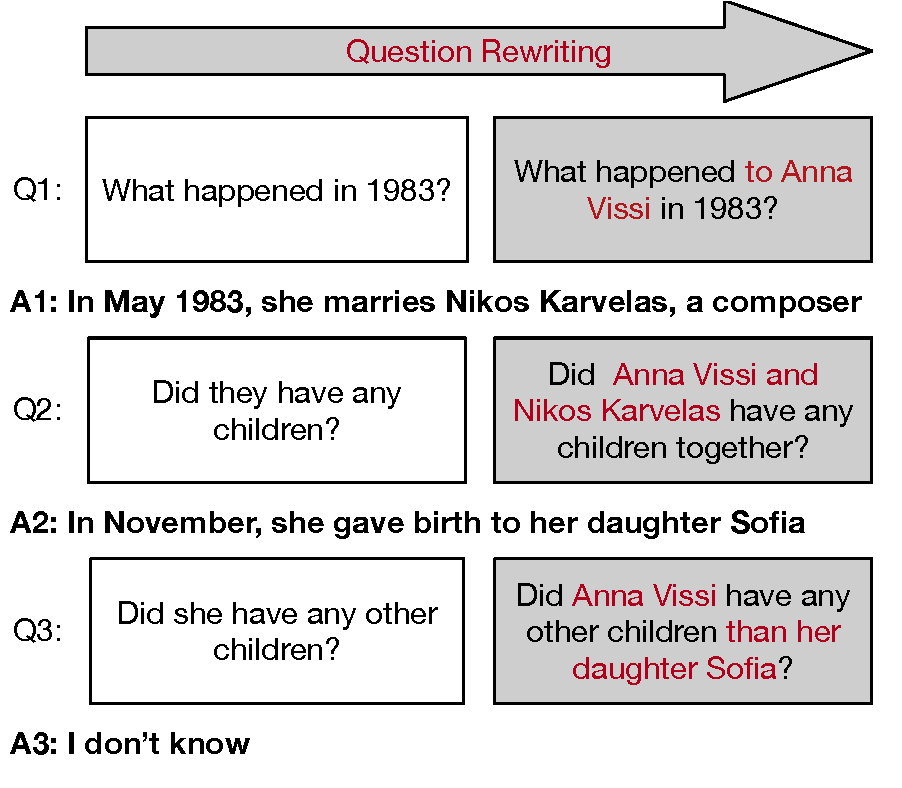
\includegraphics[width=.8\linewidth]{denis_proposal/figures/F1_OmniVersion.pdf}
	\caption{Question-in-context rewriting task. The input to each step
	is a question to rewrite given the dialog history which consists
	of the dialog utterances (questions and answers)  
	produced before the given question is asked. The output is an equivalent, context-independent paraphrase of the input question.}
	\label{fig:example_convo}
\end{figure}

Background Section~\ref{sec:qa} distinguishes between machine reading comprehension (\abr{mrc}) and the nascent area of conversational question answering (\abr{cqa}).  
%
However, we observe that \abr{cqa} questions can be rewritten as stand-alone \abr{mrc} questions and provide additional training data.  
%
We reduce challenging, interconnected \abr{cqa} examples to
independent, stand-alone \abr{mrc} to create
\name{}---\textbf{C}ontext \textbf{A}bstraction: \textbf{N}ecessary
\textbf{A}dditional \textbf{R}ewritten \textbf{D}iscourse---a new
dataset\footnote{\url{http://canard.qanta.org}} that rewrites
\abr{\quac}~\citep{choi2018quac} questions.
%
We crowd-source context-independent paraphrases of \abr{\quac}
questions and use the paraphrases to train and evaluate
question-in-context rewriting.
%
In the process, we observe the behavior of crowd users and the quality of their output.  
 %to simulate the interactive learning setup.

%\jbgcomment{``interactive learning setup'' doesn't make much sense to me}

%%%
%
%Other than being a pre-processing step for sequential
%question answering, the question-in-context paraphrasing task
%can be used for evaluating general models for dialogue understanding and
%sequence models for capturing long-term dependencies.
%As explained in Section~\ref{sec:data}, we made sure the reference
%paraphrases in our dataset are mostly copied spans from the
%conversation history, which makes BLEU~\citep{papineni2002bleu}
%a reliable measure for evaluating how different paraphrasing models
%perform on the task.

%%%%

Section~\ref{sec:data} constructs \name{}, a new dataset of
question-in-context with corresponding context-independent
paraphrases.
%
Section~\ref{sec:analysis} analyzes our rewrites (and the underlying
methodology) to understand the linguistic phenomena that make
\abr{cqa} and using crowd-sourcing for \textit{generation} difficult.


%%DENISTODO
%DONE\jbgcomment{The last sentence in above paragraph is devoid of content;
 % either cut or flesh out so that it wouldn't fit in any paper.}

%\input{denis_proposal/sections/automated/20-task-rewrite}

\begin{table}[t]
	\centering
	\begin{tabular}{l c}
	\textbf{	Characteristic }& \textbf{Ratio}\\
		\hline
		Answer Not Referenced & 0.98 \\
		Question Meaning Unchanged &  0.95 \\
		Correct Coreferences & 1.0 \\
		Grammatical English & 1.0 \\
		Understandable w/o Context & 0.90 \\
	\end{tabular}
    \caption{Manual inspection of 50 rewritten context-independent questions from \name{} suggests that the new questions have enough context to be independently understandable.}
    \label{tab:manualreview}
\end{table}

\section{Dataset Construction 
	\label{sec:data}}

We elicit paraphrases from human crowdworkers to make previously
context-dependent questions \textit{unambiguously} answerable.
%
Through this process, we resolve difficult coreference linkages and
create a pair-wise mapping between ambiguous and context-enriched
questions.
%
We derive \name{} from \abr{\quac}~\citep{choi2018quac}, a sequential
question answering dataset about specific Wikipedia sections.
%
\abr{\quac} uses a pair of workers---a ``student'' and a ``teacher''---to ask
and respond to questions.
%
The ``student'' asks questions about a topic based on only the title
of the Wikpedia article and the title of the target section.
%
The ``teacher'' has access to the full Wikipedia section and provides answers by selecting text that answers the question.
%
With this methodology, \abr{\quac} gathers 98k questions across 13,594 conversations.
%
We take their entire dev set and a sample of their train set and
create a custom JavaScript task in Mechanical Turk that allows
workers to rewrite these questions.
%
JavaScript hints help train the users and provides automated, real-time feedback.

We provide workers with a comprehensive set of instructions and task examples. 
We ask them to rewrite the questions in natural sounding English while preserving the sentence structure of the original question.  We discourage workers from introducing new words that are unmentioned
in the previous utterances and ask them to copy phrases when appropriate from the original question.
%
These instructions ensure that the rewrites only resolve
conversation-dependent ambiguities.
%
Thus, we encourage workers to create minimal edits; in
Section~\ref{sec:models}, we take advantage of this to use
\textsc{bleu} for evaluating model-generated rewrites.


We display the questions in the conversation one at a time, since the
rewrites should include only the previous utterance.  After a rewrite
to the question is submitted, the answer to the question is displayed.
The next question is then displayed.  This repeats until the end of
the conversation. The full set of instructions and the data collection
interface are provided in the appendix.

We apply quality control throughout our collection process, given the \textit{generation} issues noted in Background Section~\ref{sec:crowd}. 
%
During the task, JavaScript checks automatically monitor and warn
about common errors: submissions that are abnormally short
(e.g., `why'), rewrites that still have pronouns (e.g., `he wrote this album'),
or ambiguous words (e.g., `this article', `that').
%
Many \abr{\quac} questions ask about `what/who else' or ask for
`other' or `another' entity. For that class of questions, we ask
workers to use a phrase such as `other than', `in addition to', `aside
from', `besides', `together with' or `along with' with the appropriate
context in their rewrite.

We gather and review our data in batches to
screen potentially compromised data or low quality workers.
%
A post-processing script flags suspicious rewrites and workers who take and abnormally long or short time.
%
We flag about 15\% of our data.
%
\textit{Every} flagged question is manually reviewed by one of the
authors and an entire \textsc{hit} is discarded if one is deemed
inadequate.
%%DENISTODO
%DONE\jbgcomment{Who is doing this manual evaluation?}
%
We reject 19.9\% of submissions and the rest comprise \name{}.
%
Additionally, we filter out under-performing workers based on these
rejections from subsequent batches.
%
To minimize risk, we limit the initial pool of workers to those that
have completed 500 \abr{hit}s with over 90\% accuracy and offer competitive payment of \$0.50 per \abr{hit}.
% 
%Qualified workers are shown an extensive tutorial that walks them
%through the process upon joining the task.

We verify the efficacy of our quality control through manual review.
A random sample of fifty questions sampled from the final dataset is reviewed for desirable characteristics by a native English speaker in Table~\ref{tab:manualreview}.  Each of the positive traits occurs in 90\% or more of the questions.  Based on our sample, our edits retain grammaticality, leave the
question meaning unchanged, and use pronouns unambiguously.  There are rare occasions where workers use a part of the answer to the question being rewritten or where some of the context is left ambiguous.  These infrequent mistakes should not affect our models.
We provide examples of failures in Table~\ref{tab:rewriteexamples}.


\begin{table}[t]
  %\jbgcomment{Give the issues colors and then highlight the offending text with that color.  You can define your own arbitrary colors (examples in preamble).  Put the issue types in the caption (with top, middle, bottom as well as colors)}
 	\centering
    \begin{tabular}{l}
          \rowcolor{white}
		ORIGINAL: Was this an honest mistake by the media? \\
        \rowcolor{gray!25}
        REWRITE: Was the claim of media regarding Leblanc's room \textcolor{teal}{come to true?}\\
		\rowcolor{white}
		ORIGINAL: What was a single from their album? \\ 
		 \rowcolor{gray!25}
		 REWRITE: What was a single from \textcolor{violet}{horslips' \textit{album}}?  \\
          \rowcolor{white}
          ORIGINAL: Did they marry?  \\
	           \rowcolor{gray!25}
           REWRITE:   Did Hannah Arendt and Heidegger marry? \\
	\end{tabular}
        \caption{Not all rewrites correctly encode the context
          required to answer a question.  We take two failures to
          provide examples of the two common issues:
          \textcolor{teal}{Changed Meaning} (top) and
          \textcolor{violet}{Needs Context} (middle).  We provide an
          example with no issues (bottom) for comparison. }
	\label{tab:rewriteexamples}
\end{table}

We use the rewrites of \abr{\quac}'s development set as our test set
($5{,}571$ question-in-context and corresponding rewrite pairs) and use
a 10\% sample of \abr{\quac}'s training set rewrites as our
development set ($3{,}418$); the rest are training data ($31{,}538$).


\section{Dataset and Model Analysis}

\label{sec:analysis}

We analyze our discuss our datasets with automatic metrics. %after validating the reliability of our data (Section~\ref{sec:data}).
%
We compare our dataset to the original \abr{\quac} questions and to automatically generated questions by our models. 
%
Then, we manually inspect the sources of rewriting errors in the seq2seq baseline.
%
Further improvements for the \asr{} dataset and \name{} are possible.  

\subsection{Anaphora Resolution and Coreference}
%
Our rewrites are longer, contain more nouns and less pronouns, and have more  word types than the original data. 
%
Machine output lies in between the two human-generated corpora, but quality is difficult to assess. 
%
Figure~\ref{fig:bargraph} shows these statistics.  
%
We motivate our rewrites by exploring linguistic properties of our
data. 
%
Anaphora resolution and coreference are two core \textsc{nlp} tasks applicable to this dataset.%, in addition to the downstream tasks evaluated in Section~\ref{sec:expr}.  
%%DENISTODO
%\jbgcomment{avoid ``perform''.}


%QuAC provides many open ended questions.  20\% below human F1 level.  Long Tokens is a selling point.  Issue is context (CITE QuAC)


\begin{figure}[t!]
  \centering
	\includegraphics[width=.7\linewidth]{\figfile{length_and_ratio.pdf}}
	\caption{Human rewrites are longer, have fewer pronouns, and
          have more proper nouns than the original \abr{\quac} questions.
%
Rewrites are longer and contain more proper nouns than our Pronoun Sub
baseline and trained Seq2Seq model.}
	\label{fig:bargraph}
\end{figure}

%%DENISTODO
%\jbgcomment{This paragraph is very clunky.  As you go through, explain
 % why these numbers are they way they are.  E.g., ``\quac depends on
 % context; 54\% of \quac questions have a pronoun.''  Don't just give
  %numbers, give the {\bf why} you're mentioning these things.}

Pronouns occur in 53.9\% of \abr{\quac} questions.  Questions with pronouns are more likely to be ambiguous than those without any.   
%
 Only 0.9\% of these have pronouns that span more than one category
 (e.g., `she' and `his').  Hence, pronouns within a single sentence are likely unambiguous.  
%
 However, 75.0\% of the aggregate history has pronouns and the percentage of mixed category pronouns increase to 27.8\% of our data.  Therefore, pronoun disambiguation potentially becomes a problem for a quarter of the original data.  An example is provided in Table~\ref{tab:coreferenceexample}.
%

%
%Our automated baselines that replace pronoun create less proper
%nouns than human rewrites.
%
%Our task has over 10,000 questions that are likely to be
%interesting candidates for anaphora resolution.
%

 
\begin{table}
	\small
	\centering
	\begin{tabular*}{\linewidth}{l p{10cm}}

		{\bf Label} & {\bf Text} \\
          \hline
        
         QUESTION & How long did he stay there? \\
         \rowcolor{gray!25}
		REWRITE  & How long did Cito Gaston stay at the Jays? \\
		
		HISTORY & \parbox{10 cm}{\textit{Cito Gaston}
                           \newline  {\bf Q:} What did Gaston do after the world series? \dots \newline {\bf Q:} Where did he go in 2001? 
                           \newline {\bf A:} In 2002, he was hired by the Jays as special assistant to president and chief executive officer Paul Godfrey.} \\
	\end{tabular*}
	\caption{An example that had over ten flagged proper nouns in the history. Rewriting requires resolving challenging coreferences.}
	  
	\label{tab:coreferenceexample}
\end{table}

% \subsection{Types of Rewrites}

%I did my best to do that, spent a lot of time
%reading about different types of ellipsis
%and the other phenomena, but did not find enough
%resources to learn how those phenomna apply
%to dialogue. Did not take the risk of writing about
%something I do not understand. QuAC authors
%did not even cite any papers on that
%and the reviewers did not ask for it. yes, good to have, but 
%I do not know enough to do it.
% \jbgcomment{Still needs LINGUISTIC MOTIVATION on pronoun resolution
%  and context: what linguistic properties does this address (anaphora,
%  implicature, pragmatics, deictic expressions), and give
%  examples/citations}

Approximately one-third of the questions generated by our
pronoun-replacement baseline are within 85\% string similarity to our
rewritten questions.
%
That leaves two-thirds of our data that cannot be solved with pronoun resolution alone. 
%
%We notice several categories of rewrites: pronoun disambiguation, recipient specification, and question elucidation. 
%
%Our edits also look at coreference resolution.
%%DENISTODO
%\jbgcomment{``look at'' is vague, make clearer: why do you do this, how does this contrast with simple pronoun counting?}

\begin{comment}

\subsection{Model Analysis}
\label{sec:models}
\begin{table*}
\centering
\begin{tabular}{lp{6cm}p{8.5cm}}
	  \toprule
	 & \textbf{Seq2Seq output } & \textbf{Reference}\\
  \hline
1 & What did Chamberlain's men do? & What did Chamberlain's men do during the Battle of Gettysburg? \\
  %\hline
2 & How many games did Ozzie Smith win? & How many games did the Cardinals win while Ozzie Smith played? \\
  %\hline
3 & Did 108th get to the finals? & Did the US Women's Soccer Team get to the finals in the 1999 World Cup? \\
  %\hline
4 & Did Gabriel Batistuta reside in any other countries, besides touring in the Copa America? & Besides Argentina, did Gabriel Batistuta reside in any other countries? \\
%  \hline
5 & Did La Comedia have any more works than La Comedia 3? & Did Giannina Braschi have any more works than United States of Banana, La Comedia and Asalto al tiempo? \\
\bottomrule
\end{tabular}
\caption{Example erroneous rewrites generated by the Seq2Seq models
and their corresponding reference rewrites. The dominant
source of error is the model tendency to produce
short rewrites (Examples 1--3). Related entities (Copa America and Argentina in Example 4) distract the model. The model
struggles with listing multiple entities mentioned in different
parts of the context (Example 5).
}
  \label{tab:erranalysis}
\end{table*}

%\jbgcomment{Table / Example should be capitalized here}

By manually examining the predictions of the seq2seq model, we notice that the main source of errors is that the model tends to find a short path to completing the rewrites. That often results in \textit{under-specified questions} as in Example~1 in Table~\ref{tab:erranalysis}, \textit{question meaning change} as in Example~2 or \textit{meaningless questions} as in Example~3.

Another source of errors is having related entities mentioned in the context as 
Example~4 in Table~\ref{tab:erranalysis}, where the model confused ``Copa America''
with ``Argentina''. The model also struggles with listing multiple entities mentioned in different parts of the context. Example~5 in Table~\ref{tab:erranalysis}
show the output and the reference rewrites of the question \textit{``Did she have any more works than those 3?''}, where two of the three
	entities---``United States of Banana'', ``La Comedia'' and ``Asalto al tiempo''---are lost in the rewrite.  

\end{comment}


\subsection{Confidence in Data Quality}
\label{sec:discussion}


Confidences are a readily human-interpretable concept that may help build trust in the output of a system.
%
Transparency in the quality of up-stream content can lead to downstream improvements in a plethora of \textsc{nlp} tasks.

Exploring sequence models or alternate data representations may lead
to further improvement.  Including full lattices may mirror past results for machine
translation~\citep{sperber17emnlp} for the task of question answering.
%Phone-level approaches work in Chinese~\citep{lee2018odsqa}, but our phone
%models had lower accuracies than the baseline, perhaps due to a lack
%of contextual representation.
Using unsupervised approaches for \asr{}
\citep{wessel2004unsupervised,lee2009unsupervised} and training \asr{}
models for decoding \qb{} or Jeopardy! words are avenues for further
exploration.

\subsection{Can Question Answering Audio be Automated? }
\label{sec:conclusion}

Question answering, like many \textsc{nlp} tasks are impaired by noisy inputs.
%
Introducing \asr{} into a \abr{qa} pipeline corrupts the data. 
%
A neural model that uses the \asr{} system's confidence outputs and systematic forced decoding of words rather than unknowns improves  \textsc{qa} accuracy on \qb{} and Jeopardy! questions.  
%
Our methods are task agnostic and can be applied to other supervised \textsc{nlp} tasks.
%
Larger \textit{human-recorded} question datasets and alternate model approaches
would ensure spoken questions are answered accurately, allowing human
and computer trivia players to compete on an equal playing field.
%
Text-to-Speech technology can create a large dataset, but the unvarying pronunciation, speed, and voice---every single \abr{tts} voice is female---ultimately inhibits this approach from being a gold-standard.  
\section{Conclusion}
\label{sec:automated_conclusion}

In this chapter, we cover two types of low-cost dataset construction techniques: automation and generalist crowd-sourcing.  
%
The advantages of this method are cost and scalability, which is demanded by the current paradigm of neural models.   
%
This however comes at the expense of quality.  
%
A limitation of our past work in \textit{automation} is generalization: text-to-speech only has female voices and is consistently decoded, while the voices of real humans are decoded with large variations.  
%
Unseen data points are likely to confound a model trained on unnatural data.  
%
Additionally, automated data creation still depends on having quality source data, that often has to come from expert users.
%
In this project, we are able to record \textit{found} questions that were already written by Quizbowl experts.  
%
Writing hundreds of thousands of our questions would not have been tractable.
%
This suggests that expert design is necessary for automation, as discussed in Chapter~\ref{ch:contracat}.

A limitation of generalist \textit{crowd-sourcing} is the inability to automatically quality control \textit{generated} data.  
%
Our work requires \textit{manual} analysis of each sentence submitted by the crowd; this is time-intensive and subject to error.  
%
Additionally, it requires real-time task monitoring and user exclusion as otherwise malicious users can quickly contribute a large part of your crowd-sourced task.  
%
There is no full-proof way to ensure quality in tasks involving crowd-sourcing \textit{generation}.
%
However, this method seems to generate more diverse and lengthy sentences than a comparable automation technique.   
%
One way to handle the quality control issue is by using an expert for quality assessment, which we discuss in Chapter~\ref{ch:hybrid}. 

\chapter{Mixed Types of Users}
\label{ch:hybrid} 

%% abstract
\begin{abstract}
Trust is implicit in many online text conversations---striking up new
friendships, or asking for tech support. 
%
But trust can be betrayed through deception.
%
We study the language and dynamics of deception in the
negotiation-based game Diplomacy, where seven players compete for
world domination by forging and breaking alliances with each other.
%
Our study with players from the Diplomacy community gathers \totalnumber{}
messages annotated by the sender for their \textit{intended}
truthfulness and by the receiver for their \textit{perceived}
truthfulness.
%
Unlike existing datasets, this captures deception in long-lasting
relationships, where the interlocutors strategically combine truth
with lies to advance objectives.
%
A model that uses power dynamics and conversational contexts can
predict when a lie occurs nearly as well as human players.
\end{abstract}

As a dovetail between crowd-driven and expert-driven data sources, we propose an intermediate solution that pairs a person from the crowd with an expert.  
%
 This creates a verisimilitude of a customer, simulated by a worker from the crowd, interacting with a customer service agent, simulated by an actual professional customer service agent.  
%
The resulting dataset provides a stark contrast in the language generated by anonymous crowd workers and experts.\footnote{Denis Peskov,  Nancy Clarke,  Jason Krone,  Brigi Fodor,  Yi Zhang,Adel Youssef, and Mona Diab. Multi-domain goal-oriented dialogues(multidogo):  Strategies  toward  curating  and  annotating  large  scale dialogue data.  In Proceedings of  the 2019  Conference on  Empirical Methods in Natural Language Processing and the 9th International Joint Conference on Natural Language Processing (EMNLP-IJCNLP), pages 4518–4528, 2019.  \\
Peskov planned and implemented majority of crowd-sourcing tasks, supervised the data collection thereof, wrote part of the task guidelines,  performed data analysis, and wrote the majority of paper. 
}

\section{Introduction}


\begin{table*}[]
	\centering
	\small
	\begin{tabular}{p{.7 cm} p{7.8 cm} p{5 cm}}
		
		\textbf{Role}&  \textbf{ Turn } &  \textbf{Annotations} \\
		\hline
	
		A & Hey there! Good morning. You're connected to LMT Airways. How may I help you? & DA = \{ elicitgoal \} \\
		\rowcolor{gray!25}
		C & Hi, I wonder if you can confirm my seat assignment on my flight tomorrow? &  IC = \{ SeatAssignment \} \\
		A & Sure! I'd be glad to help you with that. May I know your last name please? &  DA = \{ elicitslot \} \\
				\rowcolor{gray!25}
		C &  My last name is Turker. & IC = \{ contentonly \}, 
		\newline SL = \{Name : Turker \} \\
		A & Alright Turker! Could you please share the booking confirmation number? & DA = \{ elicitslot \} \\
		\rowcolor{gray!25}
		C &  I believe it's AMZ685. & IC = \{ contentonly \}, 
		\newline SL = \{ Confirmation Number :  AMZ685 \} \\
		$\cdots$ & $\cdots$ & $\cdots$ \\
	\end{tabular}
	\caption{A segment of a dialogue from the airline domain annotated at the turn level.  This data is annotated with agent dialogue acts (DA), customer intent classes (IC), and slot labels (SL).  Roles C and A stand for ``Customer'' and ``Agent'', respectively.}
	\label{tab:TravelConvo}
\end{table*}



Modern Natural Language Understanding (NLU) frameworks for dialogues are by definition data hungry.  They require large amounts of training data representative of goal oriented conversations reflecting both context and diversity. But human responses in goal-oriented dialogues are less predictable than automated systems \citep{bordes2016learning}.  For example, ``Please do this'' cannot be interpreted without a broader context.  Only by seeing previous utterances, such as requests to book a flight on a specific day to a specific destination, can this task be performed.  Additionally, a single intent can be phrased in multiple ways depending on context; ``book my flight'', ``finalize my reservation'', ``Yes, the 6 pm one'' may all be referring to a flight-booking intent. Hence, entire conversations, rather than independent utterances, must be collected.  Such data is even more pertinent to modeling  \textsc{nlu} and related tasks as they require large, varied, and ideally human-generated datasets. Moreover, recent work \citep{dong2015multi,devlin2018bert} has shown the benefit of applying 
joint-training and transfer learning techniques to natural language processing tasks.
However, these approaches have yet to become widely used in dialogue tasks, due to a lack of large-scale datasets. Furthermore, the latest state of the art end-to-end neural approaches benefit from such training data even more so than past work on goal-oriented dialogues structured around slot filling~\citep{lemon2006isu,wang2013simple}.  One way to simulate data---and not risk releasing personally identifying information---for a domain is to use a Wizard-of-Oz data gathering technique, which requires that participants in a conversation fulfill a role \citep{kelley1984iterative}.  This approach has been used in popular public goal-oriented datasets: \textsc{dstc} and \multiwoz~\citep{williams2016dialog, budzianowski2018multiwoz}.

Conversations between people and automated systems occur with increasing frequency, especially in customer service.  Customers reach out to agents, which could be automated bots or real individuals, to achieve a domain-specific goal.  This creates a disparate conversation: agents are incentivized to operate within a set procedure and convey a patient and professional tone. In contrast, customers do not have this incentive. However, to date, the largest available multi-domain goal-oriented dialogue dataset assigns similar dialogue act annotations to both agents and customers \citep{budzianowski2018multiwoz}.   

To solve the aforementioned challenges, we present our efforts to curate, annotate, and evaluate a large scale multi-domain set of goal oriented dialogues.  The dataset is primarily gathered from workers in the crowd paired with professional annotators. The dataset elicited, \multidogo, comprises over 86K raw conversations of which 54,818 conversations are annotated at the turn level.  We investigate multiple levels of annotation granularity. We annotate a subset of the data on both turn and sentence levels. A turn is defined as a sequence of one or more speech/text sentences by a participant in a conversation. A sentence is a period delimited sequence of words in a turn. A turn may comprise one or more sentences. We do use the term  utterance to refer to a unit (turn or sentence, spoken or written by a participant).\footnote{ We acknowledge that the term utterance is controversial in the literature \citep{paretti18}} In our devised annotation strategy, we distinguish between dialogue speech acts for agents vs. customers. In \multidogo, the agents' speech acts   [\textsc{da}] are annotated with generic class labels common across all domains, while customer speech acts are labeled with  intent classes [\textsc{ic}]. Moreover, we annotate customer utterances with the appropriate slot labels [\textsc{sl}], which consist of the \textsc{sl} span and corresponding tokens with that \textsc{sl} tag. We present the strategies we use to curate and annotate such data given its contextual setting. We furthermore illustrate the efficacy of our devised approaches and annotation decisions against intrinsic metrics and via extrinsic evaluation, namely by applying neural baselines for \textsc{da}, \textsc{ic} and \textsc{sl} classification leveraging joint models. %% Nancy - do we annotate both customer and agent utterances with SL. I think just customer right ? 
\section{Existing Dialogue Datasets}


There are multiple existing goal-oriented dialogue collections generated by humans through Wizard-of-Oz techniques.  The Dialog State Tracking Challenge, \textit{aka} Dialog Systems Technology Challenge, (\textsc{dstc}) spans 8 iterations and entails the domains of bus timetables, restaurant reservations, and hotel bookings, travel, alarms, movies, etc. \citep{williams2016dialog}.  Frames \citep{asri2017frames} has 1369 dialogues about vacation packages.  \multiwoz contains 10,438 dialogues about Cambridge hotels and restaurants \citep{budzianowski2018multiwoz}. 
In addition to the datasets mentioned in Background Section~\ref{sec:dialog}, there are several dialogue datasets that specialize in a single domain. ATIS \citep{hemphill1990atis} comprises speech data about airlines structured around formal airline flight tables.  Similarly, the Google Airlines dataset purportedly contains 400,000 templated dialogues about airline reservations \citep{wei2018airdialogue}.\footnote{The Google Airlines dataset has not been released to date.}   %The Ubuntu Dialogue Corpus has over a million dialogues about Ubuntu technical support \citep{lowe2015ubuntu}.  %, and does more quality control than the latter of the two since we are intentionally eliciting this data, and not scraping existing data sources.  

On the other hand, Chit-chat style dialogues without goals have been popular since ELIZA and have been investigated with neural techniques \citep{weizenbaum1966eliza, li2016deep, li2017adversarial}.  
%
However, these datasets cannot be used for modeling goal-oriented tasks. 
%
Related dialogue dataset collections used for Sequential Question Answering rely on dialogue to answer questions, but the task is notably different from our use case of modeling goal oriented conversational AI, hence leading to different evaluation considerations \citep{choi2018quac,reddy2019coqa}.
\section{\multidogo Dataset Curation}

\textit{Generating} and \textit{annotating} a dataset of this scale requires extensive design prior to the task, collection, and post-task quality control.  

\begin{figure*}
	\centering
	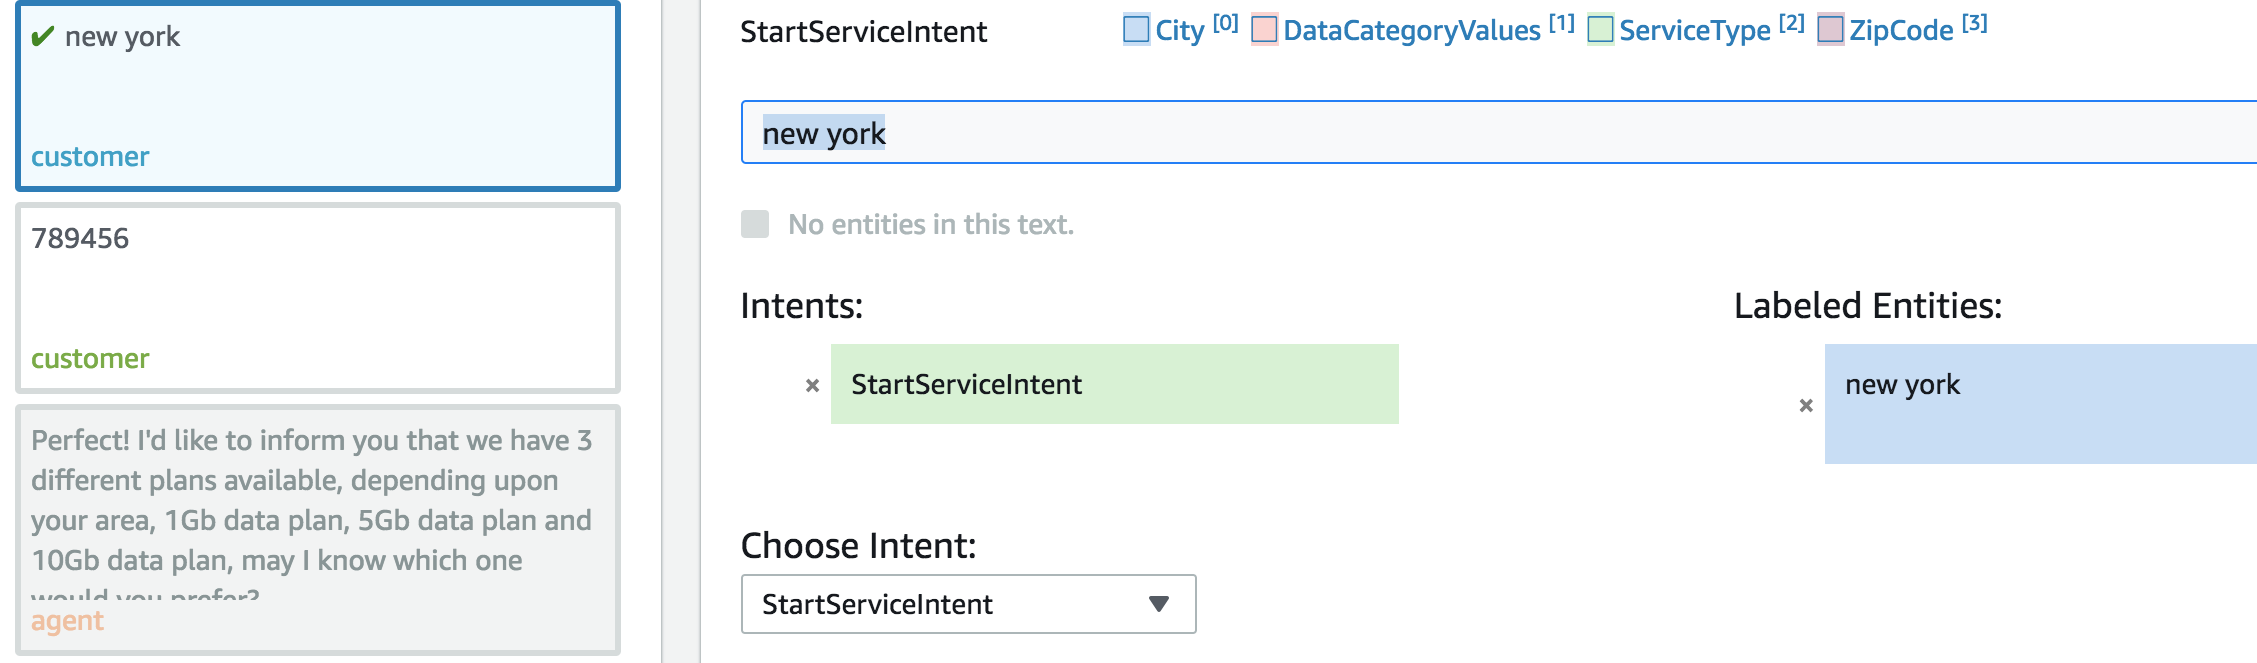
\includegraphics[width=\linewidth]{denis_proposal/sections/multidogo/figures/ic_sl-v3.png}
	\caption{Crowd sourced annotators select an intent and choose a slot in our custom-built Mechanical Turk interface.  Entire conversations are provided for reference.  Detailed instructions are provided to users, but are not included in this figure. Options are unique per domain.}%  There is a separate interface for data generation.}%%Nancy what is the data generation being referenced here?
	\label{fig:SlotAnnotation}
\end{figure*}
%\section{Design Decisions}\label{sec:motivation}

\subsection{Data Collection Procedure}
We employ both internal data associates, who we train,  and crowd-sourced workers from Mechanical  Turk  (MTurkers)  to  generate  conversational data using a Wizard-of-Oz approach. In each conversation, the data associates assumes the role of an agent while the MTurkers act as customers.  In an  effort  to  source  competent  MTurkers,  we  re-quire  that  each  MTurker  have  a  Human  Intelligence  Task  (HIT)  accuracy  minimum  of  90\%,  a location in the United States, and have completed a significant number of HITs in the past. To facilitate goal-oriented conversations between the customer  and  agent,  we  give  each  agent  a  prompt listing  the  supported  request  types  (dialog  acts)and pieces of information (slots) needed to complete each request.  We also specify criteria such as minimal conversation length, number of goals,number of complex requests, etc, to increase conversation diversity.  See Figure 2 for an example prompt. In addition, we explicitly request that neither agents nor customers use any personally identifiable information.  At an implementation level,we create a custom, web interface for the MTurkers and data associates that displays our instructions next to the current dialogue. This allows each participant to quickly refer to our guidelines with-out stopping the conversation.
Despite following a familiar wizard-of-oz elicitation procedure, and curating data for multiple domains in a fashion similar to previous data collection efforts such as \multiwoz, \multidogo comprises more varied domains, it is collected at an unprecedented scale, and it is curated with control over generating explicit biases in the conversations to allow for diverse conversation representation. To our knowledge this is a novel collection strategy as we explicitly guide/prod the participants in a dialogue to engage in conversations with specific biases such as intent change, slot change, multi-intent, multiple slot values, slot overfilling and slot deletion. 
For example, in the Fast Food domain, participants were instructed to pretend that they were ordering fast food from a drive-thru. After making their initial order, they were instructed to change their mind about what they were ordering:``I'd like a burger. No wait, can you make that a chicken sandwich?''. In the Financial domain, we asked participants to make sure that they requested multiple intents such as ``I'd like to find my routing number and check my balance.''\footnote{For a full list of conversational biases with examples, please see the appendix.}
%%NANCY lets add here a paragraph listing all the biases with a couple of examples and then a reference to the appendix for the exhaustive list
To that end, our collection procedure deliberately attempts to guide the dialogue flow to ensure diversity in dialogue policies.




\section{Data Annotation}
We discuss the \textit{annotation} needed for our dataset.  
%
Of particular interest, a direct comparison of using experts versus the crowd is made in in Section~\ref{sec:motivation}.

\subsection{Annotated Dialogue Tasks}
Our dataset has three types of annotation: Agent dialogue acts [\textsc{da}], customer intent classes [\textsc{ic}], and slot labels [\textsc{sl}].  
%
We intentionally decouple Agent and customer speech act tags into the categories \textsc{da} and \textsc{ic}, respectively, to produce more fine-grained speech act tags than past iterations of dialog datasets. 
%
Intuitively, agent \textsc{da}s are consistent across domains and more abstract in nature, since agents have a standard form of response. 
%
On the other hand, customer \textsc{ic}s are domain-specific and can entail reserving a hotel room or ordering a burger, depending on the domain.  
%
A conversation example with annotations is provided in Table~\ref{tab:TravelConvo}.



\textbf{Agent Dialogue Acts (\textsc{da})} Agent dialogue acts are the 
most straightforward of our annotation tasks. There are eight possible \textsc{da}s in all domains: 
{\textit{ElicitGoal, ElicitSlot, ConfirmGoal, ConfirmSlot, EndGoal, Pleasantries, Other}. The names are self-explanatory.  \textit{Elicit Goal/Slot} indicates that the agent is gathering information. \textit{Confirm Goal/Slot} indicates that the agent is confirming previously provided information.  The \textit{EndGoal} and \textit{Pleasantries} tags, identify non-task related actions. \textit{Other} indicates that the selected utterance was not one of the other possible tags. Agent dialogue acts are consistent across domains and are often abstract (e.g. ElicitIntent, ConfirmSlot).
	
	\textbf{Customer Intent Classes (\textsc{ic}):}
	Unlike Agent \textsc{da}, customer \textsc{ic} vary for each domain and are more concrete.  For example, the Airline domain has a ``BookFlight'' \textsc{ic}, Fast Food has an ``OrderMeal'' \textsc{ic}, and Insurance has an ``OrderPolicy'' \textsc{ic} in our annotation schema.  Customer intents can overlap across domains (e.g. OpeningGreeting, ClosingGreeting) and other times be domain specific (e.g. RequestCreditLimitIncrease, OrderBurger, BookFlight). 
	%% Nancy why didn't we make the greetings ICs as pleasantries similar to the DA
	
	
	{\textbf{Slot Labels (\textsc{sl}):}
	Slot Labeling is a task contingent on Customer Intent Classes.  Certain intents require that additional information, namely slot values, be captured. For instance, to open a bank account, one must solicit the customer's social security number.  Slots can overlap across intents (e.g. Name, SSN Number) or they can be unique to a domain-specific intent (e.g. CarPolicy). 
	
	
	\subsection{Data Annotation Procedure}
	Our annotators use a web interface, depicted in Figure \ref{fig:SlotAnnotation}, to select the appropriate intent class for an utterance out of a list of provided options. To annotate slot labels, our annotators use their cursors to highlight slot value character spans within an utterance and then select the corresponding slot label from a list of options. The output of this slot labeling process is a list of $\langle$slot-label, slot-value, span$\rangle$ triplets for each utterance.  
	\subsection{Annotation Design Decisions}
	\label{sec:motivation}
	
	\textbf{Decoupled Agents and Customers Label Sets}
	Agents and customers have notably different goals and styles of communication.  However, past dialogue datasets do not make this distinction at speech act schema level. Specificity is important for handling unique customer requests, but a relatively formulaic approach is required of agents across different industries.  Our distinction between the customer and agent roles creates training data for a bot that explicitly simulates agents. 
	
	\textbf{Annotation Unit Granularity: Sentence vs. Turn Level}
	An important decision, which is often under discussed, is the proper semantic unit of text to annotate in a dialogue.
	Commonly, datasets provide annotations at the turn level \citep{budzianowski2018multiwoz, asri2017frames, kvret}. 
	However, turn level annotations can introduce confusion for \textsc{ic} datasets, given multiple intents may be present in different sentences of a single turn. 
	For instance, consider the turn ``I would like to book a flight to San Francisco. Also, I want to cancel a flight to Austin."
	Here, the first sentence has the BookFlight intent and the second sentence has the CancelFlight intent. 
	An turn level annotation of this utterance would yield the multi-class intent (BookFlight, CancelFlight). 
	In contrast, a sentence level annotation of this utterance identifies that the first sentence corresponds to BookFlight while the second corresponds to CancelFlight.
	We annotate a subset our data, 2,500 conversation per domain for 15,000 conversations in total, at the sentence as well as turn level to access the impact of this design choice on downstream performance. The remainder of our dataset is annotated only at the turn level. %% Mona how do we motivate the fact that we choose to annotate at the turn level for the remainder of the dataset given this drops DA classification performance and turn and sentence level annotations are comparible in experimental  for IC SL. seems like sentence level would have been the right annotation unit here. 
	
	
	\begin{table}[t!]
		\small
		\centering
		\begin{tabular}{c  c  c }
			%\multicolumn{3}{c}{\textsc{isaa}} \\
			\textbf{Dialogue Act} &\textbf{ Intent Classes}& \textbf{Slot Labels} \\
			\hline
			0.701 & 0.728 & 0.695 \\
			\hline
		\end{tabular}
		\caption{Inter Source Annotation Agreement (\textsc{isaa}) scores quantifying the agreement of crowd sourced and professional annotations.}
		\label{ipa}
	\end{table}
	
	\textbf{Professional vs. Crowd-Sourced Workers for Annotation}
	For annotation, we compare and contrast professional annotators to crowd sourced annotators on a subset of data. Professional annotators assign \textsc{da}, \textsc{ic}, and \textsc{sl} tags to the 15,000 conversations annotated at both the turn and sentence level; statistics for these conversations are given in Table \ref{table:data}. In an effort to decrease annotation cost, we employ crowd source annotators via Mechanical Turk to label an additional 54,818 conversations rated as Good or Excellent quality during data collection. We provide statistics for this set of crowd annotated data in Table \ref{MultiDoGoStats}. To compare the quality of crowd sourced annotations against professional annotations, we use both strategies to annotate a shared subset of 8,450 conversations. 
	%
	We devise an Inter Source Annotation Agreement (\textsc{isaa}) metric to quantify the agreement of these crowd sourced and professionally sourced annotations. 
	%
	\textsc{isaa} is a relaxation of Cohen $\kappa$, intended to count partial agreement of multi-tag labels. 
	%
	\textsc{isaa} defines two sets of tags, $A$ and $B$, to be in agreement if there is at least one ``shared" tag in both $A$ and $B$. $A$ and $B$ reflect the majority labels agreed upon per source (professionals or crowd workers). Using \textsc{isaa} we find that crowd sourced and professional annotations have a substantial degree of shared annotations. We report \textsc{isaa} for the \textsc{da}, \textsc{ic}, and \textsc{sl} tasks in Table \ref{ipa}. 

\begin{table*}[t!]
	\centering
	\small
	\begin{tabular}{ l  c c c c }
		\textbf{Domain} & \textbf{Elicited} & \textbf{Good/Excellent} & \textbf{IC/SL} & \textbf{DA/IC/SL}\\
		\hline
		
		Airline & 15100&14205 & 7598& 6287 \\
		Fast Food & 9639& 8674&7712& 4507 \\
		Finance & 8814& 8160& 8002& 6704 \\
		Insurance &14262 &13400 & 7799& 7434 \\
		Media & 33321& 32231& 19877& 12891  \\
		Software &5562& 4924& 3830& 2753 \\
		\hline
		\textbf{Total} &\textbf{86698} & \textbf{81594}& \textbf{54818}& \textbf{40576} \\
	\end{tabular}
	\caption{Total number of conversations per domain: raw conversations Elicited; Good/Excellent is the total number of conversations rated as such by the agent annotators; (IC/SL) is the number of conversations annotated for Intent Classes and Slot Labels only; (DA/IC/SL) is the total number of conversations annotated for Dialogue Acts, Intent Classes, and Slot Labels.} %\citet{budzianowski2018multiwoz}.  We provide counts for the training data, except for \textsc{frames}, which does not %have splits.  Our number of unique tokens and slots can be attributed to us not relying on carrier phrases.}
	%%Mona modify this caption 
	\label{MultiDoGoStats}
\end{table*}

\subsection{Quality Control}\label{QC}
We institute three processes to enforce data quality.
During data collection, our data associates report on the quality of each conversation.
Specifically, the data associates grade the conversation on a scale from ``Unusable'', ``Poor", ``Good", to ``Excellent". They were provided with guidelines to help decide on the chosen rating such as coherence, whether the dialogue achieved the purported goal, etc.   To ensure high data quality we only utilize conversations with  ``Good" or ``Excellent" ratings in subsequent annotation. 

Secondly, each conversation is annotated at least twice. 
%
We resolve inconsistent annotations by selecting the annotation given by the majority of annotators per item. 
%
We calculate inter-annotator agreement with Fleiss' $\kappa$ and find ``substantial agreement'', according to the metric.\footnote{We use Fleiss' $\kappa$ unlike in the earlier profession/crowd worker comparison as we have more than two annotators for this task.}
%
Our annotators must pass a qualification test as well as maintain an on-going level of accuracy in randomly distributed test questions throughout their annotation. 
%
Third, we pre-process our data to remove issues such as duplicate conversations and improperly entered slot value spans. We refer readers to our discussion of pre-processing in Section~\ref{Baselines} for further detail.


\begin{table*}[t!]
	\centering
	\small
	\begin{tabular}{ l  c c c c c c}
		\textbf{Bias}& \textbf{Airlines} & \textbf{Fast Food}& \textbf{Finance} &\textbf{Insurance} & \textbf{Media}& \textbf{Software} \\
		\hline
		IntentChange & & 1443 & & & & \\
		MultiIntent & 2200 & 1913 & 1799 & 1061 & 607 & 2295 \\
		MultiValue & & 354& & & & \\
		Overfill & & & 1486 & 2763 & & \\
		SlotChange & 4207 & 2011& 2506 & 3321& 570 & 2085 \\
		SlotDeletion & & 333 & & & & \\
		\hline
		\textbf{Total} &6407 &6054 & 5791&7145 &1177 & 4380\\
		\hline
	\end{tabular}
	\caption{Number of conversations per domain collected with specific biases. Fast Food had the maximum number of biases. MultiIntent and SlotChange are the most used biases.} 
	%%Mona modify this caption 
	\label{biases}
\end{table*}

\subsection{Dataset Characterization and Statistics}

\multidogo dataset is more diverse by virtue of covering more domains, but more importantly, it is more controlled since it was curated rather than being scraped from existing data sources that are not necessarily synchronous (Ubuntu).
Table \ref{MultiDoGoStats} shows the statistics for \multidogo raw conversations harvested, rated as Excellent or Good, and annotated for \textsc{da}, \textsc{ic} and \textsc{sl}.  
%
Table~\ref{biases} shows the number of conversations per domain reflecting the specific biases used.




\multidogo is several orders of magnitude larger than  comparable datasets as reflected in nearly every dimension: the number of conversations, the length of the conversation, the number of domains, and the diversity of the utterances used. Table~\ref{Comparative} illustrates a comparative statistics to existing data sets.
\begin{table*}[t!]
	\centering
	\footnotesize
	\begin{tabular}{ l c c c c c a}
		\textbf{Metric} & \textbf{\textsc{dstc}} 2 & \textbf{\textsc{woz}2.0}  & \textbf{\textsc{M2M}} &   \textbf{\textsc{MultiWOZ}} & \textbf{\textsc{MultiDoGO}}\\
		\hline
		Number of Dialogues & 1,612 & 600 & 1,500 & 8,438 & 40,576 \\ %15,665 \\ %44,365\\
		Total Number of Turns & 23,354 & 4,472 & 14,796 & 115,424 & 813,834 \\ %249,167 \\ %964,513 \\
		Total Number of Tokens & 199,431 & 50,264  & 121,977 & 1,520,970 &  9,901,235\\%2,833,807 \\ %9,647,672\\
		Avg. Turns per Dialog & 14.49 &  7.45 & 9.86 & 15.91 & 20.06\\%16.56 \\ %21.74 \\
		Avg. Tokens Per Turn & 8.54 & 11.24& 8.24 & 13.18 & 12.16\\%11.37 \\ %10.00\\
		Total Unique Tokens & 986 & 2,142   & 1,008& 24,071 & 70,003\\%34,906 \\ %103,548\\ 
		Number of Unique Slots & 8 & 4  & 14 & 25 & 73\\%80 \\ %97 \\
		Number of Slot Values & 212 & 99  & 138 & 4,510 & 55,816\\%147,949 \\ %51,676\\
		Number of Domains & 1 & 1  & 1 & 7 & 6 \\
		Number of Tasks & 1 & 1  & 2 & 2 & 3 \\
		\hline
	\end{tabular}
	%% Jason, can you update this tabble to reflect the total harvested  %% MD
	\caption{\multidogo is several times larger in nearly every dimension to the pertinent datasets as selected by \citet{budzianowski2018multiwoz}.  We provide counts for the training data, except for \textsc{frames}, which does not have splits.  Our number of unique tokens and slots can be attributed to us not relying on carrier phrases.}
	%%Mona modify this caption 
	\label{Comparative}
\end{table*}


%\section{Dataset Summary and Statistics}
\begin{table*}[h!]
	\small
	\centering
	\begin{tabular}{l r r r r r r }
		%Domain & \# of Conv & Avg Utterances & Unique Intents & Unique Slots & Conv Quality & \abr{iaa}\\  
		%Domain & \#Conv & \#Turn & \#Utterance & Unique Intents & Unique Slots & Conv Quality & \abr{iaa}\\  
		\textbf{Domain} & \textbf{\#Conv} & \textbf{\#Turn }& \textbf{\#Turn/Conv} &\textbf{ \#Sentence} & \textbf{\#Intent} & \textbf{\#Slot} \\  
		\hline
		% without conv quality
		Airline & 2,500 & 39,616 & 15.8 (15) & 66,368 & 11 & 15    \\
		Fast Food & 2,500 & 46,246 & 18.5 (18) & 73,305 & 14 & 10   \\
		Finance & 2,500 & 46,001 &  18.4 (18) & 70,828 & 18 & 15    \\
		Insurance & 2,500 & 41,220 & 16.5 (16) & 67,657 & 10 & 9  \\
		Media & 2,500 & 35,291 & 14.1 (14) & 65,029 & 16 & 16     \\
		Software & 2,500 & 40,093 & 16.0 (15) & 70,268 & 16 & 15    \\
		
			\hline
	\end{tabular}
\caption{Data statistics by domain. Conversation length is shown in \textit{average (median)} number of turns per conversation. Inter-annotator agreement (\abr{iaa}) is measured with Fleiss' $\kappa$ for the three annotation tasks: Agent \abr{da} (\abr{da}), Customer \abr{ic} (\abr{ic}), and Slot Labeling (\abr{sl}).}
\label{table:data}
\end{table*}

\begin{table*}[h!]
	\small
	\centering
\begin{tabular}{l r r }
Domain & Turn-level \abr{iaa} & Sentence-level \abr{iaa} \\
\hline
Airline  & 0.514/0.808/0.802 & 0.670/0.788/0.771 \\
Fast Food  &  0.314/0.700/0.624 & 0.598/0.725/0.607 \\
Finance  &  0.521/0.827/0.772 & 0.700/0.735/0.714 \\
Insurance  &  0.521/0.862/0.848 & 0.703/0.821/0.826  \\
Media &  0.499/0.812/0.725 & 0.678/0.802/0.758 \\
Software &  0.508/0.748/0.745 & 0.709/0.764/0.698\\
	
			\hline
\end{tabular}
\caption{ Inter-annotator agreement (\abr{iaa}) is measured with Fleiss' $\kappa$ for the three annotation tasks: Agent DA (DA), Customer IC (IC), and Slot Labeling (SL).}	

\label{table:data}
\end{table*}
	
We provide summary statistics for the subset of our data annotated at both turn and sentence granularity in Table~\ref{table:data}.  This describes the total size of the data  per domain in number of conversations, turns, the unique number of intents and slots, and inter-annotator agreement (\abr{iaa}) for both turn and sentence level annotations. It is worth observing that the \textsc{da} annotations achieve a much higher \abr{iaa} in Sentence level annotations compared to Turn level annotation, most notably in the Fast Food domain. \textsc{ic} and \textsc{sl} annotations reflect a slightly higher \abr{iaa} in Turn level annotation granularity compared to Sentence level.  

	
\begin{figure}[t!]
	% By Jason: Replaced image with text box to make it easier to read the instructions
	%\includegraphics[scale=.44]{emnlp_2019/images/example_conversation.pdf}
	\centering
	\textbf{Agent Instructions}\par\medskip
	\small
	\fbox{\begin{minipage}{35em}
			Imagine you work at a bank.
			Customers may contact you about the following set of issues:
			checking account balances (checking or savings),
			transferring money between accounts, and
			closing accounts.\\
			
			\textbf{GOAL}: Answer the customer's question(s) and complete their request(s). \\
			
			For any request, you will need to collect at least the following information to be able to identify the customer: name, account PIN *or* last 4 digits of SSN. \\
			
			For giving information on balances, or for closing accounts, you will also need the last 4 digits of the account number. \\
			
			For transferring money, you will also need: last 4 digits of account to move from, last 4 digits of account to move to, and the sum of money to be transferred. \\
			
			Your customer may ask you to do only one thing; that's okay, but make sure you confirm you achieved everything the Customer wanted before completing the conversation.
			Don't forget to signal the end of the conversation (see General guidelines)
	\end{minipage}}
	\caption{Agents are provided with explicit fulfillment instructions. These are quick-reference instructions for the Finance domain. Agents serve as one level of quality control by evaluating a conversation between Excellent and Unusable.}  %Additional reference material is provided, but not pictured.}
	\label{Instructions}
\end{figure}

	\begin{table*}[t!]
	\footnotesize
	\centering
	\begin{tabular}{ c c  c c c  c c c  c c c }
		
		& & \multicolumn{3}{c}{Airline} & \multicolumn{3}{c}{Fast Food} & \multicolumn{3}{c}{Finance}   \\
		\hline
		Model & Annot & DA & IC & SL & DA & IC & SL & DA & IC & SL \\
		\hline
		MFC & S & 60.57 & 33.69 &	38.71 &	57.14 &	25.42 &	61.92 &	51.73 &	37.37 &	34.07 \\
		\lstm & S & 97.20 & 90.84 &	74.16 &	90.40 &	86.09 &	72.93 &	93.90 &	90.06 &	69.09 \\
		\elmo & S & \cellcolor{red!25}\textbf{97.32} & \cellcolor{red!25}\textbf{91.88} & \cellcolor{red!25}\textbf{86.55} & \cellcolor{red!25}\textbf{91.03} & \textbf{87.95} & \textbf{77.51} & \cellcolor{red!25}\textbf{94.07} & \textbf{91.15} & \textbf{77.36} \\
		\hline
		MFC & T & 33.04 & 32.79 &	37.73 &	33.07 &	25.33 &	61.84 &	36.52 &	38.16 &	34.31 \\
		\lstm & T & \textbf{84.25} & 89.15 &	75.78 &	\textbf{66.41} &	87.35 &	73.57 &	76.19 &	92.30 &	70.92 \\
		\elmo & T & 84.04 & \textbf{89.99} &	\textbf{85.64} &	65.69 &	\cellcolor{red!25}\textbf{88.96} &	\cellcolor{red!25}\textbf{79.63} &	\textbf{76.29} &	\cellcolor{red!25}\textbf{94.50} &	\cellcolor{red!25}\textbf{79.47} \\
		\hline
		& & \multicolumn{3}{c}{Insurance} & \multicolumn{3}{c}{Media} & \multicolumn{3}{c}{Software} \\
		\hline
		Model & Annot & DA & IC & SL & DA & IC & SL & DA & IC & SL \\
		\hline
		MFC & S & 56.87 &	38.37 &	53.75 &	57.02 &	30.42 &	82.06 &	58.14 &	33.32 &	53.96 \\
		\lstm & S & \cellcolor{red!25}\textbf{94.73} &	93.30 &	75.27 &	\cellcolor{red!25}\textbf{94.27} &	92.35 &	90.84 &	93.22 &	90.95 &	69.48 \\
		\elmo & S & 94.63 &	\textbf{94.27} &	\textbf{88.45} &	\cellcolor{red!25}\textbf{94.27} &	\textbf{93.32} &	\cellcolor{red!25}\textbf{93.99} &	\cellcolor{red!25}\textbf{93.66} &	\cellcolor{red!25}\textbf{92.25} &	\textbf{76.04} \\
		\hline       
		MFC & T & 36.39 &	39.42 &	54.66 &	29.90 &	31.82 &	78.83 &	36.79 &	33.78 &	54.84 \\
		\lstm & T & \textbf{75.37} &	94.75 &	76.84 &	\textbf{77.94} &	94.35 &	87.33 &	\textbf{83.32} &	89.78 &	72.34 \\
		\elmo & T & 75.34 &	\cellcolor{red!25}\textbf{95.39} &	\cellcolor{red!25}\textbf{89.51} &	77.81 &	\cellcolor{red!25}\textbf{94.76} &	\textbf{91.48} &	82.97 &	\textbf{90.85} &	\cellcolor{red!25}\textbf{76.48} \\
		\hline 
	\end{tabular}
	\caption{Dialogue act (\abr{da}), Intent class (\abr{ic}), and slot labeling (\abr{sl}) F1 scores by domain for the  majority class, \lstm, and \elmo baselines on data annotated at the sentence (S) and turn (T) level. Bold text denotes the model architecture with the best performance for a given annotation granularity, i.e. sentence or turn level. Red highlight denotes the model with the best performance on a given task across annotation granularities.}
	\label{icslresults}
\end{table*}


\begin{table*}[t!]
	\centering
	\scriptsize
	\begin{tabular}[\linewidth]{ c  c c  c c  c c  c c  c c  c c }
		& \multicolumn{2}{c}{Airline} & \multicolumn{2}{c}{Fast Food} & \multicolumn{2}{c}{Finance} & \multicolumn{2}{c}{Insurance} & \multicolumn{2}{c}{Media} & \multicolumn{2}{c}{Software} \\
		\hline
		A & Single & Joint & Single & Joint & Single & Joint & Single & Joint & Single & Joint & Single & Joint \\
		\hline
		S & 97.32 &	\cellcolor{red!25}\textbf{97.44} &	91.03 &	\cellcolor{red!25}\textbf{91.26} &	94.07 &	\cellcolor{red!25}\textbf{94.27} &	94.63 &	\cellcolor{red!25}\textbf{94.99} &	94.27 &	\cellcolor{red!25}\textbf{94.47} &	93.66 &	\cellcolor{red!25}\textbf{94.00} \\
		T & 84.04 &	\textbf{84.64} &	\textbf{65.69} &	65.35 &	\textbf{76.29} &	75.68 &	75.34 &	\textbf{75.89} &	77.81 &	\textbf{78.56} &	82.97 &	\textbf{83.76} \\
		\hline 
	\end{tabular}
	\caption{Joint training of ELMo on all agent DA data leads to a slight increase in test performance.  However, we expect stronger joint models that leverage transfer learning should see a larger improvement.  Bold text denotes the training strategy, i.e. single domain (Base) or multi-domain (Joint), with the best performance for a given annotation granularity. Red highlight denotes the strategy with the highest DA F1 score across annotation granularities.}
	\label{jointresults}
\end{table*}
\section{Dialogue Classification Baselines}\label{Baselines}
To establish baseline performance for the \multidogo dataset we pre-process, create dataset splits, and evaluate the performance of three baseline models for each domain. 

\textbf{Pre-processing:}
We pre-process the corpus of dialogues for each domain to remove duplicate conversations and utterances with inconsistent annotations. 
The most common source of inconsistent annotations in our dataset is imprecise selection of slot label spans by annotators, which results in sub-token slot labels. 
While much of this inconsistent data could likely be recovered by mapping each character span to the nearest token span, we drop these utterances to ensure these errors have no effect on our experimental results.
Our post-processed data is pruned to approximately 90\% of the original size. 
%\paragraph{Split Formation:}
We form splits for each domain at the conversation level by randomly assigning
70\% of conversations to train, 10\% to development, and 20\% to test.
Conversation level splits enable the application of contextual models to our dataset, as each conversation is assigned to a single split. However, our conversation level splits result in imbalanced intent and slot label distributions. %We considered balancing classes in the test set, but decide that maintaining a full conversation is integral to the task.  Hence certain intents, slots, and acts occur more than others.

\textbf{Models:}
We evaluate the performance of two neural models on each domain. The first is a bi-directional \lstm{}~\citep{hochreiter1997long} with GloVe word embeddings, a hidden state of size 512, and two fully connected output layers for slot labels and intent classes respectively. The second model, \elmo{}, is similar to the \lstm{}  architecture but it additionally uses pre-trained \elmo{}~\citep{Peters:2018} embeddings in addition to GloVe word embeddings, which are kept frozen during training.  We combine these \elmo{} and GloVe embeddings via concatenation.
%For brevity, we refer to the first model as \lstm and the second model as \elmo. 
As a sanity check, we also include a most frequent class (\abr{mfc}) baseline. The \abr{mfc} baseline assigns the most frequent class label in the training split to every utterance $u'$ in the test split for both \textsc{da} and \textsc{ic} tasks. To adapt the \abr{mfc} baseline to \textsc{sl}, we compute the most frequent slot label \abr{mfc}$(w)$ for each word type $w$ in the training set. Then given a test utterance $u'$, we assign the pre-computed, most frequent slot \abr{mfc}($w'$) to each word $w' \in u'$ if $w'$ is present in the training set. If a given word $w' \in u'$ is not present the training set, we assign the \textit{other} slot label, which denotes the absence of a slot, to $w'$. 
We use the AllenNLP \citep{Gardner2017AllenNLP} library to implement these models and evaluate our performance. 
%To access the impact of including previous turns as context, we experiment with a contextual version of the \lstm. This contextual \lstm encodes the tokens for the previous n-turns into a final hidden state that is concatenated with the hidden representations for the current turn at every time-step. 
%\subsection{Hyper-parameters}
We use the Adam optimizer \citep{kingma2014adam} with a learning rate of 0.001 to train the \lstm{} and \elmo{} models for 50 epochs, using batch sizes 256 and 128, respectively.  In addition, we employ early stopping on the validation loss with a tolerance of 10 epochs to prevent over fitting.

\textbf{Evaluation Metrics:}
We report micro F1 score to evaluate \textsc{da} and \textsc{ic} performance of our models. Similarly, we use a span based F1 score, implemented in the seqeval\footnote{https://github.com/chakki-works/seqeval} library,  to evaluate SL performance.
%This span based F1 score is more strict than a per token F1 score given it requires that start and end locations of the corresponding slot span match the ground truth annotations for a prediction to be considered correct. 

\subsection{Results}
\textbf{\abr{da}/\abr{ic}/\abr{sl} Results.} Table \ref{icslresults} presents the \abr{mfc}, \lstm{}, and \elmo{} results for each domain, on the subset of 15,000 conversations annotated at both the turn and sentence levels. In general for both granularities Turn and Sentence, both \lstm{}, and \elmo{} outperform \abr{mfc} significantly across all domains.  %One point of note for these results is the relatively high \textsc{da} performance of the majority class baseline. This performance is due to the large degree of imbalance with respect to dialogue acts in the dataset. In short, this metric should be interpreted literally as the proportion of the test split in each domain made up by the most common \textsc{da}. 
Relative to the \lstm, we find that \elmo{} obtains a modest increase in \textsc{ic} accuracy of 0.41 to 2.20 F1 points and a significant increase in \textsc{sl} F1 score on all domains. Concretely, \elmo{} boosts \textsc{sl} F1 performance by 3.16 to 13.17 F1 points. We see the biggest \textsc{sl} gains on the Insurance domain, where sentence level \elmo{} achieves the 13.17 point F1 gain and turn level \elmo{} achieves a 12.67 point F1 gain. Performance gains on the Airline domain are also large; here, \elmo{} increases sentence and turn level \textsc{sl} F1 score by 12.38 and 9.86 F1 points, respectively. 
%% Jason; add discussion of specific sl gains
Both \lstm{} and \elmo{} yield similar performance in terms of F1 score on \textsc{da} classification for which the difference in performance of these models is within one F1 point across all domains. In general, the Fast Food domain yields the overall lowest absolute F1 scores. Recall that Fast Food had the most diverse dialogues (biases) as per Table \ref{biases} and the lowest \abr{iaa} as per Table \ref{table:data}.
%n general we note that the results are in synch with the IAA. We note that there is 

\textbf{Sentence vs. Turn Level Annotation Units.}
Regarding the performance of the \lstm{} and \elmo{} models on sentence vs. turn level annotation units, our results suggest that turn level annotations increase the difficulty of the \textsc{da} classification task. This finding is evidenced by \textsc{da} performance of our models on the Fast Food domain, for which F1 score is up to 25 F1 points lower for turn level annotations than sentence level annotations. We believe the increased difficulty of turn level \textsc{da} relative to sentence level \textsc{da} is driven by a corresponding increase in the confusability of turn level dialogue acts. This assertion of greater turn level \textsc{da} confusability is supported by the lower inter annotator agreement (\abr{iaa}) scores on turn level \textsc{da}, which range from 0.314 to 0.521, relative to \abr{iaa} scores for sentence level \textsc{da}, which range from 0.598 to 0.709.  This experimental result highlights the importance of collecting sentence level annotations for conversational \textsc{da} datasets. Somewhat surprisingly, our models achieve similar \textsc{ic} F1 and \textsc{sl} F1 scores on turn and sentence level annotations. We hypothesize that the choice of annotation unit has a lesser impact on the \textsc{ic} and \textsc{sl} tasks because customer utterances are more likely to focus on a single speech act, whereas Agent utterances may be more complex in comparison and include a greater number of speech acts. 

	\textbf{Joint Training on Agent DA.} Agent \textsc{da} classification naturally lends itself to joint training, given agent \textsc{da}s are shared among all domains. To explore the benefits of multi-domain training, we jointly train an agent \textsc{da} classification model on all domains and report test results for each domain separately. These results are provided in Table~\ref{jointresults}. This straightforward technique leads to a consistent but less than one point improvement in F1 scores. We expect that more sophisticated transfer learning methods \citep{liu2017adversarial, howard2018universal} could generate larger improvements for these domains. 

Overall, our results demonstrate that there is still headroom for performance improvement, especially for the \textsc{sl} task, across all domains. Consequently, \multidogo should be a relevant benchmark for developing new state-of-the-art \abr{nlu} models for the foreseeable future.  



%Another promising direction, which we do not explore in this work, is to pre-train representations on \multidogo and then fine-tune these representations on a smaller, under resourced dataset. Pre-trained language models, such as \elmo \citep{Peters:2018} and BERT \citep{devlin2018bert}, demonstrate the value of using a self supervised language modeling objective to pre-train representations for natural language processing tasks. Yet the success of supervised pre-training on the ImageNet dataset \citep{deng2009imagenet} in the computer vision literature suggests that general purpose representations can be learned via a classification task. Therefore, we believe general purpose representations can be learnt via large-scale, supervised pre-training on \multidogo.  


\section{Conclusion}



We present \multidogo, a new Wizard-of-Oz dialogue dataset that is the largest human-generated, multi-domain corpora of conversations to date.  
%
The scale and range of this data provides a test-bed for future work in joint training and transfer learning.  
%
Moreover, our comparison of sentence and turn level annotations provides insight into the effect of annotation granularity on downstream model performance.

The data collection and annotation methodology that we use to gather \multidogo can efficiently scale across languages.  
%
Several pilot experiments aimed at collecting Spanish dialogues in the same domains have shown preliminary success in quality assessment. 
%
The production of a \abr{nlu} dataset with parallel data in multiple languages would be a boon to the cross-lingual research community. 
%
To date, cross-lingual \abr{nlu} research \citep{upadhyay2018almost, schuster2018cross} has relied on much smaller parallel corpora. 

By pairing crowd-sourced labor (Chapter~\ref{ch:unspecialized}) with experts (Chapter~\ref{ch:expert}), we balance the cost, diversity, and quality of these conversations in a scalable manner. 
%
We show that by adopting a modular annotation strategy, the crowds can reliably \textit{annotate} dialogues at a level commensurate with trained professional annotators. 
%
Without any oversight, our data would be just as large, but it could not be trusted.  

 However, there is a stark difference in quality of the \textit{generated} language between the crowd-sourced workers and the experts, in this case Amazon Customer Service agents.  
 %
 The crowd-sourced workers have a financial incentive to complete the task as quickly as possible and contribute sentences that are often prosaic, ungrammatical, or repeated.  
 %
 This begs the question, can we use only experts to create datasets?  And if so, will these datasets be rife with the same quality issues? 
\chapter{Using Experts for Design}

\label{ch:contracat}

Genuinely varied, realistic data is necessary to create models that are robust to minor variations. 
%
However, equally robust evaluation methodologies are important in ascertaining the quality of the data. 
%
Current methods focus on quantitative assessments that may inadvertently assess the \textit{annotation}, but not the \textit{generation}, quality of a dataset.  
%
Since most datasets are evaluated on the same types of data---\squad{} test data is comparable to the training data---the linguistic variation of a dataset is not readily captured by standard quantitative metrics like accuracy or \fone{}.
%
Furthermore, a model that has memorized several key answers upon which it is then tested is not necessarily \textit{learning}.
%
A raw analysis of data overlap appears this is at least partially a problem~\citep{lewis2020question}.    
%
Datasets meant to effectively and robustly evaluate trained datasets can determine how much of a problem this poses \textit{ex-post-facto}.  

As one solution to this limitation, Checklist~\citep{ribeiro2020beyond} created a task-agnostic methodology for testing NLP models.
%
We extend this work to a specific task: testing coreference~\citep{soon2001machine} in machine translation. %in Section~\ref{sec:propeval}.  
%
The dataset we create is \textit{designed} by experts: specifically native German and native English speakers, even if the methodology is \textit{automated}.
%
While a similar dataset of the same size could be created without knowledge of either language, the templates used as test data would prove be nonsensical or unnatural.  

\section{Meaningful Model Evaluation in Machine Translation}
\label{sec:propeval}

%Due to the intrinsic evaluation of many datasets, higher standards of evaluation would better understand the strength of machine learning models, and indirectly the data used to train them.
%

%


Machine translation is a classic \nlp{} task with immediate real-world application.
%
Its a complex task that requires diverse linguistic knowledge and data in multiple languages.
%
Classic datasets were often gathered through extensive collaboration with experts.
%
However, recent ones are often created through crowd-sourcing or automatic methods. 
%
Therefore, this is an area well-suited to our evaluation techniques.  

We focus on German-English coreference resolution as a representative task.  
%
The seemingly straightforward translation of the English pronoun \textit{it} into German requires knowledge at the syntactic, discourse and world knowledge levels for proper pronoun coreference resolution (\coref{}).
%
A German pronoun can have three genders, determined by its antecedent: masculine (\emph{er}), feminine (\emph{sie}) and neuter (\emph{es}).
%
The nuance of this work requires native knowledge of both English and German.  

Accuracy in machine translation is at an all-time high with the rise of neural architectures~\citep{wu2016googles}; but does accuracy alone suffice?  
%
Previous work~\citep{hardmeier2010modelling,miculicich-werlen-popescu-belis-2017-validation,mueller2018} proposed evaluation methods for specifically pronoun translation. 
%
This has been of special interest in context-aware neural machine translation (\nmt{}) models that are capable of using discourse-level information.
%
Despite promising results, the question remains: 
Are transformers \citep{vaswani2017attention} truly \textit{learning} this task, or are they exploiting simple heuristics to make a coreference prediction?
% 
To empirically answer this question, we propose extending ContraPro~\citep{mueller2018}---a contrastive challenge set for automatic English$\rightarrow$German pronoun translation evaluation\footnote{ContraPro is described in detail in Section~\ref{sec:contrapro}}---by making small adversarial changes in the contextual sentences.\footnote{Equal effort between Denis Peskov, Benno Krojer, Dario Stojanovski, and supervised by Alex Fraser. 2020. In International Conference on Computational Linguistics \\ Peskov is responsible for part of template design, selecting concrete nouns for the templates, paper writing, and the video.}

Our adversarial attacks on ContraPro show context-aware Transformer \nmt{} models can easily be misled by simple and unimportant changes to the input.
%
However, interpreting the results obtained from adversarial attacks can be difficult. 
%
In our case, trivial changes in language cause incorrect predictions, but both the changes and the prediction would not be noticed by somebody without a mastery of German.  
%
Positive results will show that \nmt{} uses brittle heuristics to solve \coref{}, since trivial changes in pronouns and nouns should not fool a coreference corpus like ContraPro.
%
However, modifying ContraPro alone will not test specific phenomena and will only demonstrate a broad dependence on heuristics.  

For this reason, we propose a new dataset, created from templates (Section~\ref{sec:template}), to systematically evaluate which heuristics are being used in coreferential pronoun translation.  
%
Inspired by previous work on \coref{}~\citep{raghunathan2010multi,lee2011stanford}, we will create templates tailored to evaluating the specific steps of an idealized \coref{} pipeline. 
%
We will call this collection \contracat{}, \textbf{C}ontrastive \textbf{C}oreference \textbf{A}nalytical \textbf{T}emplates. 
%
The construction of templates is controlled, enabling us to easily create large number of coherent test examples and provide unambiguous conclusions about the \coref{} capabilities of \nmt{}. 
%
While this methodology depends on automation, a technique called into question in Chapter \ref{ch:unspecialized}, the templates are written in collaborations between a native German speaker and native English speakers. 
%
Since automation is subject to quality control issues, this level of expertise is necessary if the adversarial dataset is to be reflective of actual language used by English and German speakers.
%
The procedure used in creating these templates can be adapted to many language pairs with little effort.
%
We also propose a simple data augmentation approach using fine-tuning. 
%
This methodology should not change the way \coref{} is being handled by \nmt{} and support the hypothesis that automated data techniques have limited applicability.  
%
We will publicly release a new dataset, ContraCAT, and the adversarial modifications to ContraPro.

ContraCAT applies only to coreference, but the investigation of heuristics is an important research direction in \nlp{}, that can quantify the issues noted with automatic and crowd-sourced datasets (Chapter~\ref{ch:unspecialized}), even if experts are unavailable ()Chapter~\ref{ch:hybrid}).
%
Heuristics perform well if there are underlying data limitations; this implies that the training data and the evaluation data resemble one another in superficial ones.
%
Therefore, exposing the brittleness in current datasets motivates the need for higher-quality evaluation data---to observe this limitation---and varied training data---to overcome it.  

We introduce coreference resolution as a task in Section~\ref{sec:mtbg}, the idealized coreference pipeline in Section~\ref{sec:mtbg}, and the transformer model in Section~\ref{sec:contracatmodel}.  
We discuss ContraPro in Section~\ref{sec:contrapro}, and explain our proposed templates in Section~\ref{sec:templates}.


\section{Why is Coreference Resolution Relevant?}
\label{sec:mtbg}


Evaluating discourse phenomena is an important first step in evaluating \abr{mt}.  
%
Apart from document-level coherence and cohesion, anaphoric pronoun translation has proven to be  an important testing ground for the ability of context-aware \nmt{} to model discourse. 
%
Anaphoric pronoun translation is the focus of several works in context-aware \nmt{}~\citep{bawden-etal-2018-evaluating,voita2018anaphora,stojanovski-fraser-2018-coreference,miculicich2018documentnmt,voita2019good,maruf2019selective}. 



\begin{table}[t]
	\centering
	\begin{tabular}{p{4cm} p{8cm}}
		\tikzmark{a} Start:  \newline Original sentence & The cat and the actor were hungry.  
		\newline
		It (?) was hungrier. \\
		\hline
		\tikzmark{b} Step 1: \newline  \stepone{} & The \textbf{cat} and the \textbf{actor} were hungry.  
		\newline
		It (?) was hungrier. \\
		\hline
		\tikzmark{c} Step 2: \newline  \steptwo{} & The cat and the actor were hungry. 
		\newline
		\textbf{It} was hungrier. \\
		\hline
		\tikzmark{d} Step 3: \newline \stepthree{} & Der Schauspieler und die Katze waren hungrig.
		\newline
		Er / \textbf{Sie} / Es   war hungriger.  \\
	\end{tabular}
	\begin{tikzpicture}[overlay, remember picture, yshift=.25\baselineskip, shorten >=2pt, shorten <=2pt, very thick]
	\draw [orange, ->] ({pic cs:a}) [bend right] to ({pic cs:b});
	\draw [orange, ->] ({pic cs:b}) [bend right] to ({pic cs:c});
	\draw [orange, ->] ({pic cs:c}) [bend right] to ({pic cs:d});
	
	\end{tikzpicture}
	
	\caption{A hypothetical \textsc{cr} pipeline that sequentially resolves and translates a pronoun.}
	\label{tab:corefpipeline}
\end{table}


The choice of an evaluation metric for \textsc{cr} is nontrivial. 
%
\textsc{bleu}-based evaluation is insufficient for measuring improvement in \textsc{cr}~\citep{hardmeier2012discourse} 
% and has led to custom variation
without carefully selecting or modifying test sentences for pronoun translation~\citep{voita2018anaphora,stojanovski-fraser-2018-coreference}.
%
Alternatives to \textsc{bleu} include $F_1$, partial credit, and oracle-guided approaches~\citep{hardmeier2010modelling,guillou-hardmeier-2016-protest,miculicich-werlen-popescu-belis-2017-validation}. 
%
However, \citet{guillou-hardmeier-2018-automatic} show that these metrics can miss important cases and propose semi-automatic evaluation. 
%
In contrast, our evaluation will be \textit{completely} automatic.  
%
We focus on scoring-based evaluation~\citep{sennrich-2017-grammatical}, which works by creating contrasting pairs and comparing model scores. 
%
Accuracy is calculated as how often the model chooses the correct translation from a pool of alternative incorrect translations.
%
This is an evaluation metric applicable for multiple forms of \textit{generated} \nlp{} data.

Our work is related to adversarial datasets for testing robustness used in  Natural Language Processing tasks such as  studying gender bias~\citep{zhao2018gender,rudinger2018gender,stanovsky-etal-2019-evaluating}, natural language inference \citep{glockner-etal-2018-breaking} and classification \citep{wang2019natural}.
% wang2019 mentions works about synonym replacement 


\section{Do Androids Dream of Coreference Translation Pipelines?}
\label{sec:corefpipeline}

Imagine a hypothetical coreference pipeline that generates a pronoun in a target language, as illustrated in  Table~\ref{tab:corefpipeline}.
%
\textbf{First}, markables (entities that can be referred to by pronouns) are tagged in the source sentence (we restrict ourselves to concrete entities as concepts are incompatible with many verbs). 
%
Then, the subset of animate entities are detected, and human entities are separated from other animate ones (since \textit{it} cannot refer to a human entity).
%
\textbf{Second}, coreferences are resolved in the source language. 
%
This entails addressing phenomena such as world knowledge, pleonastic \textit{it}, and event references.  
%
\textbf{Third}, the pronoun is translated into the target language. This requires selecting the correct gender given the referent (if there is one), and selecting the correct grammatical case for the target context (e.g., accusative, if the pronoun is the grammatical object in the target language sentence).

%Thus, the
This idealized
pipeline would produce the correct pronoun in the target language. 
%
The coreference steps resemble the rule-based approach implemented in Stanford Core\textsc{nlp}'s CorefAnnotator~\citep{raghunathan2010multi,lee2011stanford}. 
%
However, \nmt{} models are unable to decouple
the individual steps
of this pipeline. 
%
We propose to isolate each of these 
steps through targeted examples.


\section{Model}
\label{sec:contracatmodel}

% \afcomment{TODO: fix ContraPRO to be ContraPro everywhere}
% \dscomment{Fixed, but keeping it as a reminder.}

We use a transformer model (Background Section~\ref{sec:seq2seq}) for all experiments and train a sentence-level model as a baseline.
%
The context-aware model in our experimental setup is 
a concatenation model~\citep{tiedemann2017neural} (\textsc{concat}) which is trained on a concatenation of consecutive sentences.
%
\textsc{concat} is a standard transformer model and it differs from the sentence-level model only in the way that the training data is supplied to it.\footnote{The training examples for this model are modified by prepending the previous source and target sentence to the main source and target sentence. 
	%
	The previous sentence is separated from the main sentence with a special token $<$SEP$>$, on both the source and target side. 
	%
	This also applies to how we prepare the ContraPro and \contracat{} data. 
	%
	We train the concatenation model on OpenSubtitles2018 data prepared in this way. 
	%
	We remove documents overlapping with ContraPro.}
% We incorporate contextual information into the model by concatenating consecutive sentences~\cite{tiedemann2017neural}.   
%




\section{Adversarial Attacks}
ContraPro, a contrastive challenge set, has limitations and our methodology for creating our own dataset addresses them.

\subsection{About ContraPro}
\label{sec:contrapro}

ContraPro is a contrastive challenge set  for English$\rightarrow$German pronoun translation evaluation. 
%
This dataset uses an  \textit{automated} approach, discussed in Chapter~\ref{ch:unspecialized}.
%
The automatic nature makes it subject to manipulation and prevents it from fully elucidating the limitations of neural coreference resolution. 
%
The set consists of English sentences containing an anaphoric pronoun ``it'' and the corresponding German translations (e.g., ``Give me your hand, ah, it's soft and hot, and it feels pleasant''$\overrightarrow{}$``Gib deine Hand, ah, sie ist weich und warm, und wohlig fühlt sie sich an.'').
%
It contains three contrastive translations, 
differing based on the gender of the translation of \textit{it}: \textit{er}, \textit{sie}, or \textit{es}.
%
The challenge set artificially balances the  amount of sentences where \textit{it} is translated to each of these three German pronouns.
%
The appropriate antecedent may be in the main sentence or in a previous sentence. 
%
For evaluation, a model needs to produce scores for all three possible translations, 
which are compared against ContraPro's gold labels.


We create automatic adversarial attacks on ContraPro that modify theoretically inconsequential parts of the context sentence before the occurrence of \emph{it}. 
%
Contrary to the expectation that a transformer model would be able to handle inconsequential priming, coreference accuracy degrades in all adversarial attacks.


\subsection{Adversarial Attack Generation}
\label{sec:templates}

Our three modifications are:

\begin{enumerate}[noitemsep]
	\item \textbf{Phrase Addition}: Appending and prepending phrases containing implausible antecedents:
	\vspace{.1cm}
	The Church is merciful \emph{\underline{but that's not the point}}. It always welcomes the misguided lamb.
	\vspace{.2cm}
	
	\item \textbf{Possessive Extension}: Extending original antecedent with possessive noun phrase:
	\vspace{.1cm}
	I hear \sout{her} \emph{\underline{the doctor's}} voice! It resounds to me from heights and chasms a thousand times!
	
	\vspace{.2cm}
	\item \textbf{Synonym Replacement}: Replacing original German antecedent with synonym of different gender (note: \emph{der Vorhang} (masc.) and \emph{die Gardine} (fem.) are synonyms meaning \emph{curtain}):
	
	The curtain rises. It rises. $\rightarrow$ \sout{Der Vorhang} \emph{\underline{Die Gardine}} geht hoch. \sout{Er} \emph{\underline{Sie}} geht hoch.
\end{enumerate}


Phrase Addition can be applied to all 12,000 ContraPro examples. 
%
The second and third attack can only be applied to 3,838 and 1,531 examples, due to the required sentence contingencies.  

\subsubsection{Phrase Addition}
%As shown in the example in Table~\ref{tab:attacks} 
This attack modifies the previous sentence
by appending phrases such as ``\dots{}\textit{but he wasn't sure}'' and also prepending phrases such as ``\emph{it is true}:\dots{}''.
%
A range of other simple phrases can be used, which we leave out for simplicity.  All phrases we tried provided lower scores.
%
These attacks either introduce a human entity or an event reference \textit{it} (e.g.,  \textit{``it is true''}) which are both not plausible antecedents for the anaphoric \textit{it}.
% In the case of  ``it is true:..." we also created attacks with  ``that is true" and attacks that append "...and it is true.". This measures the difference between ``it'' and ``that'' and the role of distances in anaphoric pronoun translation.  
% are these details important?

\subsubsection{Possessive Extension}
This attack introduces a new human entity by extending the original antecedent \emph{A} with a possessive noun phrase e.g., ``\textit{the woman's A}''. 
%
Only two-thirds of the 12,000 ContraPro sentences are linked to an antecedent phrase. Grammar and misannotated antecedents exclude half of the remaining phrases.
% For example regarding grammar, an antecedent in ContraPro such as \textit{this one/der hier}, cannot be extended with"\textit{the woman's\dots}".
% \dscomment{Is this necessary?}
We put \textsc{pos}-tag constraints on the antecedent phrases before extending them. 
% with possessive Noun Phrases. 
%
This filters our subset to 3,838 modified examples. 
%
Our possessive extensions can be humans (\textit{the woman's}), organisations (\textit{the company's}) and names (\textit{Maria's}).

\subsubsection{Synonym Replacement}
This attack modifies the original German antecedent by replacing it with a German synonym of a different gender. 
%
For this we first identify the English antecedent and its most frequent synset in WordNet \citep{miller1995wordnet}.
% , as a word sense disambiguation baseline. 
% no further reference about this
%
We obtain a German synonym by mapping this WordNet synsets to GermaNet \citep{hamp-feldweg-1997-germanet} synsets.
%
Finally, we modify the correct German pronoun translation to correspond to the gender of the antecedent synonym.

Approximately one quarter of the nouns in our ContraPro examples are found in GermaNet.  
In 1,531 cases, a synonym of different gender could be identified. 

Understanding the pronoun/noun relationship is needed to score well on the Synonym Replacement attack. This attack gets to the core of whether \nmt{} uses \coref{} heuristics instead.

We evaluate a random sample of 100 auto-modified examples as a quality control metric.  
%
There are 11 issues with semantically-inappropriate synonyms. 
%
Overall, in 14 out of 100 cases, the model switches from correct to incorrect predictions because of synonym-replacement.
%
Only 4 out of these 14 cases come from the questionable synonyms, showing that the drop in ContraPro scores is meaningful.

\begin{figure}[t!]
	\centering
	\includegraphics[width = \linewidth]{\figfile{F1.pdf}}
	\caption{Results with the sentence-level Baseline and \textsc{concat} on ContraPro and three adversarial attacks. 	
		The adversarial attacks modify the context, therefore the Baseline model's results on the attacks are unchanged and we omit them.  \textbf{Phrase}: prepending ``it is true: \dots''. \textbf{Possessive}:  replacing original antecedent \emph{A}  with ``Maria's \emph{A}''. \textbf{Synonym}: 
		replacing the original antecedent with different-gender synonyms.  Results for Phrase Addition are computed based on all 12,000 ContraPro examples, while for Possessive Extension and Synonym Replacement we only use the suitable subsets of 3,838 and 1,531 ContraPro examples. 
	}
	\label{fig:contrapro}
\end{figure}



\subsubsection{Evaluating Adversarial Attacks }


Intuitively, the adversarial attacks should not contribute to large drops in scores, since  no meaningful changes are being made.
%
If the model accuracy drops some, but not all the way to the original sentence-level baseline (Section~\ref{sec:contracatmodel}),  we can conclude that the concatenation model handles \coref{}, but likely with brittle heuristics.
%
If the model accuracy drops all the way to the baseline, then the model is memorizing the inputs.
%
These results can expose potential issues with the model, but it will still be difficult to pinpoint the specific problems. 
%
This reveals a larger issue with pronoun translation evaluation that cannot be addressed with simple adversarial attacks on existing general-purpose challenge sets. 
%
We propose \contracat{}, a more systematic approach that targets each of the previously outlined \coref{} pipeline steps with data synthetically generated from corresponding templates.

Automatic adversarial attacks offer less freedom than templates as many systematic modifications cannot be applied to the average sentence.
%
Thus, our \contracat{} templates will be built on the hypothetical coreference pipeline in Section~\ref{sec:corefpipeline} that target each of the three steps:
%
i) \stepone{}, ii) \steptwo{} and iii) \stepthree{}. 
%Step ii) (Coreference resolution) is targeted in more detail with additional sub-steps.
%
Our minimalistic templates draw entities from sets of animals, human professions~\citep{mccoy2019right},
foods, and drinks, along with associated verbs and attributes. 
%
We use these sets to fill slots in our templates. 
%
Animals and foods are natural choices for subject and object slots referenced by \emph{it}.
%
Restricting our sets to interrelated concepts with generically applicable verbs---all animals eat and drink---ensures semantic plausibility.
%
Other object sets, such as buildings, would cause semantic implausibility with certain verbs.  

\subsubsection{Template Generation}
\label{sec:template}

\begin{table}[t]
	\small
	\centering
	\begin{tabular}{p{4.5cm} p{9cm} }
		\textbf{Template Target} & \textbf{Example} \\
		\hline
		
		\noalign{\vskip 2mm} 
		\textbf{Priors} & \\
		Grammatical Role & The \emph{\textbf{cat}} ate the \emph{\textbf{egg}}. It (\cat{}/{\textit{egg}}) was big. \\
		Order & I stood in front of the \emph{\textbf{cat}} and the \emph{\textbf{dog}}. It (\cat{}/\textit{dog}) was big. \\
		Verb & Wow! She unlocked it. \\
		
		
		\noalign{\vskip 2mm} 
		\rowcolor{gray!25}
		\textbf{\stepone{}} & \\
		\rowcolor{gray!25}
		Filter Humans & The \textit{\textbf{cat}}  and the \textit{actress} were happy. However it (\cat{}) was happier.  \\
		
		\noalign{\vskip 2mm} 
		\textbf{\steptwo{}} & \\
		Lexical Overlap & The \textit{\textbf{cat}} ate the apple and the \textit{owl} drank the water. It (\cat{}/ \textit{dogFir}) ate the apple quickly. \\
		World Knowledge & The \textit{\textbf{cat}} ate the \textit{cookie}. It (\cat{}) was hungry. \\
		% \dscomment{Changed is hungry to was hungry for past tense consistency.}
		Pleonastic it & The \emph{cat} ate the \emph{sausage}. It was raining. \\
		Event Reference  & The \emph{cat} ate the \emph{carrot}. It came as a surprise. \\
		
		\rowcolor{gray!25}
		\noalign{\vskip 2mm} 
		\textbf{\stepthree{}} & \\
		\rowcolor{gray!25}
		Antecedent Gender &
		I saw a \textit{\textbf{cat}}. It(\cat{}) was big. 
		$\rightarrow$
		\newline
		Ich habe eine Katze gesehen. Sie (\cat{}) war gro{\ss}.
	\end{tabular}
	\caption{Template examples targeting different \coref{} steps and substeps. 
		% We used sets of associated nouns, i.e.,, \{dog, cat, pig, 
		%\} for Animals.
		% is this important here? In any case, it is not clear 
		For German, we create three versions with \emph{er}, \emph{sie}, or \emph{es} as different translations of \emph{it}.
		% For the German translation we created three versions of the template with \emph{er}, \emph{sie}, or \emph{es} as different translations of \emph{it}. 
		% For consistency with how our model is trained, sentences are separated by $<$SEP$>$.
		% moved this to Model
	}
	\label{tab:templates}
\end{table}

Our templates consist of a \emph{previous sentence} that introduces at least one entity and a \emph{main sentence} containing the pronoun \emph{it}.
%
We use contrastive evaluation to judge anaphoric pronoun translation accuracy for each template; we create three translated versions for each German gender corresponding to an English sentence, e.g., \textit{``The cat ate the egg. It rained.''} and the corresponding \textit{``Die Katze hat das Ei gegessen. \emph{Er/Sie/Es} regnete''}.
%
To fill a template, we only draw pairs of entities with two different genders, i.e., for animal $a$ and food $f$: gender($a$) $\neq$ gender($f$). 
%
This way we can determine whether the model has picked the right antecedent.

First, we will create templates that analyze priors of
the model for choosing a pronoun when no correct translation is obvious. 
%
Then, we will create templates with correct translations, guided by the three broad coreference steps.
% \dscomment{This paragraph may not be necessary. We can mention it in Priors.}
Table~\ref{tab:templates} provides examples for our templates.


% \subsubsection{Biases}
\subsubsection{Priors}

% \afcomment{I added the next sentence, I am bit concerned that people might get confused between the priors and the other templates, which are really different. In fact, even after adding this sentence I am still concerned about this.}

Our templates that test prior biases do not have a correct answer, but help to understand the model's biases.
%
We will expose three priors with our templates: i) grammatical roles prior (e.g., subject)
ii) position prior  (e.g., first antecedent) and iii) a general prior if no antecedent and only a verb is present.

For i), we will create a Grammatical Role template where both subject and object are valid antecedents. 
%

For ii), we will create a Position template where two objects are enumerated as shown in Table~\ref{tab:templates}. 
%
We will create an additional example where the entities order is reversed and test if there are priors for specific nouns or alternatively positions in the sentence.  

For iii), we will create a Verb template, expecting that certain transitive verbs trigger certain object gender choice. 
%
We will use 100 frequent transitive verbs and create sentences such as the example in Table~\ref{tab:templates}.


\subsubsection{Markable Detection with a Humanness Filter}
Before doing the actual \coref{}, the model will need to identify all possible entities that \textit{it} can refer to. 
%
We will construct a template that contains a human and animal which are in principle plausible antecedents, if not for the condition that \emph{it} does not refer to people. 
%
For instance, the model should always choose \emph{cat} in \textit{`` The \emph{actress} and the \emph{cat} are hungry. However \emph{it} is hungrier.''}. 

\subsubsection{Coreference Resolution}
Having determined all possible antecedents, the model will have to choose the correct one, relying on semantics, syntax, and discourse.
%
The pronoun \textit{it} can in principle be used as an \emph{anaphoric} (referring to entities), \emph{event reference} or \emph{pleonastic} pronoun \citep{loaiciga-etal-2017-disambiguating}.
%
For the anaphoric \textit{it}, we identify two major ways of identifying the antecedent: lexical overlap and world knowledge.  
%
Our templates for these categories are meant to be simple and solvable.  

\textbf{Overlap}: Broadly speaking the subject, verb, or object can overlap from the previous sentence to the main sentence, as well as combinations of them. 
%
This gives us five templates: i) subject-overlap ii) verb-overlap iii) object-overlap iv) subject-verb-overlap and v) object-verb-overlap.

%
We always use the same template for the context sentence, e.g., \textit{``The \textbf{cat} ate the apple and the \textbf{owl} drank the water.''}. 
%
For the object-verb-overlap we would then create the main sentence \textit{``It ate the apple quickly.''} and expect the model to choose \emph{cat} as antecedent.
%
To keep our overlap templates order-agnostic, we vary the order in the previous sentence by also creating \textit{``The \textbf{owl} drank the water and the \textbf{cat} ate the apple.''}

\textbf{World Knowledge}: \coref{} has been traditionally seen as challenging as it requires  world knowledge.
%
Our templates will test simple forms of world knowledge by using attributes that either apply to animal or food entities, such as \textit{cooked} for food or \textit{hungry} for animals.
%
We then evaluate whether the model chooses e.g., \emph{cat} in \textit{``The \textbf{cat} ate the cookie. It was hungry.''}
%
The model occasionally predicts answers that require world knowledge, but most predictions are guided by a prior for choosing the neuter \emph{es} or a prior for the subject.

% \bkcomment{should i do this?:}
% To see if the model exhibits world knowledge when the bias is not triggered as much, we construct a less natural but still plausible template: ``I looked at the \emph{cat} and the \emph{ice cream}. It had a sweet taste''. This leads to XXX.
% \dscomment{Commenting this for now.}

\textbf{Pleonastic and Event Templates}: For the other two ways of using \emph{it}, event reference and pleonastic-it, we again create a default previous sentence (\textit{``The \textbf{cat} ate the \emph{apple}.'')}. 
%
For the main sentence, we used four typical pleonastic and event reference phrases such as \textit{``It is a shame''} and \textit{``It came as a surprise''}.  
%
We expect the model to correctly choose the neuter \emph{es} as a translation every time.  

\subsubsection{Translation to German}
\label{gender_template}

After \coref{}, the decoder has to translate from English to German.
%
In  our contrastive scoring approach the translation of the English antecedent to German is already given.
%
However the decoder is still required to know the gender of the German noun to select between \emph{er}, \emph{sie} or, \emph{es}. 
%
We will test this with a list of concrete nouns selected from \citet{Brysbaert2014ConcretenessRF}, which we filter for nouns that occur more than $30$ times in the training data. 
%
This selects $2051$ nouns that are substituted for $N$ in: \textit{``I saw a $N$. It was \{big, small\}.''.}

\subsection{Results} \label{template_results}

The \textsc{concat} model becomes less accurate when actual \coref{} is required. 
%
It frequently falls back to choosing the neuter \emph{es} or preferring a position (e.g., first of two entities) for determining the gender.
%
For \emph{Markable Detection} the model always predicts the neuter \emph{es} regardless of the actual genders of the entities.

% When the model was tested to do \coref{} by looking at different types of overlaps, it failed to recognize the overlap and had instead a general preference for one of the two clauses. 
In the Overlap template, the model fails to recognize the overlap and has a general preference for one of the two clauses.
%
For instance in the case of verb-overlap, the model had a solid accuracy of $64.1\%$ if the verb overlapped from the first clause (\textit{``The cat ate and the dog drank. It ate a lot.''}) but a weak accuracy of $39.0\%$ when the verb overlapped from the second clause (\textit{``The cat ate and the dog drank. It drank a lot.''.}) 
%
The overall accuracy for the overlap templates is $47.2\%$, with little variation across the types of overlap. 
% \bkcomment{should i report overall score here or score for all 5 overlaps?}
% Surprisingly 
Adding more overlap, e.g., by overlapping both the verb and object (\textit{``It ate the apple happily''}), yields no improvement. 
%
Overall, the model pays very little attention to overlaps when resolving pronouns.
% \dscomment{not sure if this is good or not}

\begin{figure}[t!]
	\centering
	\includegraphics[width = \linewidth]{\figfile{F2.pdf}}
	\caption{Results comparing the sentence-level baseline to \textsc{concat} on Contra\abr{cat}.  Pronoun translation pertaining to World Knowledge and language-specific Gender Knowledge benefits the most from additional context.}
	\label{fig:templates}
\end{figure}


We also see weak performance for world knowledge. An accuracy of $55.7\%$ is slightly above the heuristic of randomly choosing an entity ($=50.0\%$).
% \dscomment{Check}
% This means there is some small world knowledge in the model, however not enough to solve the task.
With a strong bias for the neuter \emph{es}, the model has a high accuracy of $96.2\%$ for event reference and pleonastic templates, where \emph{es} is always the correct answer.
%
Based on the strong performance on the Gender template in Section~\ref{gender_template}, we conclude the model consistently memorized the gender of concrete nouns.
%
Hence, \coref{} mistakes stem from Step 1 or Step 2, suggesting that the model failed to learn proper \coref{}.



\begin{table}[ht]
	\small
	\centering	
	\begin{tabular}{l l}
		
		\multicolumn{2}{l}{\textbf{Antecedent-free augmentation}} \\
		\textit{Source} &
		You let me worry about that. $<$SEP$>$ How much you take for \underline{it}? \\
		\textit{Reference} &
		Lassen Sie das meine Sorge sein. $<$SEP$>$ Wie viel kostet \underline{er}? \\
		\textit{Augmentation 1} &
		Lassen Sie das meine Sorge sein. $<$SEP$>$ Wie viel kostet \underline{sie}? \\
		\textit{Augmentation 2} &
		Lassen Sie das meine Sorge sein. $<$SEP$>$ Wie viel kostet \underline{es}? \\
	\end{tabular}
	\caption{Examples of training data augmentations. The source side of the augmented examples remains the same.}
	\label{table:manual-examples-augmentations-main}
\end{table}

\section{Augmentation}
\label{sec:augment}

We present an approach for augmenting ContraPro to improve \textsc{cr}.    
%
Augmentation systematically expands the data to improve a model's robustness~\citep{kafle2017data}.
%
While challenging for \textsc{nlp},  we focus on a narrow problem which lends itself to easier data manipulation. 
%
Figure~\ref{fig:templates} shows that our model is capable of modeling the gender of nouns.
%
However, they also show a strong  prior for translating \textit{it} to \textit{es} and very little \coref{} capability.
%
Our goal with the augmentation is to alter the prior and test if this can improve \coref{} in the model.


We augment our training data 
and call it Antecedent-free augmentation (\textsc{afa}).
%
We identify candidates for augmentation as sentences where a coreferential \textit{it} refers to an antecedent not present in the current or previous sentence  (e.g., \textit{I told you before. $<$SEP$>$ \underline{It} is red.} $\rightarrow$ \textit{Ich habe dir schonmal gesagt. $<$SEP$>$ \underline{Es} ist rot.}).
%
We create augmentations by adding two new training examples where the gender of the German translation of ``it'' is modified 
(e.g., the two new targets are ``\textit{Ich habe dir schonmal gesagt. $<$SEP$>$ \underline{Er} ist rot.}'' and ``\textit{Ich habe dir schonmal gesagt. $<$SEP$>$ \underline{Sie} ist rot.}'').
The source side remains the same.
%
Table~\ref{table:manual-examples-augmentations-main} provides an additional example.
%
Antecedents and coreferential pronouns are identified using a \coref{} tool \citep{clark2016deep,clark-manning-2016-improving}.
%
We fine-tune our  already trained concatenation
model on a dataset consisting of the candidates and the augmented samples. 
%
As a baseline, we fine-tune on the candidates to confidently say that any potential improvements come from the augmentations. 


\subsection{Results}
Results for adversarial attacks on ContraPro and on our templates are independent and are discussed separately.  

\begin{figure}[ht!]
	\centering
	\includegraphics[width = \linewidth]{\figfile{F3.pdf}}
	\caption{Results comparing unaugmented and augmented \textsc{concat} on ContraPro and same 3 attacks as in Figure~\ref{fig:contrapro}. Results with non-augmented \textsc{concat} are the same as Figure \ref{fig:contrapro}.}
	\label{fig:augmentation-contrapro}
\end{figure}

\subsubsection{Adversarial Attacks}

\textsc{afa} provides large improvements, scoring 85.3\% on ContraPro (Figure~\ref{fig:augmentation-contrapro}).
%
The \textsc{afa} baseline  (fine-tuning on the augmentation candidates only) improves by 1.94\%, presumably because many candidates consist of coreference chains of ``it'' and the model learns they are important for coreferential pronouns. However, the improvement is small compared to \textsc{afa}. 
% translation. 



Prediction accuracy on \textit{er} and \textit{sie} is substantially increased, suggesting that the augmentation removes the strong bias towards \textit{es}. %Templates provide further evidence about this. 
%
Although, the adversarial attacks lower \textsc{afa} scores, 
in contrast to \textsc{concat}, the model is more robust and the accuracy degradation is substantially lower (except on the synonym attack).
% 
We experiment with different learning rates during fine-tuning and 
present results with the \textsc{lr} that obtain 
the  best  baseline ContraPro score.
%
Furthermore, \textsc{concat}  and \textsc{afa} obtain $31.5$  and $32.2$ \textsc{BLEU} on ContraPro, showing that this fine-tuning procedure, which is tailored to pronoun translation, does not lead to any degradation in overall translation quality.

\subsubsection{Templates}



The prior over gender pronouns is more evenly spread and not concentrated on \textit{es}.
%
This provides for a more even distribution on the Position and Role Prior template.

The augmented model has higher accuracy on markable detection, improving by $27.6\%$. 
%
Results for  the templates are in Figure~\ref{fig:augmentation-templates}.




\begin{figure}[!h]
	\centering
	\includegraphics[width = \linewidth]{\figfile{F4.pdf}}
	
	\begin{comment}
	\begin{tikzpicture}
	\begin{axis}[
	ybar,
	enlargelimits=0.15,
	legend style={at={(0.5,-0.18)},
	anchor=north,legend columns=-1},
	ylabel={Accuracy},
	symbolic x coords={Markable,Overlap,World,Pleonastic,Event,Gender},
	xtick=data,
	nodes near coords,
	nodes near coords align={vertical},
	height=5.2cm,
	width=12cm,
	bar width=0.5cm,
	]
	\addplot coordinates {(Markable,44) (Overlap,47) (World,57) (Pleonastic,100) (Event,96) (Gender,94)};
	\addplot coordinates {(Markable,71) (Overlap,51) (World,54) (Pleonastic,97) (Event,46) (Gender,94)};
	\legend{Non-Augment,Augment}
	\end{axis}
	\end{tikzpicture}
	\end{comment}
	% \caption{Augmentation improves \textsc{Concat}'s pronoun translations on ContraCAT.  We speculate that this is explained by a readjusting of the prior. }
	\caption{ContraCAT results with unaugmented and augmented \textsc{concat}. We speculate that readjusting the prior over genders in augmented \textsc{concat} explains the improvements on Markable and Overlap.}
	\label{fig:augmentation-templates}
\end{figure}

% Considering our augmentation approach, 
No improvements are observed on the World Knowledge template.
Pleonastic cases are still accurate, although not perfect as with \textsc{concat}. 
% The shift in prior distribution over pronouns causes a small number of mistakes. 
The Event template identifies a systematic issue with our augmentation. We presume this is due to the \coref{} tool marking cases where \textit{it} refers to events. 
%
We do not  apply any filtering and augment these cases as well,
thus creating wrong examples (an event reference \textit{it} cannot be translated to \textit{er} or \textit{sie}). 
%
As a result, the scores are significantly lower compared to \textsc{concat}. 
%
This issue with our model is not visible on ContraPro and the adversarial attacks results. In contrast, the Event template easily identifies this problem.

\textsc{afa} has a similar accuracy to the unaugmented baseline on the Gender template. 
%
However,
despite increasing by 3.8\%, results on Overlap are still underwhelming. 
%
Our analysis shows that augmentation helps in changing the prior. 
%
We believe this provides for improved \coref{} heuristics which in turn provide for an improvement in coreferential pronoun translation. 
%
Nevertheless, the Overlap template shows that augmented models still do not solve \coref{} in a fundamental way.


\section{Our Dataset in Context}

Addressing discourse phenomena is important for high-quality \abr{mt}.  
%
Apart from document-level coherence and cohesion, anaphoric pronoun translation has proven to be  an important testing ground for the ability of context-aware \nmt{} to model discourse. 
%
Anaphoric pronoun translation is the focus of several works in context-aware \nmt{}~\citep{bawden-etal-2018-evaluating,voita2018anaphora,stojanovski-fraser-2018-coreference,miculicich2018documentnmt,voita2019good,maruf2019selective}. 

\citet{bawden-etal-2018-evaluating} manually create such a contrastive challenge set for English$\rightarrow$French pronoun translation. 
%
ContraPro~\citep{mueller2018} follows this work, but creates the challenge set in an automatic way. 
%
We show that making small variations in ContraPro substantially changes the accuracy scores, precipitating our new dataset.


\citet{jwalapuram-etal-2019-evaluating} propose 
a model for pronoun translation evaluation 
trained on pairs of sentences
consisting of the reference and a system output with differing pronouns.
%
However, as \citet{guillou-hardmeier-2018-automatic} point out, this fails to take into account that often there is not a 1:1 correspondence between pronouns in different languages and that a system translation may be
correct
despite not containing the exact
pronoun in the reference, and incorrect even if containing the pronoun in the reference, because of differences in the translation of the referent.
%
Moreover, introducing a separate model which needs to be trained before evaluation adds an extra layer of complexity in the evaluation setup and makes interpretability more difficult. 
In contrast, templates can easily be used to pinpoint specific issues of an \nmt{} model.
%
Our templates follow previous work \citep{ribeiro-etal-2018-semantically,mccoy2019right,ribeiro2020beyond}
where similar tests are proposed for diagnosing \textsc{nlp} models.


\section{Recap}

In this work, we study how and to what extent \coref{} is handled in context-aware \nmt{}. 
%
This work shows that standard challenge sets can easily be manipulated with adversarial attacks that cause dramatic drops in performance, suggesting that \nmt{} uses a set of heuristics to solve the complex task of \coref{}. 
%
Attempting to diagnose the underlying reasons, we propose targeted templates which systematically test the different aspects necessary for \coref{}. 
%
This analysis shows that while some type of \coref{} such as pleonastic and event \coref{} are handled well, \nmt{} does not solve the task in an abstract sense. 
%
We also propose a data augmentation approach to see if simple data modifications can improve model accuracy. 
%
This methodology illustrates the dependence on data by models, and strengthen our claims that low-cost data generation techniques are approximating rather than \textit{solving} \nlp{} tasks.  
%
Having identified limitations in existing models, we argue for concrete data extensions for coreference resolution.  
%
This methodology---creating an adverserial dataset which tests the understanding of a model---can be applied to most \nlp{} tasks.  

This project introduces using an expert, in this case a native German speaker, in designing the dataset.  
%
However, we use templates rather than experts to scale the size of the dataset.
%
While we can create \textit{large} datasets, they end up (literally) formulaic.  
%
\textit{Solving} tasks like coreference, rather than just noting shortcomings of current datasets, will require building complex and nuanced datasets that allow a model to earn the edge cases of the task.  
%
These datasets will ultimately have to built by somebody familiar with the task:
can we use only experts for data generation?







\begin{comment}
\subsection{Implementation}

Imagine a hypothetical coreference pipeline that generates a pronoun in a target language, as illustrated in Table~\ref{tab:corefpipeline}.
%
\textbf{First}, markables (entities that can be referred to by pronouns) are tagged in the source sentence (we restrict ourselves to concrete entities as we wish to detect gender). 
%
Then, the subset of animate entities are detected, and human entities are separated from other animate ones (since \textit{it} cannot refer to a human entity).
%
\textbf{Second}, coreferences are then resolved in the source language. This entails handling phenomena such as world knowledge, pleonastic \textit{it}, and event references.  
%
\textbf{Third}, the pronoun is translated into the target language. This requires selecting the correct gender given the referent (if there is one), and selecting the correct grammatical case for the target context (e.g., accusative, if the pronoun is the grammatical object in the target language sentence).

%Thus, the
This idealized pipeline would produce the correct pronoun in the target language. The coreference steps resembles, e.g., the rules-based approach implemented in Stanford Core\textsc{nlp}'s CorefAnnotator~\citep{raghunathan2010multi,lee2011stanford}. However, \nmt{} models are currently unable to decouple each individual step of this pipeline. We propose to isolate each of these phenomenon through targeted examples.


\begin{table}[t]
	\small
	\centering
	\begin{tabular}{p{4cm} p{7cm} }
		\textbf{Template Target} & \textbf{Example} \\
		\hline
		
		\noalign{\vskip 2mm} 
		\textbf{Priors} & \\
		Grammatical Role & The \emph{\textbf{cat}} ate the \emph{\textbf{egg}}. It (egg or cat?) was big. \\
		Order & I stood in front of the \emph{\textbf{cat}} and the \emph{\textbf{dog}}. It (egg or cat?)) was big. \\
		Verb & Wow! She unlocked it. \\
		\hline
		
		\noalign{\vskip 2mm} 
		\textbf{\stepone{}} & \\
		
		Filter Humans & The \textit{\textbf{cat}}  and the \textit{actress} were happy. However it was happier.  \\
		\hline
		
		\noalign{\vskip 2mm} 
		\textbf{\steptwo{}} & \\
		Lexical Overlap & The \textit{\textbf{cat}} ate the apple and the \textit{owl} drank the water. It (cat) ate the apple quickly. \\
		World Knowledge & The \textit{\textbf{cat}} ate the \textit{cookie}. It (cat) is hungry. \\
		Pleonastic it & The \emph{cat} ate the \emph{sausage}. It was raining. \\
		Event Reference  & The \emph{cat} ate the \emph{carrot}. It came as a surprise. \\
		\hline
		
		\noalign{\vskip 2mm} 
		\textbf{\stepthree{}} & \\
		Antecedent Gender &
		I saw a \textit{\textbf{cat}}. It was big. 
		$\rightarrow$
		\newline
		Ich habe eine Katze gesehen. Sie (cat) \dots.
	\end{tabular}
	\caption{Template examples targeting different \coref{} steps and substeps. 
		% We used sets of associated nouns, i.e.,, \{dog, cat, pig, ...\} for Animals.
		% is this important here? In any case, it is not clear 
		For German, we create three versions with \emph{er}, \emph{sie}, or \emph{es} as different translations of \emph{it}.
		% For the German translation we created three versions of the template with \emph{er}, \emph{sie}, or \emph{es} as different translations of \emph{it}. 
		% For consistency with how our model is trained, sentences are separated by $<$SEP$>$.
		% moved this to Model
	}
	\label{tab:templates}
\end{table}

We will use a Transformer for all experiments and train a sentence-level model as a baseline.
%
We will incorporate contextual information into the model by concatenating consecutive sentences~\citep{tiedemann2017neural}.   
%
Training examples can be modified by prepending the previous sentence on the source and target side;  the previous sentence is separated from the main sentence with a special token $<$SEP$>$. 
%
This applies to ContraPro and ContraCAT. We will train a concatenation Transformer on OpenSubtitles2018 data prepared in this way. 
\end{comment}







\chapter{Using Experts as Participants}
\label{ch:expert}

%% abstract
\begin{abstract}
Trust is implicit in many online text conversations---striking up new
friendships, or asking for tech support. 
%
But trust can be betrayed through deception.
%
We study the language and dynamics of deception in the
negotiation-based game Diplomacy, where seven players compete for
world domination by forging and breaking alliances with each other.
%
Our study with players from the Diplomacy community gathers \totalnumber{}
messages annotated by the sender for their \textit{intended}
truthfulness and by the receiver for their \textit{perceived}
truthfulness.
%
Unlike existing datasets, this captures deception in long-lasting
relationships, where the interlocutors strategically combine truth
with lies to advance objectives.
%
A model that uses power dynamics and conversational contexts can
predict when a lie occurs nearly as well as human players.
\end{abstract}

Expert-created datasets can create datasets of a quality unachievable with generalists.  
%
This has a twofold benefit.
%
First, the accuracy, rather than the size, of the data allows the dataset to withstand the test of time.\footnote{The Penn Treebank~\citep{marcus1993building2}, which used graduate students in linguistics and spanned three years in the early 1990s, remains a staple of Computational Linguistics curriculum today}.
%
Second, tasks that require long-term commitment and complexity become possible.  
%
This result justifies the large investment of time, relationship-building, and money.  

As a contrast to the earlier crowd-sourced work, we create a deception dataset using only experts.
%
Participants---that are engaged in the task and  are appropriately compensated---both \textit{generate} and \textit{annotate} data in the span of a game that usually lasts over a month. 
%  
The resulting product is a gold standard of conversational \nlp{} data in terms of quality of language, diversity, and naturalness.\footnote{Denis Peskov, Benny Chang, Ahmed Elgohary, Joe Barrow, Cristian Danescu-Niculescu-Mizil, and Jordan Boyd-Graber. 2020. It Takes Two to Lie: One to Lie and One to Listen. In Proceedings of The Association for Computational Linguistics.\\
Peskov was responsible for designing the task, gathering the participants, running the games, building half the models, part of the data analysis, the visualizations, and the paper writing.}  
%
The conversations and annotations thereof would not be possible without experts from the community.

\section{Where Does One Find Long-Term Deception?}
\label{sec:intro}


A functioning society is impossible without trust.
%
In online text interactions, users are typically
trusting~\citep{shneiderman2000designing}, but this trust can be
betrayed through false identities on dating sites~\citep{toma2012lies},
spearphishing attacks~\citep{Dhamija2006WhyPW},
sockpuppetry~\citep{kumar_army_2017} and, more broadly, disinformation
campaigns~\citep{kumar_false_2018}.
%
Beyond such one-off antisocial acts directed at strangers, deception
can also occur in sustained relationships, where it can be
strategically combined with truthfulness to advance a long-term
objective~\citep{ Cornwell2001LoveOT, kaplar2004enigma}.

% Computational methods to understand and mitigate such anti-social behaviors have relied on the availability comprehensive datasets with gold-label annotations.
%%pre DNM
% A functioning society is impossible without trust.
% %
% In online text interactions, users are typically
% trusting~\citep{shneiderman2000designing}, but this trust can be
% betrayed through false identities on dating sites~\citep{toma2012lies},
% spearphishing attacks~\citep{Dhamija2006WhyPW}, and malicious
% rumors~\citep{Qazvinian2011RumorHI}.
% %
% Other violations of the online social compact such as spam
% e-mail have been mitigated through machine learning~\citep{graham-03}:
% find the problem and hide it from view.
% %
% However, this approach has not been applied to text deception because
% we lack large enough gold-standard deception datasets for training
% machine learning algorithms.
%\jbgcomment{Address Cristian's point that  this dataset is unique because it has sustained interactions, not just one-offs}

We introduce a dataset to study the strategic use of
deception in long-lasting relationships.
%
To collect reliable ground truth in this complex scenario, we design
an interface for players to naturally generate and annotate
conversational data while playing a negotiation-based game called
Diplomacy.
%
These annotations are done in \textit{real-time} as the players send
and receive messages.
%
While this game setup might not directly translate to real-world
situations, it enables computational frameworks for studying deception
in a complex social context while avoiding privacy issues.


%%% pre DNM
% This work rectifies this lacuna through a large dataset of
% creative messages annotated with deception---not just one-off messages but sustained interactions in a complex relationship.
% %
% We design an interface that allows users to naturally generate and
% annotate conversational data while playing the game called Diplomacy.
% %
% These annotations are done in \textit{real-time} on sent and received
% messages.  
% %
% Using a game allows us to avoid privacy issues in a research topic fraught with them.  
% %


%\jbgcomment{Troy is a good reference, but it isn't a text-based
  %interaction, so we should probably avoid it.  Reworked new
 % paragraph, but needs citeps.}

%DONE \jbgcomment{ This is good, but should probably be in related
%work with appropriate citations: court transcripts of perjury, emails
%from malicious hackers, and surreptitious user recordings.  But
%real-world data comes with real-world complications and privacy
%concerns. Therefore, we use an artificial construct that allows us to
%gather pertinent language data without any risk.}

%moved\jbgcomment{ Again, this is good, but probably should be later
%in a section about our formal definition:}

\begin{table}[t]
	\centering
	\small
	\begin{tabular*}{\linewidth}{p{10cm}p{2cm}p{2cm}}
		{\bf Message} & {\bf Sender's intention} & {\bf Receiver's percep.} \\
		\hline
		\noalign{\vskip 2mm} 
		\parbox{10 cm}{If I were lying to you, I'd smile and
                  say ``that sounds great.''  I'm honest with you
                  because I sincerely thought of us as partners.}
                & Lie & Truth \\
		\noalign{\vskip 2mm} 
		\rowcolor{gray!25}
		\parbox{10 cm}{You agreed to warn me of unexpected
                  moves, then didn't \dots You've revealed things to
                  England without my permission, and then made up a
                  story about it after the fact!}  & Truth & Truth \\
		\noalign{\vskip 2mm}
		\parbox{10 cm}{\dots I have a reputation in this hobby
                  for being sincere.  Not being duplicitous.  It has
                  always served me well. \dots If you don't want to
                  work with me, then I can understand that \dots} &
                Lie & Truth \\
		\noalign{\vskip 2mm} 
		\rowcolor{gray!25}
		\multicolumn{3}{c}{\textit{(Germany attacks Italy)}} \\ 
		\noalign{\vskip 2mm} 
		\parbox{10 cm}{Well this game just got less fun} & Truth& Truth \\
		\noalign{\vskip 2mm} 
		\rowcolor{gray!25}
		\parbox{10 cm}{For you, maybe} & Truth & Truth \\
	\end{tabular*}
	\caption{An annotated conversation between \player{Italy} (white) and \player{Germany} (gray) at a moment when their relationship breaks down.  Each message is annotated by the sender (and
          receiver) with its intended or perceived truthfulness; \player{Italy} is lying about \dots lying.}
	\label{tab:dialogexample}
\end{table}

After providing background on the game of Diplomacy and our intended deception annotations (Section~\ref{sec:diplo}),
%
we discuss our study (Section~\ref{sec:study}).
%
To probe the value of the resulting dataset, we develop lie prediction
models (Section~\ref{sec:models}) and analyze their results
(Section~\ref{sec:analysis}).
% Finally, we discuss this dataset within the deception literature
%(Section~\ref{sec:lit}) and discuss the relevance of studying
%deception in the context of long-lasting relationships
%(Section~\ref{sec:contribution}).



\section{Diplomacy}
\label{sec:diplo}


The Diplomacy board game places a player in the role of one of seven
European powers on the eve of World War I.
%
The goal is to conquer a simplified map of Europe by ordering armies
in the field against rivals.
%
Victory points determine the success of a player and allow them to build
additional armies; the player who can gain and maintain the highest
number of points wins.\footnote{In the parlance of Diplomacy games,
  points are ``supply centers'' in specific territories (e.g.,
  London).  Having more supply centers allows a player to build more
  armies and win the game by capturing more than half of the 34 supply
  centers on the board.}
%
The mechanics of the game are simple and deterministic: armies,
represented as figures on a given territory, can only move to adjacent
spots and the side with the most armies always wins in a disputed
move.
%
The game movements become publicly available to all players after the
end of a turn. \dpcomment{Chris M suggested adding sentence
  contrasting this with other information games}
%

Because the game is deterministic and 
everyone begins with an equal amount of armies, a player cannot win
the game without forming alliances with other players---hence the name
of the game: Diplomacy. \dpcomment{Chris M suggestion to inverse:
  Everyone begins with the same amount of armies, and because conflict
  is decided by superior force, a player cannot win the game without
  forming alliances}
%
Conquering neighboring territories depends on support from another
player's armies.
%
After an alliance has outlived its usefulness, a player often
dramatically breaks it to take advantage of their erstwhile ally's
vulnerability.
%
Table~\ref{tab:dialogexample} shows the end of one such relationship.
%
As in real life, to succeed a betrayal must be a surprise to the
victim.
%
Thus, players pride themselves on being able to lie \emph{and} detect lies.
%
Our study uses their skill and passion to build a dataset of deception
created by battle-hardened diplomats.
%
Senders annotate whether each message they write is an \alie{} and
recipients annotate whether each message received is a \slie{}.
%
Further details on the annotation process are in
Section~\ref{sec:interface}.
%
%The annotation reveals the sender's internal state, at the time the message is sent.  


\subsection{A game walk-through} 
\label{sec:walkthrough}

Figure~\ref{fig:full_game} shows the raw counts of one game
in our dataset.
%
But numbers do not tell the whole story.
%
We analyze this case study using rhetorical
tactics~\citep{cialdini2004social}, which \citet{oliveira2017dissecting}
use to dissect spear phishing e-mails and \citet{anand-11} apply to
persuasive blogs.
%
Mentions of tactics are in italic (e.g., \textit{authority}.
%; context for quotes in Appendix, Table~\ref{tab:persuasion}. 
%
For the rest of the paper, we will refer to players via the name of
their assigned \player{country}.
%

\begin{figure}[t]
	\centering
	\includegraphics[width=.75\linewidth, height = 13cm]{\autofig{game_lies.pdf}}
	\caption{Counts from one game featuring an \player{Italy}
          (green) adept at lying but who does not fall for others'
          lies.  The player's successful lies allow them to gain an
          advantage in points over the duration of the game.  In 1906,
          \player{Italy} lies to \player{England} before breaking
          their relationship.  In 1907, \player{Italy} lies to
          everybody else about wanting to agree to a draw, leading to
          the large spike in successful lies.}
	\label{fig:full_game}
\end{figure}

Through two lie-intense strategies---convincing \player{England} to betray
\player{Germany} and convincing all remaining countries to agree to a
draw---\player{Italy} gains control of the board.
%
\player{Italy}'s first deception is a plan with \player{Austria} to
dismantle \player{Turkey}.
%
\player{Turkey} believes \player{Italy}'s initial assurance of
non-aggression in 1901.
%
\player{Italy} begins by excusing his initial silence due to a rough day at
work, evoking empathy and \textit{likability}.
%
While they do not fall for subsequent lies, \player{Turkey}'s initial
gullibility cements Italy's first-strike advantage.
%
Meanwhile, \player{Italy} proposes a long-term alliance with \player{England}  against
\player{France}, packaging several small truths with a big lie.
%
The strategy succeeds, eliminating \player{Italy}'s greatest threat.

Local threats eliminated, \player{Italy} turns to rivals on the other
end of the map.
%
\player{Italy} persuades \player{England} to double-cross its
long-time ally \player{Germany} in a moment of \textit{scarcity}: if
you do not act now, there will be nowhere to expand.
%\jbgcomment{This didn't explain how this was scarcity, I added my best guess.}
%
\player{England} accepts help from ascendant Italy, expecting
\textit{reciprocity}.
%
However, \player{Italy} aggressively and successfully moves against
\player{England}.
%
The last year features a meta-game deception.
%
After \player{Italy} becomes too powerful to contain, the remaining four
players team up.
%
Ingeniously, \player{Italy} feigns acquiescence to a five-way draw,
individually lying to each player and establishing \textit{authority}
while brokering the deal.
%
Despite \player{Italy's} record of deception, the other players believe the
proposal (annotating received messages from \player{Italy} as truthful) and
expect a 1907 endgame, the year with the most lies.
%
\player{Italy}  goes on the offensive and knocks out \player{Austria}.
%
%\player{Italy}'s summary of the game in their own words is in the Appendix, Table~\ref{tab:userfeedback}.
%\jbgcomment{Give more explicit forward reference so that readers don't have to hunt.}

%\jbgcomment{Again, focus on who's lying}

%Cialdini seems to best citep and it's used by cybseceurity \jbgcomment{Link the examples to the literature.  Presumably these things have names, find out what those names are, and then citep a relevant paper.  Talk about how that's relevant for things like Phishing and social engineering.}

Each game has relationships that are forged and then riven.
%
In another game, an honest attempt by a strong \player{Austria} to woo an
ascendant \player{Germany} backfires, knocking \player{Austria} from the game.
%
\player{Germany} builds trust with \player{Austria} through a believed
fictional experience as a Boy Scout in Maine (\textit{likability}).
%
In a third game, two consecutive unfulfilled promises by an ambitious
\player{Russia} leads to a quick demise, as their subsequent excuses
and apologies are perceived as lies (failed \textit{consistency}).
%
In another game, \player{England}, \player{France}, and
\player{Russia} simultaneously attack \player{Germany} after offering
duplicitous assurances.
%
Game outcomes vary despite the identical, balanced starting board, as
different players use unique strategies to persuade, and occasionally
deceive, their opponents.
  
\subsection{Defining a lie}

%added citeps and additional definitions \jbgcomment{This needs to be fleshed out; need more citations.  E.g., citep things that look at fake profiles, reviews, etc. citep some of the alternate definitions of lies, talk about why we
  %don't use them.  }

Statements can be incorrect for a host of reasons: ignorance,
misunderstanding, omission, exaggeration.
%
\citep{gokhman2012search} highlight the difficulty of finding willful,
honest, and skilled deception outside of short-term, artificial
contexts~\citep{depaulo2003cues}.
%
Crowdsourced and automatic datasets rely on simple
negations~\citep{perez2017automatic} or completely implausible claims
(e.g., ``Tipper Gore was created in 1048'' from \citep{fever-18}).
%
While lawyers in depositions and users of dating sites will not
willingly admit to their lies, the players of online games are more
willing to revel in their deception.

We must first define what we mean by deception.
%
Lying is a mischaracterization; it's thus no surprise that a
definition may be divisive or the subject of academic
debate~\citep{gettier-63}.
%
We provide this definition to our users: ``Typically, when [someone]
lies [they] say what [they] know to be false in an attempt to deceive
the listener''~\citep{siegler1966lying}.
%
An orthodox definition requires the speaker to utter an explicit
falsehood~\citep{sep-lying-definition}; skilled liars can deceive with
a patina of veracity.
%
A similar definition is required for prosecution of perjury, leading
to a paucity of convictions~\citep{bogner-74}.
%
Indeed, when we ask participants what a lie looks like, they mention
evasiveness, shorter messages, over-qualification, and creating false
hypothetical scenarios~\citep{depaulo2003cues}.

\subsection{Annotating truthfulness}

\begin{figure}[t]
	\footnotesize
	\centering
	\includegraphics[width = \linewidth]{\figfile{Interface_v3.pdf}}
	\caption{Every time they send a message, players say whether
          the message is truthful or intended to deceive.  The receiver then
          labels whether incoming messages are a lie or not.  Here
          \player{Italy} indicates they believe a message from
          \player{England} is truthful but that their reply is not. }
        %\jbgcomment{Too small.  If this is to be included, make font bigger or zoom in to important regions.}
	\label{fig:interface}
\end{figure}


%\begin{figure*}[t]
%	\centering
%	\includegraphics[width=\linewidth]{\figfile{convo_example_v1.png}}
%	\caption{An example conversation from our messaging interface.  Users write messages and annotate them with thumbs up or thumbs down.  Germany has accused Italy of being an untrustworthy ally.}
%\end{figure*}


% don't think CHI comment relevant anymore \jbgcomment{\dpcomment{need help.  it's technically reliable, it looks like the game, and it's visually friendly.  How do I write this and how do I citep this a la CHI?}You can't just say ``easiest to use''.  Talk about what
	%made them easy to use with the language of CHI (affordances, idioms,
	%transfer effects, etc.).}

%The board and move placement is provided as Figure~\ref{fig:board}  
%Discord has been used for educational research in the past~\citep{lacher2018using}.

%done\jbgcomment{Distinction with prior work needs to be clearer.  That was	post-hoc; this is in the loop.  That focused on betrayal inferred from Talk about how that might affect people's patterns of lying, etc.  (Also, add citeps.)}

%\dpcomment{should all of below be a paragraph in the lit review instead}
%\jbgcomment{It doesn't have to be relegated to related work, but should be here like this.  Introduce this as you use the features.}

Previous work on the language of Diplomacy~\citep{niculaelinguistic}
lacks access to players' internal state and was limited to
\textit{post-hoc} analysis.
%
We improve on this by designing our own interface that gathers
players' intentions and perceptions in real-time
(Section~\ref{sec:interface}).
%
As with other highly subjective phenomena like
sarcasm~\citep{gonzalez-ibanez_identifying_2011,bamman_contextualized_2015},
sentiment~\citep{pang2008opinion} and framing~\citep{greene2009more},
the intention to deceive is reflective on someone's internal state.
%
Having individuals provide their own labels for their internal state
is essential as third party annotators could not accurately access
it~\citep{chang_dont_2020-1}.

Most importantly, our gracious players have allowed this language data
to be released in accordance with \abr{irb} authorized anonymization,
encouraging further work on the strategic use of deception in
long-lasting relations.\footnote{Data available at
  \url{http://go.umd.edu/diplomacy_data} and as part of ConvoKit
  \url{http://convokit.cornell.edu}.}

\section{Broader Applicability}

This differs from previous work that does not follow the expert-generated paradigm.  
%
The most prominent past work on Diplomacy in the \abr{nlp} community, \citep{niculaelinguistic}, did not collect their data and thus could not release it to the public.  
%
This hampers follow-up applications of the research; a believable Diplomacy-playing (and speaking) bot cannot be trained if the raw language data is redacted and shuffled.  
%
We believe this work can set a paradigm for work outside of Diplomacy, and even \abr{nlp}; the interface created for this project, as well as the pre and post-game user surveys can be modifying for any conversational task.  
%
Most importantly, building a relationship with data generators elevates the standard of the data and guarantees its liberal distribution.  
%
Further work is necessary in codifying data standards---Show Your Data, not only your Work\footnote{\citep{dodge2019show}}.

% intro
\section{Engaging a Community of Liars}
\label{sec:study}

This dataset requires both a social and technical setup: finding a
community that plays Diplomacy online and having them use a
framework for annotating these messages.

\subsection{Seamless Diplomacy Data Generation}
\label{sec:interface}

%RESOLVED jbgcomment{Popularity isn't a good reason to use discord.}

We need two technical components for our study: a game engine and a
chat system.
%The former can be found in an existing format through several
%websites: PlayDiplomacy, webDiplomacy, and Backstabbr.  After testing
%out the systems,
We choose Backstabbr\footnote{\url{https://www.backstabbr.com}} as an
accessible game engine on desktop and mobile platforms: players input
their moves and the site adjudicates game
mechanics~\citep{chiodini2020backstabbr}.
%
Our communication framework is atypical.
%
Thus, we create a server on Discord,\footnote{\url{https://www.discord.com}}
the group messaging platform most used for online gaming and by the
online Diplomacy community~\citep{techspot}.
%
The app is reliable on both desktop and mobile devices, free, and does
not limit access to messages.
%
Instead of direct communication, players communicate with a bot;
the bot does not forward messages to the recipient until the player
annotates the messages (Figure~\ref{fig:interface}).
%
In addition, the bot scrapes the game state from Backstabbr to sync
game and language data.

%\jbgcomment{Not fixed.  ``past research'', ``suggests'',
%``simplicity'', and ``desirable'' are vague, back it up with real
%citation that says something like: For low probability/stigma
%associated events, forced choice is better. Perhaps something useful
%to citep here:
%https://www.frontiersin.org/articles/10.3389/fpsyg.2017.00806/full }

%RESOLVD\jbgcomment{Discussing the binary forced-choice implies an
%alternative that is never actually stated; expand.}

%DENIS \jbgcomment{``given the difficulty of calibration between
%users'' is roundabout phrasing and requires backup.  Something like
%``calling a statement is a lie is difficult, and people would prefer
%degrees of deception.  We circumvent this through a forced choice''.
%Citations that back up both the difficulty, shading, etc. would help
%back this up.}

%RESOLVED\jbgcomment{Desireable requirement is vague.  What is desierable about it}

\jbgcomment{would like help in explicit claim, Ian't access brown
  paper anymore due to lack of eduroam; jbg: how are the results
  comparable, how do you know?  Needs greater specificity here.}

Annotation of lies is a forced binary choice in our experiment.
%
Explicitly calling a statement a lie is difficult, and people would
prefer degrees of deception~\citep{bavelas1990truths, bell1996liking}.
%
Thus, we follow previous work that views linguistic deception as
binary~\citep{buller-96,braun-16}.
%
Some studies make a more fine-grained distinction; for example,
\citet{vanswol-12} separate strategic omissions from blatant lies (we
consider both deception).
%
However, because we are asking the speakers themselves (and not
trained annotators) to make the decision, we follow the advice from
crowdsourcing to simplify the task as much as
possible~\citep{snow2008cheap, sabou2014corpus}.
%
\dpcomment{Wanted to avoid strong claim.  cartwright2019crowdsourcing
  finds that binary feels limited in a small experiment.  Removed this
  citep from the stronger claim \jbgcomment{Removed these citeps which
    invoke IRT, which we're not using: A comparison of binary forced
    choice to a Likert scale shows comparable results while limiting
    user bias~\citep{brown2011item, joubert2015comparison}.  }}
%
%
Long messages can contain both truths and lies, and we ask players to
categorize these as lies since the truth can be a shroud for their
aims.

%\jbgcomment{``Borders'' is vague, make this clearer.}

% Tangentially, our conversations are limited to pairwise interactions between players, as the flow and conversation and the annotation of received messages becomes complicated with multiple speakers in one thread.  
%% JBG 1209: Cutting, seems like it could invite complaint
% We poll users after completion of the study on the quality of their annotations.  More than 90\% of our users state that their annotations are more than 90\% accurate, on both sent messages and received messages.  
%\dpcomment{ Jordan cut this out.  This seems quite neat to me: to independently ask users, independent of their payment, if they took the task seriously.  Maybe write a blog post or something?	
%	We poll users after completion of the study on the quality of their annotations.  More than 90\% of our users state that their annotations are more than 90\% accurate, on both sent messages and received messages. }


\subsection{Building a player base}

%\jbgcomment{\dpcomment{how does one top that quote from the NYtTimes??? \jbgcomment{That is about the game itself, not about the community.  Something along the lines of groups of players gleefully calling themselves backstabbers, etc.}} Would be stronger with actual \emph{quote} that revels in lying / deception.}

\jbgcomment{Could you really find nothing about the size of the community?}

The Diplomacy players maintain an active, vibrant community through
real-life meetups and online play~\citep{AmericanLife2014,
  chiodini2020backstabbr}.
%
We recruit top players alongside inexperienced but committed players
in the interest of having a diverse pool.
%
Our experiments include top-ranked players and community leaders from online platforms,  grizzled in-person tournament players with over 100 past games, and board game aficionados.
%
These players serve as our foundation and during initial design helped
us to create a minimally annoying interface and a
definition of a lie that would be consistent with Diplomacy play.
%
Good players---as determined by active participation, annotation and
game outcome---are asked to play in future games.

In traditional crowdsourcing tasks compensation is tied
to piecework that takes seconds to complete~\citep{buhrmester2016amazon}.
Diplomacy games are different in that they can last a month\dots and
people already play the game for free.
%
Thus, we do not want compensation to interfere with what these players
already do well: lying.
%
Even the obituary of the game's inventor explains
\begin{quote}
  Diplomacy rewards all manner of mendacity: spying, lying, bribery,
  rumor mongering, psychological manipulation, outright intimidation,
  betrayal, vengeance and backstabbing (the use of actual cutlery is
  discouraged)''~\citep{nytimes}.
\end{quote}
%
Thus, our goal is to have compensation mechanisms that get people to
play this game as they normally would, finish their games, and put up
with our (slightly) cumbersome interface.
%
Part of the compensation is non-monetary: a game experience with
players that are more engaged than the average online player.

To encourage complete games, most of the payment is conditioned on
finishing a game, with rewards for doing well in the game.
%
Players get at least \$40 upon
finishing a game.
%
Additionally, we provide bonuses for specific outcomes: \$24 for
winning the game (an evenly divisible amount that can be split among
remaining players) and \$10 for having the most successful lies, i.e.,
statements they marked as a lie that others believed.\footnote{The lie
  incentive is relatively small (compared to incentives for
  participation and winning) to discourage an opportunistic player
  from marking everything as a lie. Games were monitored in real-time
  and no player was found abusing the system (marking more than
  $\sim$20\% lies). }
%
Diplomacy usually ends with a handful of players dividing the board among
themselves and agreeing to a tie.
%
In the game described in Section~\ref{sec:walkthrough}, the remaining
four players shared the winner's pool with Italy after 10 in-game
years, and Italy won the prize for most successful lies.


\begin{table}[t]
	\centering
	\begin{tabular}{ l l }
		\textbf{Category}            & \textbf{Value}  \\ 
		\hline			
		Message Count       &  13,132 \\ 
		\alie{} Count      &  591 \\ 
		\slie{} Count  	  & 566 \\
		Average \# of Words & 20.79 \\
	\end{tabular}
	\caption{Summary statistics for our train data (nine of twelve games).  Messages are long and only five percent are lies, creating a class imbalance.}
	\label{tab:summarystats}
\end{table}

\subsection{Data overview}


%
Table~\ref{tab:summarystats} quantitatively summarizes our data.
%
Messages vary in length and can be paragraphs long
(Figure~\ref{fig:wordfrequency}).
%
Close to five percent of all messages in the dataset are marked as
lies and almost the same percentage (but not necessarily the same
messages) are perceived as lies, consistent with the ``veracity
effect''~\citep{levine-99}.
%
In the game discussed above, eight percent of messages are marked as
lies by the sender and three percent of messages are perceived as lies
by the recipient; however, the messages perceived as lies are rarely
lies (Figure~\ref{fig:distribution}).





\begin{figure}
	\centering
	\includegraphics[width=.6\textwidth]{\autofig{LengthFrequency.pdf}}
	\caption{Individual messages can be quite long, wrapping deception in pleasantries and obfuscation.	\dpcomment{Cristian suggested removing}}
	\label{fig:wordfrequency}

\end{figure}

\subsection{Demographics and self-assessment}

%\jbgcomment{This is too long winded.  Say what's interesting/useful	and move the rest to supplement. }

%\jbgcomment{This title is not useful; make more precise}

%\jbgcomment{Make the demographic information tighter.  I would suggest rephrasing as: topic sentence (we collect general, demographic information), the median player is X (give footnote with details and point to plots), and consider themselves able to detect lies.}

%Working closely with users in this human user study allows to collect information that only the player can provide before and after the game. When users fill out the \textsc{irb} study consent form, we ask them to provide anonymous  demographic information.  We inquire about age bracket, gender, education level, English ability, and other languages spoken.  Additionally, we ask for Diplomacy experience and self-evaluation of lying and lie-detecting abilities.  All questions contain a ``Prefer Not to Answer'' response.  

We collect anonymous demographic information from our study
participants: the average player identifies as male, between 20 and 35
years old, speaks English as their primary language, and has played
over fifty Diplomacy games.\footnote{Our data skews 80\% male and 95\%
  of the players speak English as a primary language.  Ages range from
  eighteen and sixty-four.
%
Game experience is distributed across beginner, intermediate, and
expert levels.}
%
Players self-assess their lying ability before the study.
%
The average player views themselves as better than average at lying
and average or better than average at perceiving lies.
%The charts of interest can be seen in Figures~\ref{fig:questions1}.

 
 %, as seen in Figure~\ref{fig:questions2}.

%\jbgcomment{Everything in present tense}

%After the game, we ask users to describe their quality of annotation and provide insight into the game.  I
In a post-game survey, players provide information on whom
\textit{they} betrayed and who betrayed \textit{them} in a given game.
%
This is a finer-grained determination than the \textit{post hoc} analysis used in past work on
Diplomacy~\citep{niculaelinguistic}.
%
We ask players to optionally provide linguistic cues to their lying
and to summarize the game from their perspective.
%(examples in Appendix, Table~\ref{tab:userfeedback}).

\begin{table*}[t]
	\small
	
	%seems fine.  Not sure about Cassandra \jbgcomment{I think the labels were wrong here, so I adjusted.  Let me know if I screwed this up.}
	
	\begin{tabularx}{\textwidth}{r  l   X X}
		
		& &\multicolumn{2}{c}{\textbf{Receiver's perception}} \\
		
		& &  \textbf{Truth }&  \textbf{Lie} \\
		\toprule
		\multirow{2}{*}{ \rotatebox[origin=r]{90}{\textbf{Sender's intention}}} & \textbf{Truth}
		& \cellcolor{gray!25}\textbf{Straightforward}
		Salut! Just checking in, letting you know the embassy is open, and if you decide to move in a direction I might be able to get involved in, we can probably come to a reasonable arrangement on cooperation.  Bonne journee!
		& \textbf{Cassandra}
		I don't care if we target T first or A first. I'll let you decide. But I want to work as your partner. \dots I literally will not message anyone else until you and I have a plan. I want it to be clear to you that you're the ally I want.
		\\
		& \textbf{Lie}
		& \textbf{Deceived}
		You, sir, are a terrific ally. This was more than you needed to do, but makes me feel like this is really a long term thing! Thank you.
		&  \cellcolor{gray!25}\textbf{Caught}
		So, is it worth us having a discussion this turn? I sincerely wanted to work something out with you last turn, but I took silence to be an ominous sign.
		\\
		\bottomrule
	\end{tabularx}
	\caption{Examples of messages that were intended to be
          truthful or deceptive by the sender or receiver.  Most
          messages occur in the top left quadrant
          (Straightforward).  Figure~\protect{\ref{fig:distribution} shows the full distribution.  Both the intended and perceived properties
          of lies are of interest in our study. }}
	\label{tab:quadrant}
\end{table*}



\begin{figure}
	\centering
	\includegraphics[width=.6\textwidth]{\autofig{Distribution}}
	\caption{Most messages are truthful messages identified as the
          truth.  Lies are often not caught.
          Table~\protect{\ref{tab:quadrant}} provides an example from
          each quadrant. \dpcomment{Cristian questioned is to merge
            with above table, with raw count but without viz
            \jbgcomment{too late}}}
	\label{fig:distribution}
\end{figure}

\subsection{An ontology of deception}

Four possible combinations of deception and perception can arise from
our data.
%
The sender can be lying or telling the truth.
%
Additionally, the receiver can perceive the message as deceptive or
truthful.
%
We name the possible outcomes for lies as Deceived or Caught, and the
outcomes for truthful messages as Straightforward or
Cassandra,\footnote{In myth, Cassandra was cursed to utter true
  prophecies but never be believed.  For a discussion of Cassandra's
  curse \textit{vis a vis} personal and political oaths, see
  \citet{torrance-15}.} based on the receiver's annotation (examples
in Table~\ref{tab:quadrant}, distribution in
Figure~\ref{fig:distribution}).



% intro
\section{Detecting Lies}
\label{sec:models}

%\jbgcomment{Need better transition from previous section.}

We build computational models both to detect lies to better understand
our dataset.
%
The data from the user study provide a training corpus that maps
language to annotations of truthfulness and deception.
%
Our models progressively integrate information---conversational
context and in-game power dynamics---to approach human parity in
deception detection.

\subsection{Metric and data splits}

We investigate two phenomena: detecting what is \textit{intended} as a
lie and what is \textit{perceived} as a lie.
%
However, this is complicated because most statements are not lies:
less than five percent of the messages are labeled as lies in both the
\textit{\alie} and the \textit{\slie}
tasks (Table~\ref{tab:summarystats}).
%
Our results use a weighted \fone{} feature across truth and lie
prediction, as accuracy is an inflated metric given the class
imbalance~\citep{japkowicz2002class}.
%
We thus adopt an in-training approach~\citep{zhou2005training} where
incorrect predictions of lies are penalized more than truthful
statements.
%
The relative penalty between the two classes is a hyper-parameter
tuned on \fone{}.

Before we move to computational models for lie detection, we first
establish the \textit{human} baseline.
%
We know when senders were lying and when receivers spotted a lie.
%
Humans spot 88.3\% of lies.
%
However, given the class imbalance, this sounds better than it is.  
%
%Following the suggestion of  we are able to directly quantify the recipient's accuracy in detecting lies~\citept{levine-99}
Following the suggestion of \citep{levine-99}, we focus on the detection of lies, where humans have a 22.5 Lie \fone{}.


%\jbgcomment{in-training needs citep}

%;  this tuning is essential as an incorrect weight forces the model to predict exclusively lies or exclusively truths.
%\jbgcomment{``unreliable'' is vague; be more concrete}
%
%A most-frequent class estimator would get over 80\% accuracy by
%guessing ``Truth'' for each message given the imbalanced distribution
%of our class.
%
%In contrast, the \fone{} penalizes a model that refuses to learn the
%infrequent class.
%
%This imbalance is also a problem for training models.
%



%The appropriate weight of a lie is a hyper-parameter that is found through sweeps and ranges from 20 to 50 depending on the model.  This tuning is essential as an incorrect weight forces the model to predict exclusively lies or exclusively truths.    
%\jbgomment{Reframe to be specific to this task}
%

%\jbgcomment{Explain why not do the four-way task (not consistent with	what a user does).}
%
To prevent overfitting to specific games, nine games are used as training data, one is used for validation for tuning parameters, and two games are test data.  Some players repeat between games.
%
%We split the messages by game: messages from six games are used for training and messages from a seventh game are used as a held-out test set. 


\begin{figure*}[t]
	\centering
	\includegraphics{\autofig{results.pdf}}
	\caption{Test set results for both our \alie{} and \slie{}
          tasks.  We provide baseline (Random, Majority Class),
          logistic (language features, bag of words), and neural
          (combinations of a \textsc{lstm} with \textsc{bert}) models.
          The neural model that integrates past messages and power
          dynamics approaches human \fone{} for \alie{} (top).  For
          \alie{}, the human baseline is how often the receiver
          correctly detects senders' lies.  The \slie{} lacks such a
          baseline.}
	\label{fig:results}
\end{figure*}


\subsection{Logistic regression}

%\jbgcomment{We've tried out other models now, make sure we add them to paper.}

Logistic regression models, described in Background Section~\ref{sec:lr}, have interpretable coefficients which 
show linguistic phenomena that correlate with lies.
%
A \textit{word} that occurs infrequently overall but often in lies,
such as `honest' and `candidly', helps identify which messages are lies.

\citep{niculaelinguistic} propose linguistic {\bf \wordlist{}} that can predict
deception.  These are word lists that cover topics often used in
interpersonal communication---\textit{claims}, \textit{subjectivity},
\textit{premises}, \textit{contingency}, \textit{comparisons}, \textit{expansion}, \textit{temporal language associated with the future}, and \textit{all
  other temporal language}.
%\jbgcomment{Expand this so that you give intuition about the individual word lists, make it clear that they can see all of the words in the appendix}
%
The \wordlist{} word lists do not provide full coverage, as they focus
on specific rhetorical areas.
%
A logistic regression model with all word types as features further
improves \fone{}.

Power dynamics influence the language and flow of
conversation~\citep{danescu2012echoes, danescu2013computational,
  prabhakaran2013power}.
%
%Linguistic patterns in emails related to the fall of Enron tangentially address power~\citep{louwerse2010linguistic}. 
%
These dynamics may influence the likeliness of lying; a stronger
player may feel empowered to lie to their neighbor.
%
Recall that victory points (Section~\ref{sec:diplo}) encode how well a
player is doing (more is better).
%
We represent the power differential as the difference between the two players.
%
Peers will have a zero differential, while more powerful players will
have a positive differential with their interlocutor.
%
The differential changes throughout the game, so this feature encodes
the difference in the season the message was sent.
%
 For example, a message sent by an \player{Italy} with seven points to
 a \player{Germany} with two points in a given season would have a
 value of five.

%\jbgcomment{DENIS, need to finish. JBG Power imbalance should be introduced here and added as
 %LogReg feature; citep a relevant paper(s) as well }

\subsection{Neural}

%RESOLVED \jbgcomment{citep to back up the accuracy / interpretability tradeoff}

While less interpretable, neural models are often more accurate than
logistic regression ones~\citep{ribeiro2016should, belinkov2019analysis}.
%
We build a standard long short-term memory
network~\citep[\abr{lstm}]{hochreiter1997long}, described in Background Section~\ref{sec:seq2seq}, to investigate if word
sequences---ignored by logistic regression---can reveal lies.

Integrating message context and power dynamics improves on the neural baseline.  
%
A Hierarchical \textsc{lstm} can help focus attention on specific
phrases in long conversational contexts.
%
In the same way it would be difficult for a human to determine
\textit{prima facie} if a statement is a lie without previous context,
we posit that methods that operate at the level of a single message
are limited in the types of cues they can extract.
%
The hierarchical \textsc{lstm} is given the context of previous
messages when determining if a given message is a lie, which is akin
to the labeling task humans do when annotating the data.
%
The model does this by encoding a single message from the tokens, and
then running a forward \textsc{lstm} over all the messages. For each
message, it looks at both the content and previous context to decide
if the current message is a lie.
%
Fine-tuning \textsc{bert}~\citep{devlin2018bert} embeddings, introduced in Background Section~\ref{sec:seq2seq}, to this
model did not lead to notable improvement in \fone{}, likely due
to the relative small size of our training data.
%
Last, we incorporate information about power imbalance into this model.
%
This model approaches human performance in terms of \fone{} score by combining content with conversational context and power imbalance.  

%\jbgcomment{What about temporal features}






%\begin{figure}[t]
%	\centering
%	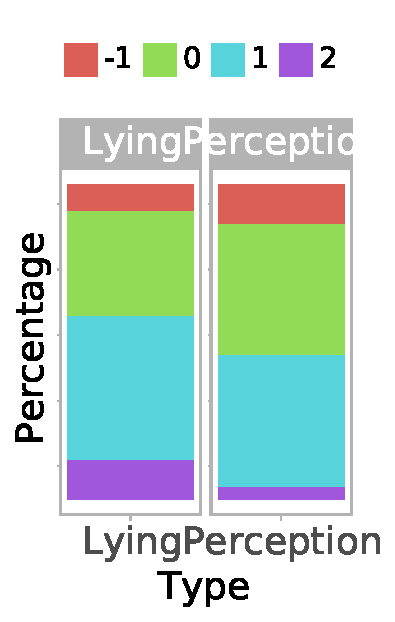
\includegraphics[width=\linewidth]{\autofig/DiploDemographics.pdf}
%	\caption{Most users self-assess themselves to be average or above at both lying and detecting lies.  Users assess themselves as better at perceiving lies than at telling them.}
%        \jbgcomment{I think this figure would be more efficient as normal text.  I'd cut.  Otherwise, change keys to something interpretable.}
%	\label{fig:questions2}
%\end{figure}

% intro
\section{Qualitative Analysis}
\label{sec:analysis}


\begin{table*}[t]
	\small
	\begin{tabularx}{\textwidth}{r  l   X X}
		& &\multicolumn{2}{c}{\textbf{Model Prediction}} \\
		
		& &  \textbf{Correct }&  \textbf{Wrong} \\
		\toprule
		\multirow{2}{*}{ \rotatebox[origin=r]{90}{\textbf{Player Prediction}}} & \textbf{Correct}
		& \cellcolor{gray!25}\textbf{Both Correct}
		Not sure what your plan is, but I might be able to support you to Munich.
		& \textbf{Player Correct}
		Don't believe Turkey, I said nothing of the sort. I imagine he's just trying to cause an upset between us. 
		\\
		& \textbf{Wrong}
		& \textbf{Model Correct}
		Long time no see. Sorry for the stab earlier. I think we should try to work together to stop france from winning; if we work together we can stop france from getting 3 more centers, and then we will all win in a 3, 4, or 5 way draw when the game is hard-capped at 1910.
		&  \cellcolor{gray!25}\textbf{Both Wrong}
		I'm considering playing fairly aggressive against England and cutting them off at the pass in 1901, your support for that would be very helpful.
		\\
                \bottomrule
	\end{tabularx}
	\caption{An example of an  \alie{} detected (or not) by both players and our best computational model (Context \textsc{lstm} + Power) from each quadrant.  Both the model and the human recipient are mostly correct overall (Both Correct), but they are both mostly wrong when it comes to specifically predicting lies (Both Wrong).}
        \jbgcomment{Once takeaway is finalized, needs to be recapitulated here.}
	\label{tab:predictionquadrant}
\end{table*}


%\begin{table*}
%\centering
%\begin{tabular}{lp{1cm}p{1cm}p{12cm}}
%	  \toprule
%\# & \textbf{Player} & \textbf{Model} & \textbf{Message}\\
%  \hline
%1 & Lie & Lie & I think we should leave the Black Sea as a DMZ, as I would like to 100\% ensure I get Rum and I'm worried about Austria taking it. So if we can agree to leave it as a DMZ I can move my fleet to rum \\
%  %\hline
%2 & Lie & Truth &  Don't believe Turkey, I said nothing of the sort. I imagine he's just trying to cause an upset between us. \\
%  %\hline
%3 &  Truth & Lie &  Long time no see. Sorry for the stab earlier. I think we should try to work together to stop france from winning; if we work together we can stop france from getting 3 more centers, and then we will all win in a 3, 4, or 5 way draw when the game is hard-capped at 1910 \\
%  %\hline
%4 &  Truth & Truth & I'm considering playing fairly aggressive against England and cutting them off at the pass in 1901, your support for that would be very helpful. \\
%\bottomrule
%\end{tabular}
%\caption{We provide examples of predictions made by our best model (Context LSTM with Power) and a player receiving the message.  All these messages were \alie{}s. }
% \label{tab:manualanalysis}
%\end{table*}


%\jbgcomment{Explain Cassandra reference}


\begin{table}[t]
	\centering
	\begin{tabular}{lcc}
		& {\bf Model} & {\bf Model} \\
		& {\bf Correct} & {\bf Wrong} \\
		\toprule
		{\bf Player Correct} & 10 & 32 \\
		{\bf Player Wrong} & 28 & 137 \\
		\bottomrule
	\end{tabular}
	\caption{Conditioning on only lies, most messages are now identified incorrectly by both our best model (Context \textsc{lstm} + Power) and players.} 
	\label{tab:playermodelcomparisonoflies}
\end{table}

%\jbgcomment{Use quotes correctly.  At least discuss player errors here, can save model discussion for later if you want.}

This section examines specific messages where both players and machines
are correctly identifying lies and when they make mistakes on our test set.
%
Most messages are correctly predicted by both the model and players
(2055 of 2475 messages); but this is because of the veracity effect.
%
The picture is less rosy if we only look at messages the sender marks
as \alie{}: both players and models are generally wrong
(Table~\ref{tab:playermodelcomparisonoflies}).

Both models and players can detect lies when liars get into specifics.
%
In Diplomacy, users must agree to help one another through orders that
stipulate ``I will help another player move from X to Y''.
%
The in-game term for this is ``support''; half the messages where
players and computers correctly identify lies contain this word, but it
rarely occurs in the other quadrants.

\jbgcomment{Put in parentheses exactly how often in appears.}

Models seem to be better at not falling for vague excuses or
fantastical promises in the future.
%
Players miss lies that promise long-term alliances, involve extensive
apologies, or attribute motivation as coming from other countries'
disinformation~(\textit{Model Correct}).
%
Unlike our models, players have access to conversations with other
players and accordingly players can detect lies that can easily be
verified through conversations with other players~(\textit{Player
  Correct}).

However, ultimately most lies are believable and fool both models and
players~(\textit{Both Wrong}).
%
For example, all messages that contain the word ``true'' are predicted
as truthful by both models and players.
%
Many of these messages are relatively tame;\footnote{Examples include
  ``It's true---[Budapest] back to [Rumania] and [Serbia] on to
  [Albania] could position for more forward convoys without needing
  the rear fleet\dots'' and ``idk if it's true just letting u know
  since were allies''.} confirming the Pinocchio effect found by
\citet{vanswol-12}.
%
If liars can be detected when they wax prolix, perhaps the best way to
avoid detection is to be terse and to the point.

\jbgcomment{Removed bit about emoji, need to know how often it appears in ``normal'' text}

%
%Emojis are similarly hapless. They are more likely than average to predicted correctly as truthful, but then mistaken for truthful in a lie.  \dpcomment{cheesy would be too add a :( emoji here)}

Sometimes additional contextual information helps models improve over player predictions.
%
For example, when \player{France} tells \player{Austria} ``I am worried
about a steamroller Russia Turkey alliance'', the message is incorrectly perceived
as truthful by both the player and the single-message model.
%
However, once the model has context---a preceding question asking if
\player{Austria} and \player{Turkey} were cooperating---it can
detect the lie.
%
%In reality, \player{France} had an alliance with \player{Turkey} against \player{Austria}
%and was providing disinformation!
%
%Partially resolved?  They're not referenced that often \jbgcomment{\dpcomment{ "Past Diplomacy Features"  Or something else?  \jbgcomment{No, describe what they are ``wordlist features'' or something like that}} Let's create a common, consistent way to refer to these features and consistently backpoint to where they are rigorously defined}
%

%Linguistic features from past research~\citep{LevitanLinguisticCuesDeception2018, niculaelinguistic} include the use of conditional language, the use of ``but'', etc. 

Finally, we investigate categories from the \wordlist{}~\citep{
  niculaelinguistic} word lists.
%
Lies are more likely to contain
\textit{subjectivity} and \textit{premises} while
true messages include \textit{expansion} phrases (``later'',
``additionally'').  We also use specific words in the bag of words logistic regression
model.
%
The coefficient weights of words that express sincerity (e.g., ``sincerely'', ``frankly'') and
apology (e.g., ``accusation'', ``fallout'', ``alternatives'') skew toward
\alie{} prediction in the logistic regression model.
%
More laid back appellations (e.g., ``dude'', ``man'') skew towards
truthfulness, as do words associated with reconnaissance (e.g., ``fyi'',``useful'', ``information'') and time (e.g.,
``weekend'', ``morning'').
%
Contested areas on the Diplomacy map, such as
Budapest and Sevastopol, are more likely to be associated with lies,
while more secure ones like Berlin, are more likely to be associated
with truthful messages.
%
%Intuitively, multiple players make plans to conquer the same place; only one will prove victorious in claiming the territory, but the lies about it can be made by any of them.
%

%\jbgcomment{\dpcomment{ literally from the linear regression.  In the "predicted as a lie" these are strongly weighted towards truth or lie.  Is this poorly phrased?  Should there be explicit sentence? \jbgcomment{Yes, and avoid things like ``disproportionately'' unless you can back it up.  Make it line up specifically to feature sets in logistic regression.}} Why would sincerely be perceived as truthful?  What evidence do you have for that?}

%\jbgcomment{\dpcomment{ ties into accessibility comment in earlier section.  I actually think this is notably more dense than earlier } Unpack Diplomacy inside-baseball more.}


% intro
\section{Related Work}
\label{sec:lit}

Early computational deception work focuses on single
utterances~\citep{NewmanLyingwordsPredicting2003}, especially for
product reviews~\citep{OttEstimatingPrevalenceDeception2012}.
%%add Toma dating, warkenting forums
But deception is intrinsically a discursive phenomenon and thus the
context in which it appears is essential.
%
Our platform provides an opportunity to observe deception in the
context in which it arises: goal-oriented conversations around in-game
objectives.
%
Gathering data through an interactive game has a cheaper per-lie cost than hiring workers to
write deceptive statements~\citep{jurgens2014s}. 

%In the latter camp, we take into consideration factors that could
%affect data collection.  \dots

Other conversational datasets are mostly based on games that involve
deception including
Werewolf~\citep{GirleaPsycholinguisticFeaturesDeceptive2016}, Box of
Lies~\citep{SoldnerBoxLiesMultimodal2019}, and tailor-made games~\citep{HoEthicaldilemmaDeception2017}.
%
%conversation-level roles vs utterance-level annotations
However, these games assign individuals roles
that they maintain throughout the game (i.e., in a role that is
supposed to deceive or in a role that is deceived).
%
Thus, deception labels are coarse: an \emph{individual} always lies or
always tells the truth.
%
In contrast, our platform better captures a more multi-faceted reality
about human nature: everyone can lie or be truthful with everyone
else, and they use both strategically.
%
Hence, players must think about \textit{every} player lying at any
moment: ``given the evidence, do I think this person is lying to me
\emph{now}?''



Deception data with conversational labels is also available through
interviews \citep{Perez-RosasVerbalNonverbalClues2016}, some of which
allow for finer-grained deception
spans~\citep{LevitanLinguisticCuesDeception2018}.
%
Compared with game-sourced data, however, interviews provide shorter
conversational context (often only a single exchange with a few follow-ups)
and lack a strategic incentive---individuals lie because they are
instructed to do so, not to strategically accomplish a larger
goal.
%
In Diplomacy, users have an intrinsic motivation to lie; they have
entertainment-based and financial motivations to win the game.
%
This leads to higher-quality, creative lies.


Real-world examples of lying include perjury~\citep{louwerse2010linguistic},
calumny \citep{fornaciari2013automatic}, emails from malicious
hackers~\citep{Dhamija2006WhyPW}, and surreptitious user recordings.
%
But real-world data comes with real-world complications and privacy
concerns.
%
The artifice of Diplomacy allows us to gather pertinent language data
with minimal risk and to access both sides of deception: intention and
perception.
%
Other avenues for less secure research include analyzing dating
profiles for accuracy in self-presentation~\citep{toma2012lies} and classifying deceptive online spam~\citep{ott2011finding}.





% intro
\section{Conclusion}
\label{sec:conclusion}

In Dante's \textit{Inferno}, the ninth circle of Hell---a fate worse
even than that reserved for murderers---is for betrayers.
%
Dante asks Count Ugolino to name his betrayer, which leads him to say:
\begin{quote}
  but if my words can be the seed to bear \\
  the fruit of infamy for this betrayer \\
  who feeds my hunger, then I shall speak---in tears~\citep[Canto XXXIII]{dante-95}
\end{quote}
Similarly, we ask victims to expose their betrayers in the game of
Diplomacy.
%
The seeds of players' negotiations and deceit could, we hope, yield fruit to help
others: understanding multi-party negotiation and protecting Internet
users.

While we ignore nuances of the game board to keep our work general, 
Diplomacy is also a rich, multi-agent strategic environment;
\citep{paquette-19} ignore Diplomacy's rich language to build bots
that only move pieces around the board.
%
An exciting synthesis would incorporate deception and language
generation into an agent's policy; our data would help train such agents.
%
Beyond playing against humans, playing with a human in the loop
(\textsc{hitl}) resembles designs for cybersecurity
threats~\citep{cranor2008framework},
annotation~\citep{branson2010visual}, and language
alteration~\citep{wallace2019trick}.
%
Likewise, our lie-detection models can help a user \emph{in the
  moment} better decide whether they are being deceived~\citep{lai-20}.
%
Computers can meld their attention to detail and nigh infinite memory to
humans' grasp of social interactions and nuance to forge a more
discerning player.

Beyond a silly board game, humans often need help verifying claims are
true when evaluating health information~\citep{xie-09}, knowing when to
take an e-mail at face value~\citep{jagatic-07}, or evaluating breaking
news~\citep{hassan-17}.
%
Building systems to help information consumers become more discerning
and suspicious in low-stakes settings like online Diplomacy are the
seeds that will bear the fruits of interfaces and machine learning
tools necessary for a safer and more robust Internet ecosystem.

In contrast to Chapter~\ref{ch:unspecialized} and Chapter~\ref{ch:hybrid}, this dataset is created exclusively with expert users, in this case Diplomacy players.  
%
While there are quality differences even within a verified pool of community-of-interest, only one out of 80 users did not actively participate in the experiment.  
%
In contrast over 10\% of the data was duplicated by crowd-sourced workers in Chapter~\ref{ch:hybrid}.
%
Additionally, we find the \textit{generated} data to be thoughtful, clever, and sometimes even funny, which are adjectives that seldom apply to large-scale \nlp{} datasets.  
%
Both the \textit{generation} and \textit{annotation} for this task would not be possible without experts.  

From this work, we conclude that a reliance on experts creates novel and reliable datasets.  
%
A limitation of this work is that this Diplomacy work can be extended to other conversational areas of \nlp{}.  
%
Machine translation is an unrelated field of \nlp{} rife for novel, high skill-level tasks.  
%
In Chapter~\ref{ch:proposal}, we propose to create another expert-dependent task to show the generalizability of our findings.  
%
We will see if a large crowd-sourced dataset, WikiData, provides higher quality predictions than automatically created embeddings for this task. 
%
In the process, we will demonstrate that complicated types of annotation are more akin to generation, and depend on reliable annotators.  
\chapter{Proposed Work}

%intro
\label{ch:proposal}

%CUT by comment Our past work establishes that experts, Chapters~\ref{ch:contracat} and \ref{ch:expert} can solve tasks not possible by generalists, Chapters ~\ref{ch:unspecialized} and \ref{ch:hybrid}.
%
%Additionally, the work independently creates datasets for machine translation, Background Section~\ref{sec:mt} and question answering, Background Section~\ref{sec:qa}. 

We propose a new task where the gold standard is subjective and all-important, thereby requiring authoritative experts.  
%
Machine translation usually translates words literally; however, this does not necessarily apply in a cultural context.  
%
Certain named entities may be relevant in one culture but not another.  
%
One can find applicable named entity modulations by referencing WikiData, a human-interpretable and human-verified representation of Wikipedia.
%
We will want to investigate if this method generates better candidates than an embedding-based approach, such as word2vec.  
%
And a genuine evaluation of this approach requires specialized users, specifically German nationals that would understand the language and culture.  

\section{Using Cultural Experts for Translation}
\label{sec:propmod}
Chapter~\ref{ch:hybrid} proposes a method to evaluate machine translation models and in turn data.   
%
%MOVED TO earlier chapter %If we can establish that neural models are shallow in their understanding of a task, we should be able to establish that current auto-generated or crowd-sourced datasets are insufficient in quality.
%
The major limitation of the work is that the crowd-sourced workers generate less authentic sentences than the experts.  
%
How then can we generate data at scale, but with a level of reliability? 

Adaptation is such a task that combines our past work in Question Answering, with our proposed work in Machine Translation and is a good, difficult test-bed.  
%
Since the gold-standard for this task is subjective and paramount, this project posits two questions about experts. 
%
Can relying on \textit{human-verified} datasets, specifically WikiData, set a higher standard for machine translation of question answering than is now possible?  
%
Additionally, how do you verify that a generative task with many possible options is providing a reasonable answer?

A challenge for modern data-hungry natural language processing
(\abr{nlp}) techniques is to replicate the impressive results for
standard English tasks and datasets to other languages.
%
Literally translating text into the target language is the most obvious solution.  
%
This can be the best option for tasks such as sentiment
analysis~\citep{araujo-16}, but for other tasks such as question
answering (\abr{qa}), literal translations might miss cultural nuance
if you directly translate questions from English to German to provide
additional training data.\footnote{Creating additional training data in any capacity---sequence to sequence generation, creating multi-lingual embeddings, transfer learning---requires an authoritative oracle in itself.}
%
While this might allow \abr{qa} systems to answer questions about
baseball and \entity{Tom Hanks} in German, it does not fulfill the promise of a
smart assistant answering a culturally-situated question about \entity{Oktoberfest}.

This alternative is called cultural \emph{adaptation}.
%
If you put a German sentence into a translation system, you might get
literal, correct translation like ``Mr. M\"uller grabbed a Berliner
from Dietsch at the Hauptbahnhof before jumping on the ICE''.
%
The cultural context of Germany is necessary to understand this example.

An extreme adaptation could render the sentence as
``Mr. Miller grabbed a Boston Cream from the Dunkin' Donuts in Grand
Central before jumping on the Acela'', elucidating that M\"uller
literally means ``Miller'', that Dietsch (like Dunkin' Donuts) is a
mid-range purveyor of baked goods, both Berliners and Boston Creams
are filled sweet pastries named after a city, and that the ICE is the
(slightly) ritzier inter-city train.
%
Humans translators use this type of adaptation frequently when it is appropriate to the translation.

Because adaptation is understudied, we leave the full translation task
to future work.
%
Instead, we focus on the task of cultural adaptation of entities: given an
entity in English, what is the corresponding entity in a target
language.
%
For example, the German \entity{Anthony Fauci}, the leading medical expert on coronavirus in the country, is \entity{Christian Drosten}.
%
Most Americans would be unfamiliar with this knowledge of German culture.
%
Hence, automatic adaptation could be used in natural language processing for machine translation and indirectly for generating new question answering datasets and education.   
%
Can machines reliably find these analogs with minimal supervision?
%
Answering this question requires working with experts to create a gold standard for this subjective analogy.  
\section{Was ist \textit{ George Washington}?}
\label{sec:motivation}

This section defines cultural adaptation and motivates it application for tasks
like creating culturally-centered training data for \abr{qa}.
%
\citet{vinay1995comparative} define adaptation as translation in which the relationship, and not the literal meaning, between the receiver and the content is recreated.

Work on analogy is close to our interest, but the standard analogy set-up lacks the cross-cultural and cross-lingual dimensions~\citep{turney2008uniform, gladkova-etal-2016-analogy}.
%
Additionally, recent methods for identifying entities or cross-lingual
translation could be repurposed for adaptation~\citep{duh2011machine,
	schnabel2015evaluation, kasai-etal-2019-low,
	arora-etal-2019-semi, kim-etal-2019-effective,
	hangya-fraser-2019-unsupervised}

Adaptation is most applicable when machine translation is combined
with other tasks.
%
Non-literal translation would be harmful for certain tasks such as the information retrieval of news stories.
%
In contrast, question answering is one domain where adaptation seems crucial.
%
There has been an explosion of English-language \abr{qa} data,
but not in other languages.  
%
Several approaches try to transfer English's bounty to other
languages.
%
\abr{mlqa} and \abr{xq}u\abr{ad} generate questions through machine
translation~\citep{lewis2019mlqa, 2019xquad}.
%
TyDi~\citep{tydiqa} gives users prompts from Wikipedia articles; other
datasets like \squad{} recapitulate the problematic distribution of
encyclopedias~\citep{reagle-11}.

Most of the entities asked about in major \abr{qa}
datasets---SQuAD, TriviaQA, Quizbowl---are American.
%
The coverage of the question remains the same across languages.

\textbf{ Given that we already have professionally-written questions,
	can we \textbf{adapt}, rather than literally generate, them to another culture and language?  }
\section{Adaptation from a Knowledge Base}
\label{sec:wikidata}

We first adapt entities using a knowledge base.
%
We use WikiData~\citep{vrandevcic2014wikidata}, a structured,
human-annotated representation of Wikipedia that is actively
developed.
%
This resource is well-suited to the task, particularly as features are
standardized both within and across languages.

Many knowledge bases explicitly encode the nationality of individuals,
places, and creative works.\footnote{Like with language, nationality
	is often correlated with culture, but is not synonymous.  Large
	countries contain multitudes, while some nationalities (e.g., Kurds)
	lack a \textit{de jure} nation but span many nations.  We elide this
	detail and focus on information often available in knowledge bases.}
%
Entities are represented in knowledge bases as discrete sparse
vectors, where most dimensions are unknown or not applicable (e.g., a building do not have a spouse).
%
For example, \entity{Angela Merkel} is a human (instance of), German
(country of citizenship), politician (occupation), Rotarian (member
of), Lutheran (religion), 1.65 meters tall (height), and has a PhD
(academic degree).
%
How would we find the ``most similar'' American adaptation to
\entity{Angela Merkel}?
%
Intuitively, we should find someone whose nationality is American.

Some issues immediately present themselves; contemporary entities will
have more non-zero entries than older entities.
%
Some characteristics are more important than others: matching unique
attributes like ``worked as journalist'' is more important than
matching ``is human''.
%
%Moreover, some attributes are discrete but others are continuous.

The items can be grouped by \textit{property} and by \textit{value}, the WikiData equivalent of intents and slots. 
%
\textit{Properties} in WikiData are the abstract intents: \entity{Merkel} has an ``occupation'',  a ``academic degree''.  
%
\textit{Values} are the slots: her ``occupation'' is ``politician'', her ``academic degree'' is  a ``doctorate''.
%
The former works for macro-entity classification since a building, a person and a song have
different properties.
Additionally,  more popular items have more properties.
%
The latter are useful \textit{within} a culture as \entity{Merkel}
will belong to a \textit{value} like the  \entity{Christian Democratic Union}, unlike an
American politician.

First, we bifurcate the WikiData into two sets: an American
set~$\mathcal{A}$ for items which contain the \textit{value} ``United
States of America'' and a German set~$\mathcal{D}$ for those with
German values.\footnote{While the geopolitical definition of
	American is straightforward, the German nation state is more
	nuanced~\citep{schulze-91}.  Following \citet{green-03}, we adopt
	members of the Zollverein or the German Confederation as ``German''
	as well as their prececessor and sucessor states.}
%
This is a liberal approximation, but it successfully excludes roughly
seven out of the eight million items in WikiData.
%
Then we explore the \textit{properties} and the \textit{values} from
the WikiData.
%
\textit{Properties} are limited and centrally organized.
%
\textit{Values} are more numerous and varying in quality.  
%
We select the highest frequency features.\footnote{Including a maximum
	and a minimum cap did not obviously generate better candidates than
	the most frequent items}
%
Values exist in all types of dimensions and the structure of WikiData is occasionally inconsistent.
%
For example, you will not find Goethe under any expected variations of Germany; he is only annotated under Saxe-Weimar-Eisenach. 
%
Including additional values does not lead to qualitatively better predictions with 20,000 values than with 1,000 values.  
%
We use \textit{properties} for our final results. 
%
%, but \textit{values} could prove useful for intra-culture adaptation.

The \textit{properties} are discrete and categorical;
\entity{Merkel} either has an ``occupation'' or she does not.
%
Each entity then has a sparse vector.
%
We calculate the similarity of the vectors with Faiss's~\citep{JDH17} L2 distance.  
%
Specifically, we search for each of the source German adaptation entities in the pre-selected 1,000,000 item American matrix.
%
Conversely we search for each of the American entities in the pre-selected 180,000 item German matrix.
%
This division is crucial as the most similar candidates are from the same cultural background.  

Formally we calculate the vector as:
\begin{equation}d' = \underset{a \in \mathcal{A}}{\mathrm{arg\,min}}  \| a - d \| ^2 \end{equation}
where $d'$ is the optimal German vector and $a \in \mathcal{A}$ are the items in the American matrix.

For both WikiData and the embedding-based approach, we select 100 candidates per item. 

So who is the American \entity{Angela Merkel}?
%
One possible answer is \entity{Woodrow Wilson}, a blue-eyed protestant who had a PhD, served as head of state, and
was also nominated for a Nobel Peace Prize.  
%
This answer may be unsatisfying as it was \entity{Barack Obama} who sat across from \entity{Merkel} for nearly a decade.
%
To capture these more nuanced similarities, we turn to large text corpora in Section~\ref{sec:embedding}.


While the classic \abr{nlp} vector
example~\citep{mikolov2013linguistic} isn't as magical as initially
claimed~\citep{rogers2017too}, it provides useful intuition.  We can use
the intuitions of the clich\'e:
%
\begin{equation}
\overrightarrow{\mbox{King}} - \overrightarrow{\mbox{Man}} + \overrightarrow{\mbox{Woman}} = \overrightarrow{\mbox{Queen}}
\end{equation}
to adapt between languages.  
%
% Just as we find WikiData vectors most similar apart from nationality, we solve:
We follow the word analogy approach of 3CosAdd~\citep{levy2014linguistic, koper2016improving} to adapt the source word by solving:
%
\begin{equation}
x - \overrightarrow{\mbox{American}} + \overrightarrow{\mbox{German}}
= \overrightarrow{\mbox{Merkel}}
\end{equation}
to find the closest entity, \underline{Obama}, to $x$.

%\jbgcomment{Given what's commented out, did you not do preprocessing to make entities single tokens?  If not, let's do that ASAP.}

Towards this end, we will need to create relevant embeddings.
%
First, we use Wikipedia dumps in the English and German language,
processed using Moses' preprocessing pipeline~\citep{koehn2007moses}.
%
However, by default, the dumps are separated as unigrams, whereas
Named Entities such as people are often phrases.
%
We follow \citet{mikolov2013distributed} and use co-occurrence
statistics to build bigrams and trigrams, limiting the vocabulary to
the 1M most frequent tokens.
%To address this limitation, we build bigrams and trigrams using cooccurence statistics, limiting the vocabulary to 
%
%
%On this phrase-based, and not exclusively unigram-based, data we are able to train cross-lingual embeddings using VecMap, which a leading method for English-German translation.  
We use word2vec~\citep{mikolov2013distributed}, rather than FastText~\citep{bojanowski2016enriching}, as we do not want orthography to influence the similarity of entities.
%
\entity{Merkel} in English and in German have quite different
neighbors, and we intend to keep it that way.
%

%\jbgcomment{what does ``orthography to have an effect'' mean?  Orthography doesn't have agency.}

However, the standard word2vec model assumes a single monolingual
embedding space.
%
To align the two monolingual spaces we use unsupervised
Vecmap~\citep{artetxe2018robust}, a leading tool for
cross-lingual word embeddings.
%
\jbgcomment{The above and below paragraphs seem inconsistent.  Vecmac
	is a rotation while below you're assuming a translation below.}
%
American$\rightarrow$German can be thought of as representing the source embedding in the American space and the target embedding in the German space.
%
Hence, the source (American) becomes \textit{x} in this equation, meaning that \textit{x-a+b} represents its adapted vector and the closest target words (German) based on cosine similarity its word adaptations.
%
\textit{a} and \textit{b} represent the American and German culture and are used as anchors for the adaptation. 
%
We average the vector of \entity{United States} in the English space and that of \entity{USA} in the German space for robustness. 
%
Similarly we average \entity{Germany} and \entity{Deutschland} for vector \textit{b}.
%
In standard analogy the \textit{a} and \textit{b} vectors are different for each test pair.  
%
In our case, the vectors are the same because the relation is identical for each \textit{x}-\textit{y} pair.  

Summarizing, we take the German (or American) embedding of the Named Entity, adapt it with 3CosAdd and look for the most similar words to the adapted embeddings in the American (or German) model.
%
In the case where the phrase is not found as an embedding, we back off to the last name of the named entity (e.g., \entity{Barack Obama} $\rightarrow$ \entity{Obama}).
\input{denis_proposal/sections/adaptation/50-embeddings}
\section{Evaluation by Experts }
\label{sec:eval}

The difficulty of the task merits skilled users.  
%
Since quality control is difficult for generation~\citep{peskov2019multi}, we need users who will answer the task accurately and without annotation artifacts.
%
We select five American citizens educated at American universities and five German citizens educated at German university.  
%
These human annotations serve as a gold standard against which we can compare our automated approaches.
%
To improve the user experience, we create a custom interface that:
\begin{enumerate}[noitemsep]
	\item describes the task and provides examples
	\item tracks the user inputting the annotation
	\item provides a brief summary from Wikipedia 
	\item pre-populates from an autocomplete box \textit{a la} answer selection in \citet{wallace-19}
\end{enumerate}
%
The annotation task requires roughly two hours for our users to complete. 
%
Our entities come from two sources: the top 500 most visited Wikipedia pages and the Veale NOC List~\citep{veale2016round}.
%
Wikipedia has a heavy skew towards pop culture; the top 500 pages had to be preemptively filtered to avoid being dependent on pop music and films.
%
The Veale NOC list is human-verified and contains a historically broader sweep of people.  
%
We conduct this exercise in both directions; while \entity{Berlin} is the German \entity{Washington, DC}, there is less consensus on what is the American \entity{Berlin}, as \entity{Berlin} is both the capital, a tech hub, and a film hub.  
%
We expect this dataset to show how
prototypical particular examples are within a culture.

\subsection{Question Adaptation}

The adaptation methodology allows us to solve a downstream task: machine translation of question answering.
%
We need a dataset of high-quality German questions, which does not exist at the moment.  
%
We will work with a German trivia company to create a dataset of high-quality German questions.  

Having gathered a German dataset we can automatically adapt the German questions into English.  
%
Conversely, we can adapt English questions~\citep{rajpurkar-16} into German.  
%
Experts will be used for evaluating both the content and the naturalness of the questions.  
%
If the quality of adapted named entities is insufficient for believable question generation, we can use a supervised learning approach to improve upon our proposed adaptation methodology.  

\subsection{Summary}

%jbgcomment{adaptation}

We propose entity adaptation as a task.
%
Word2vec embeddings and WikiData can be used to figuratively---not just literally---translate entities into a different culture.   
%
We are interested in knowing if both methods generate reasonable candidates. 
%
WikiData is largely human-verified and will test if crowd-sourced information is more similar to expert decision-making than automatic embeddings.  
%
Additionally, we will see how interpretable our predictions are.  
%
For our experiments we will create and release the first adaptation dataset for which citizens of the respective countries provide annotations for popular items from English and German Wikipedia, and a part of the Veale Non-Official Characterization list.
%












\begin{comment}
Modulation is important for translation being understandable in a target language.  
%
While studied in linguistics, this topic that has not been seriously studied by the Natural Language Processing community, despite having numerous downstream applications.   
%
One such downstream application, Question Answering, has been done through machine learning~\citep{iyyer-14b, rajpurkar-16, dunn-17, reddy-18, kwiatkowski-19, DBLP:journals/corr/abs-1904-04792}.  
%
But, most of the existing corpora are in English. 
%
 Machine translation has been used to extend this task to other languages~\citep{lewis2019mlqa, artetxe2019xquad}. 
 %
  However, literally translating a question referencing Named Entities does not necessarily make a question relevant through a cultural lens.  
  %
  We propose a method that can automatically find appropriate named entities across countries through \textit{human-interpretable} changes in WikiData features.  

Analyzing WikiData, we note a discrepancy in coverage of Germans and Americans.  Filtering by the country of citizenship we observe 295,820 Americans but only 46,081 Germans.  
%
This imbalance is significant but has enough Germans for our methodology.
%
As WikiData is a maintained resource, there is room for future additional coverage.  

This approach can be used for other countries.  For example, there are X Russian and Y Chinese nationals in WikiData.  

An approach like TyDi~\citep{tydiqa} generates natural questions in a language.  However, this is starting from scratch and relying on users to generate questions.  Given that we have known past quality questions from SQuAD, can we modulate, rather than literally generating them in an another language?  

We plug these named entities into X to improve downstream question answering.  We compare our sentences to the translated questions in XQuAD (or maybe MLQA).  Qualitative and quantitative analysis (question answering accuracy).   TBD Named entities are key.  How much we can improve question answering in target language?  

We need to decide between machine reading or answer selection. 

Cultural backgrounds have to be accounted for to achieve accurate and broadly-applicable machine translation.  Word embeddings from parallel corpora fail to adequately select candidates, since the named entities are translated literally.  

A popular method for creating word embeddings is MUSE.  Interestingly, named entities that occur in both German and English, occur next to different words.  

Nearest neighbors for Merkel in German are bundeskanzlerin, schäuble, and stoiber, which are all closely related in German politics.  In contrast, Merkel in English includes sarkozy, hollande, and erdoğan, who are not involved in German politics.  We see this pattern occur with an American politician: in English, Obama is close to Biden and McCain.  In German, Truman, Nixon, and Putin are thrown into the mix!  

Additionally, we explore multilingual alignment.  Visualization of word embeddings in a monolingual context works as expected.  But, visualizing English and German together leads to a clustering of words by language, rather than by subject matter.  German and English are isomorphic and aligning the embeddings of the two languages solves this issue.  
\end{comment}


\chapter{Conclusion}
\label{ch:conclusion}

In this proposal, we have covered past work that creates datasets using three types of data pools: unspecialized, hybrid, and expert.  
%
We argue that improving data quality with reliable data generators and annotators is paramount towards establishing new \nlp{} tasks.
%
We propose a new task, cultural adaptation, that both passively evaluates a crowd-sourced data source, WikiData, while using verified cultural experts to create the gold standard.  

\section{Timeline}
\label{sec:timeline}

\begin{itemize}
  \item \textbf{October 2021} Assisting with other projects 
  \item \textbf{November 2021} Adaptation Paper presented at EMNLP
  \item \textbf{December 2021} Thesis Defense
  \item \textbf{January 2022} Transition to academic postdoc
\end{itemize}

\chapter{Reading List}
\label{ch:readings}



\section{Crowd-Sourcing}

\begin{enumerate}[leftmargin=*]
\item \bibentry{atkins1992corpus}
\item \bibentry{snow2008cheap}
\item \bibentry{deng2009imagenet2}
\item \bibentry{Finin2010AnnotatingNE}
\item \bibentry{zaidan2011crowdsourcing}
\item \bibentry{schenk2011towards}
\item \bibentry{buhrmester2016amazon}
\item \bibentry{budzianowski2018multiwoz}
\item \bibentry{difallah2018demographics}
\item \bibentry{byrne2019taskmaster}

\end{enumerate}

\section{\nlp{} Tasks: Question Answering, Machine Translation, and Dialog}

\begin{enumerate}[leftmargin=*]
	\item \bibentry{rajpurkar-16}
	\item \bibentry{rajpurkar2018know}
	\item \bibentry{choi2018quac}
	\item \bibentry{wallace2019trick}
	\item \bibentry{reddy2019coqa}
	\item \bibentry{boyd2020question}
	\item \bibentry{koehn2005europarl}
	\item \bibentry{mueller2018}
	\item \bibentry{niculaelinguistic}
	\item \bibentry{brown2020language}
\end{enumerate}

\section{Interpretability}

\begin{enumerate}[leftmargin=*]
	 \item \bibentry{hovy2016social}
	 \item \bibentry{bender2018data}
	 \item \bibentry{holstein2019improving}
	 \item \bibentry{rudin2019stop}
	 \item \bibentry{wang2019superglue}
	  \item \bibentry{dodge2019show}
	  \item \bibentry{wallace2019universal}
	  \item \bibentry{linzen2020can}
	  \item \bibentry{gardner2020evaluating}
	  \item \bibentry{ribeiro2020beyond}

\end{enumerate}


\begin{comment}
\begin{enumerate}[leftmargin=*]
\item ImageNet~\bibentry{5206848}
\item MultiWOZ~\bibentry{budzianowski2018multiwoz}
\item Mechanical Turk~\bibentry{buhrmester2016amazon}
\item Triggers~\bibentry{wallace2019universal}
\item NLP Crowd-Sourcing~\bibentry{callison2015crowdsourcing}
\item Conversational WOZ~\bibentry{byrne2019taskmaster}

\end{enumerate}

\section{Question Answering}

\begin{enumerate}[leftmargin=*]
\item \squad{}  1.0~\bibentry{rajpurkar-16}
\item \squad{} 2.0 ~\bibentry{rajpurkar2018know}
\item SearchQA~\bibentry{Dunn2017SearchQAAN}
\item TriviaQA~\bibentry{joshi2017triviaqa}
\item marco~\bibentry{bajaj2016ms}
\item Trick Me~\bibentry{wallace2019trick}
\end{enumerate}

\section{Model Interpretability}

\begin{enumerate}[leftmargin=*]
\item GPT-3~\bibentry{brown2020language}
\item Checklist~\bibentry{ribeiro2020beyond}
\item Use Interpretable Models~\bibentry{rudin2019stop}
\end{enumerate}
\end{comment}

\titleformat{\chapter}
{\normalfont\large}{Appendix \thechapter:}{1em}{}
\appendix
\renewcommand{\chaptername}{Appendix}
\appendix

\section{Further Data Analysis}

One potential concern with the synthetically-generated dataset is that \asr{} systems might be either better or worse at recognizing text-to-speech(\textsc{tts}) speech.
If the \asr{}  system is trained on human data, then it might be an out-of-domain sample, or there might be systematic pronunciation issues that lower \asr{}  accuracy.  Alternatively, \textsc{tts}-generated speech might prove more regular or cleaner than human speech, so an \asr{} system may produce a higher transcription accuracy on this data.  Thus, we determine the distributional overlap between the \asr{} output  on both the synthetic and natural data.

We compare \textsc{bleu} scores~\cite{papineni2002bleu} between the gold standard data and the decoded data for between the human and synthetic data variations.  By using \textsc{bleu} scores, which capture n-gram overlap between the target and source text, we can compare the variance in \asr{} between the two datasets.  Figure~\ref{fig:bleu_variance} illustrates this variance.  Additionally, Figure~\ref{fig:wer_variance} shows the comparison of Word Error Rate (\textsc{wer}).  Human data has more instances of higher \textsc{wer} and lower \textsc{bleu} scores than the auto-generated data on the same questions; however, the two sources of speech data generally follow a similar distribution and our results are comparable in accuracy to our synthetic data.  Therefore, we conclude that our method serves as a good approximation for the task, which allows weak supervision to work.


\begin{figure}[t!]
	\begin{center}
	\includegraphics[width=\linewidth]{\figfile{human_tts_variance_v2.pdf}}
    \caption{A comparison of \textsc{bleu} score distributions across human speakers (color-coded) to our artificial method, visualized by the step line.  The distributions of \textsc{bleu} scores are similar, with human data being slightly lower, justifying our weak supervision training approach.}

	\label{fig:bleu_variance}
	\end{center}
\end{figure}

\begin{figure}[t!]
	\begin{center}
		\includegraphics[width=\linewidth]{\figfile{human_tts_wer.pdf}}
		\caption{Similarly a comparison of \textsc{wer} score distributions across human speakers (color-coded) to our artificial method, visualized by the step line.  The distributions of \textsc{wer} scores are similar as well.  Speakers are color-coded.  The background step line is the \textsc{wer} of the automatic TTS approach.}
		
		\label{fig:wer_variance}
	\end{center}
\end{figure}


\section{Negative Results}

Alternative methods were applied to mitigate \asr{}-induced noise in the course of experimentation, including noisy channel techniques typically used in Information Retrieval and lattice-structured Recurrent Neural Networks.
For completeness, we discuss the results of these two experiments in this section.
While neither method provided an improvement on the question answering task, their discussion might prove useful for future research.

\subsection{Noisy Channel Expansion}

In both Information Retrieval and \textsc{nlp} it is often useful to model processes that induce noise using Shannon's noisy channel model~\cite{shannon1948mathematical}.
We know the answer would be predictable if we had access to certain words in the original question.
The noisy channel model allows us to reconstruct the original data as cleanly as possible by modeling the process by which noise was induced, in this case the trip from text to speech and back to text.
We propose two forms of query expansion based on this model, both of which are typically used in Cross Language Information Retrieval.

The first model uses IBM Model 3 to generate an alignment table between the corrupted \asr{}  data and the original text data.
The alignment table serves as the underlying corruption model which we are aiming to reverse.
We use our training data a second time and generate possible word candidates that were missed during decoding.

The second model uses a more robust version of the same Information Retrieval technique looks at two-way translations between \asr{} and original data based on (Xu, 2008).
Whereas the first model included many junk translations---stop-words such as ``unk'' or ``the'' would be mapped to a long tail of meaningful words---this version does not suffer from this problem: even if ``the'' maps to ``Monte'', ``Monte'' does not map back to ``the''.

In both cases, the reconstructed data was used to train the \textsc{DAN} model.
That neither was able to improve over the confidence modeling \textsc{DAN} indicates that the errors made by the \asr{} system were likely not recoverable with the translation models we used.
This is unsurprising, as many low-frequency important words were mapped to a handful of high-frequency terms, collapsing the space and preventing simple recoverability.

\subsection{Lattice-Structured RNN}

The confidence models are not calculate on a full lattice, and hence cannot not reconstruct alternate paths in situations with low confidences.
A more complex model can ingest the entire lattice, and not the top word prediction.
The lattice can update multiple words needed, as their relationships are preserved.
``Leo Patrick'' can now be reinterpreted as ``Cleopatra'', as the lattice relationship allows alternate paths to be explored.
The confidence values provide additional value about what path to follow within a lattice.

We produce three variations:
\begin{enumerate}
\item  A ``lattice'' \textsc{lstm}  that consumes the full lattice by linearizing the graphs with a topological sort and feeding it through a normal \textsc{lstm}.  
\item  A lattice \textsc{lstm}  without confidences.   This network only sees the word vectors when consuming the lattice structure.
\item  A lattice \textsc{lstm}  with confidences integrated as features.  The confidences are concatenated to the word vector inputs.
\end{enumerate}

This sequence demonstrates the gain from each part of the model.
The first tests the benefit of additional data.
The second tests the benefit of the structure of this data.
The third tests the importance of the confidence of each item in the data.

Unfortunately, none of these experiments outperformed the confidence augmented \textsc{DAN}.
These may be due to instability or training issues, however.


\renewcommand{\baselinestretch}{1}
\small\normalsize

\newpage
\bibliographystyle{style/acl_natbib}
\bibliography{bib/journal-full,bib/denis, bib/jbg, bib/fs}

\end{document}
